% Setup
\documentclass[12pt,a4paper,openany]{book} % Setup
\usepackage[brazilian]{babel} % PT-BR
\usepackage[utf8]{inputenc} % UTF-8
\usepackage{graphicx} % graphics
\usepackage{afterpage} % Pula para a próxima página
\usepackage{wrapfig}
\usepackage{lscape}
\usepackage{indentfirst} % Indentação dos parágrafos
\usepackage{rotating} % Permite imagens em formato "Landscape"
\usepackage{epstopdf}
\usepackage{float}

% Margem
\usepackage[margin=1in,left=1in,includefoot]{geometry}

% Header and Footer stuff
\usepackage{fancyhdr}
\pagestyle{fancy}
\fancyhead{}
\fancyfoot{}
\fancyfoot[R]{ \thepage\ }
\renewcommand{\footrulewidth}{1pt}
% 

% Code writing settings
\usepackage{listings}
\usepackage{color}

\definecolor{dkgreen}{rgb}{0,0.6,0}
\definecolor{gray}{rgb}{0.5,0.5,0.5}
\definecolor{mauve}{rgb}{0.58,0,0.82}

\lstset{frame=tb,
	language=C++,
	aboveskip=3mm,
	belowskip=3mm,
	showstringspaces=false,
	columns=flexible,
	basicstyle={\small\ttfamily},
	numbers=none,
	numberstyle=\tiny\color{gray},
	keywordstyle=\color{blue},
	commentstyle=\color{dkgreen},
	stringstyle=\color{mauve},
	breaklines=true,
	breakatwhitespace=true,
	tabsize=3
}
%

% Info
\title{A Utilização de Banco de Dados Geográficos pela Geografia Brasileira. Um Estudo sobre o Estado da Arte e a Aplicação de Tecnologias Integradas à um Estudo de Caso na Bacia Hidrográfica do Rio São João - RJ}
\author{Eduardo Ribeiro Lacerda}
\date{2016}

\begin{document}
	
	% Title
	\begin{titlepage}
		
		\begin{center}
			\textsc{\large Universidade Federal do Rio de Janeiro} \\
			\textsc{\large Centro de Ciências Matemáticas e da Natureza} \\
			\textsc{\large Instituto de Geociências} \\
			\textsc{\large Departamento de Geografia} \\
			% \line(1,0){400} \\
			[7.2cm]
		\end{center}
		\Large{A Utilização de Banco de Dados Geográficos pela Geografia Brasileira. Um Estudo sobre o Estado da Arte e a Aplicação de Tecnologias Integradas à um Estudo de Caso na Bacia Hidrográfica do Rio São João - RJ} \\
		[6cm] \\
		% \line(1,0){400} \\
		\begin{flushright}
			\textsc{\large Eduardo Ribeiro Lacerda \\}
		\end{flushright} 
	\end{titlepage}
	
	% \begin{titlepage}
	% 	\maketitle
	% \end{titlepage}
	
	\newpage
	\begin{center}
		\vspace*{\fill}
		"O tempo que você gosta de perder, não é tempo perdido" \\ 
		% $ P \neq NP $ \\ 
		[12cm]
	\end{center}
	
	\newpage
	\begin{center}
		\vspace*{\fill}
		$ P \neq NP $ \\ 
		[12cm]
	\end{center}

	\tableofcontents
	\listoffigures
	% \listoftables
	
	\newpage
	\begin{center}
		\textbf{\LARGE Resumo}
	\end{center}
	
	\begin{quote}
		O fazer científico dito moderno tem se transmutado em atividades cada vez menos compartimentadas, tendo como consequência a possibilidade de realizar estudos cada vez mais conjuntivos. A Geografia brasileira não é exceção dentro deste processo, tendo inclusive um posicionamento privilegiado sobre os questionamentos epistemológicos inevitáveis no qual toda a ciência começa a fazer com mais intensidade a cada nova década. Por ter sido historicamente uma das ciências consideradas de transição, o questionamento epistemológico sempre esteve muito presente no pensamento geográfico, o que acabou, de certa forma, facilitando este processo de “(re)descobrimento” do fazer científico.
		10	Este trabalho analisa como o desenvolvimento de novas técnicas computacionais e suas possibilidades de aplicação na pesquisa geográfica sempre estiveram diretamente ligadas às noções epistemológicas, muitas vezes relacionadas diretamente com o estado do pensamento geográfico brasileiro. Busca-se entender como e porque muitas das técnicas e das ideias mais recentes em vigência no mundo científico, possuem dificuldade de serem, de fato, implementadas e popularizadas entre Geógrafos brasileiros. 
		A partir desta análise busca-se então desenvolver meios computacionais através da criação de um sistema de informação geográfico (SIG) educativo visando com que essa distância seja diminuída e que as dificuldades naturais encontradas entre momentos de quebra de paradigmas no fazer científico como o atual seja realizada de forma mais amena. 
		Todo o processo de desenvolvimento do SIG é acompanhado de uma extensa discussão sobre o estado da arte dos bancos de dados geográficos e sobre uma possível aplicação do sistema criado em um estudo de caso na Bacia Hidrográfica do Rio São João (BHRSJ) no Estado do Rio de Janeiro como possibilidade de estruturação de uma ferramenta educativa e também de planejamento.
	\end{quote}


	\newpage
	\begin{center}
		\textbf{\LARGE Abstract}
	\end{center}
	\begin{quote}
		The modern scientific approach has been transmuted into activities less and less compartmentalized, with the possibility and a consequence of carrying out more and more conjunctive studies. Brazilian geography is no exception within this process, having even a priviledge position on the inevitable epistemological questions in which all science begins to do more intensively with each new decade. Because it was historically one of the transitional sciences, epistemological questioning has always been very present in geographic thought, which has, in a way, facilitated this process of "(re)-discovery" of science making.
		This work analyzes how the development of new computational techniques and their possibilities of application in geographic research have always been directly linked to epistemological notions, often directly related to the state of Brazilian geographic thought. It is sought to understand how and why many of the most recent techniques and ideas in use in the scientific world are difficult to be implemented and popularize among Brazilian Geographers.
		From this analysis it is sought to develop computational means through the creation of an educational geographic information system (GIS) in order to reduce this distance and the natural difficulties encountered between moments of paradigm shift in scientific making as the current one performed in a more enjoyable way.
		The entire GIS development process is accompanied by an extensive discussion on the state of the art of the geographic databases and a possible application of the system created in a case of study in the São João River Bacin in the State of Rio de Janeiro as the possibility if structuring an educational tool and also of planning.
	\end{quote}

	\part{Apresentação do tema}
	\chapter{Introdução}
A utilização de métodos computacionais na Geografia vem se desenvolvendo durante esta última década de uma forma nunca vista na história. Esta evolução não se restringe apenas a capacidade computacional de processar dados de forma mais rápida, mas também na possibilidade de processá-los em sí, além da possibilidade de armazenar uma quantidade surpreendentemente grande de dados. Desde a consolidação do pensamento quantitativo e analítico na Geografia, assim como durante suas revoluções paradigmáticas, modelos, métodos, teorias e ferramentas foram desenvolvidas para se aproveitar das possibilidades, e também dos novos questionamentos em que o novo campo da computação traria ao mundo. Muitas das ideias foram sendo então desenvolvidas, integradas e popularizadas ao longo da história de acordo com a evolução tecnológica e a capacidade de entender digitalmente o espaço em suas muitas dimensões. \par
Vivemos uma época em que o intelectual humano se caracteriza cada vez mais como digital. O pensar crítico se mistura ao quantificar das incertezas promovida por uma busca  muitas vezes frustada de transdisciplinaridade, gerando técnicas inacabadas de análise dos espaços em uma busca constante ao entendimento da sua enorme complexidade. O entendimento kuhniano do fazer científico começa a se curvar a uma Geografia em que não consegue mais lidar com o fato de ignorar que novas possibilidades do fazer geográfico de fato surgiram, ignorando muitos dos paradigmas em vigor. O processo de armazenamento e análise do dado geográfico pode sim se juntar a buscas mais qualificativas. O Sistema de Informação Geográfico (SIG) pode ser crítico, assim como o uso de geotecnologias e métodos quantitativos pode ser sim utilizado por áreas de conhecimento tipicamente de "humanas". \par
Este fenômeno vem acontecendo e crescendo de acordo com o desenvolvimento de novas ferramentas que possibilitam que a implementação do modelo ou do método possam ser realizadas não só por especialistas da área da computação, mas principalmente por especialistas das próprias áreas de aplicação da técnica em questão. Isso poupa gastos e principalmente favorece que tal etapa de implementação seja realizada da melhor forma possível, já que poderá evitar possíveis desentendimentos conceituais entre os profissionais envolvidos. Além disso, muitas técnicas mais antigas como as ligadas a área de banco de dados vem se desenvolvendo neste mesmo sentido afim de alcançar estes mesmos profissionais e popularizar formas de se lidar com a técnica de uma nova maneira. \par
No entanto, pela evolução ter se dado de forma repentina, muitas ideias e conceitos devem ser melhor estudados para suprir tais aplicações. Grande parte deste problema conceitual se dá pelo fato de que a maioria desses métodos computacionais derivarem de ambientes puramente lógicos, onde suas ontologias já estão de fato mais consolidadas. Ao tentar se aplicar tais técnicas a um ambiente computacional espacial, tais conceitos passam a não servir como antes. O processo de abstração necessário para a transformação da informação espacial para um ambiente computacional é um desafio muito maior do que o normal, já que tal processo envolve a implementação de algoritmos que entendam hierarquicamente o espaço analisado. O computador necessita então aplicar tais processamentos de forma que siga não somente uma lógica clássica como também topológica. \par
Outro ponto importante nesta evolução é a possibilidade de distribuição e popularização de dados espaciais na web transformar as discussões realizadas na academia mais abertas ao grande público. As novas ferramentas ligadas a geotecnologia vem permitindo que não somente novos tipos de processamento de dados espaciais sejam realizados, como permite também que tais dados sejam distribuídos em larga escala através da internet. Este tipo de processo é importante não só pela própria distribuição de dados e informação, mas também como uma forma de aproximar o conhecimento geográfico a qualquer tipo de pessoa, incluindo os próprios Geógrafos. É um processo de democratização da informação espacial. \par
Neste sentido, o presente trabalho objetiva realizar uma discussão teórico-conceitual e histórica através da história da Computação e da Geografia, encontrando momentos de interseção através do conhecimento epistemológico, buscando entender como tais geotecnologias podem influenciar no modo em que um especialista realiza a transformação de elementos observados na paisagem para variáveis dentro de um ambiente computacional. Para isso, é preciso entender primeiramente quais foram as ideias e os conceitos que mais influenciaram a Geografia durante sua história para que tal ciência passasse a utilizar ferramentas que mudariam a forma de se estudar o espaço, assim como quais foram exatamente estas ferramentas. Será discutido em que ponto está a relação dos Geógrafos com as novas tecnologias e sua consequente interação com a ciência de quarto paradigma. Além disso, objetiva-se entender como se dá, através da visão de um estudo de caso, a transformação do mundo real observável em universo ontológico, formal, estrutural e de implementação aplicando-se a elaboração de um modelo de dados conceitual para o desenvolvimento de um banco de dados geográfico para suporte a estudos de favorabilidade à recuperação florestal. \par
A área do estudo de caso será a bacia hidrográfica do rio São João (BHRSJ), mas o objetivo do trabalho está além desta delimitação espacial. Buscaremos na verdade entender o processo de criação de uma base de dados espaciais, suas tecnologias e características, procurando contribuir para o desenvolvimento de práticas similares. A partir do entendimento das características e das técnicas utilizadas no fazer geográfico atual, e no papel do Geógrafo como um utilizador da tecnologia a seu favor, o trabalho busca desenvolver um software protótipo que possua uma interface de comunicação e análise de dados geográficos a partir do uso do banco de dados criado. Tal interface visa contribuir para a Geografia e seus atores de forma com que o uso progressivo de novas geotecnologias não sejam necessariamente ditadas pelo mercado privado, mas sim construídas de forma aberta, livre e de forma colaborativa, atendendo também necessidades locais. \par
Especificamente objetiva-se: \par
\begin{enumerate}
	\item Realizar uma pesquisa bibliográfica assim como uma discussão teórica-conceitual sobre a evolução das teorias, conceitos e técnicas computacionais e geocomputacionais relacionando-as a história do pensamento geográfico, assim como a relação da Geografia e do Geógrafo como usuários dessas ferramentas.
	\item Realizar o processo de abstração e transformação da realidade para um ambiente computacional implementando um modelo de dados utilizando o método OMT-G no SGBDOR PostgreSQL/PostGIS. Tal implementação é realizada visando a construção de um sistema que  possibilite a instituição ou especialista utilizá-lo como um sistema de apoio a tomada de decisões voltado para estudos de favorabilidade à recuperação florestal e também como uma plataforma de distribuição de dados espaciais na web. O modelo deve seguir como referência os dados gerados pelo estudo desenvolvido por Seabra (2012) por se tratar de um trabalho de referência na área.
	\item Desenvolver um SIG que possua uma interface gráfica simplificada de acesso ao banco de dados geográfico, pensado e desenvolvido especificamente para usuários que possuam pouco conhecimento técnico computacional. A ideia é que tal aplicação sirva para que Geógrafos e pesquisadores de uma forma geral que não possuam uma bagagem quantitativa, também possam interagir com novas geotecnologias derivadas de um novo paradigma do fazer científico, buscando aumentar ainda mais a contribuição de novos saberes e interfaces intelectuais complexas.
\end{enumerate}
	\chapter{Área de Estudo}
A área de estudo está localizada na bacia hidrográfica do rio São João (BHRSJ) Figura \ref{fig:locareaestudo}. Esta bacia hidrográfica localiza-se na região das Baixadas Litorâneas do estado do Rio de Janeiro, interior à Área de Proteção Ambiental da bacia do rio São João/Mico-Leão-Dourado, e é uma das principais contribuintes da Represa de Juturnaíba. A BHRSJ está situada dentro do contexto da Mata Atlântica entra a Serra do Mar e o litoral atlântico e posiciona-se à oeste da Bacia Hidrográfica da Baía da Guanabara, estendendo-se por 63 km no sentido leste-oeste e por 43 km no sentido norte-sul, e possuindo uma área total de 2.160 km2. O mesmo nasce a 800m de altitude, no município de Cachoeiras de Macacu, num trecho da serra do Mar conhecido como serra do Sambê. Possui cerca de 120 km de comprimento e deságua no oceano entre a vila de Barra de São João, na margem esquerda, e o povoado de Santo Antônio, que pertence a Cabo Frio, na margem direita. Suas paisagens, ao longo dos últimos 500 anos, foram intensamente modificadas com o processo de desmatamento do bioma originário Mata Atlântica, com fins de implantação de atividades agropastoris e, a partir dos anos de 1960, de forma pontual com as obras nas planícies aluviais realizadas pelo extinto DNOS (Departamento Nacional de Obras e Saneamento). \\

	\begin{figure}
	\centering
	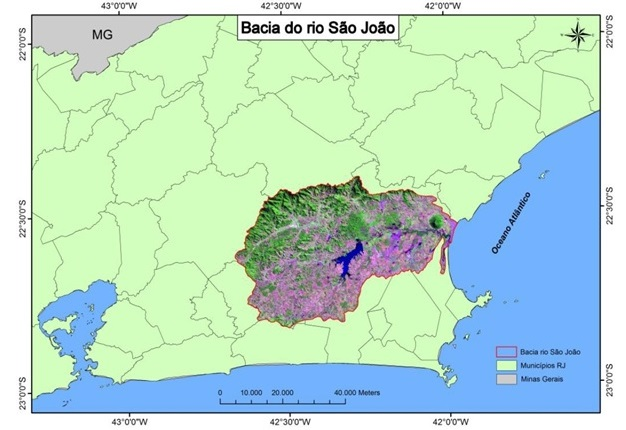
\includegraphics[width=1\textwidth]{C:/Users/eduardo/Documents/Data/Mestrado/BHRSJ.jpg} 
	\caption{Localização da área de estudo.}
	\label{fig:locareaestudo}
	\end{figure}

A partir das obras do DNOS com a retilinização dos canais, problemas sedimentológicos foram gerados devido a diminuição da retenção da água, causando a erosão das margens. Além disso, houveram problemas relacionados ao alagamento de certas localidades e o consequente abandono das mesmas. \\

	\begin{figure}
	\centering
	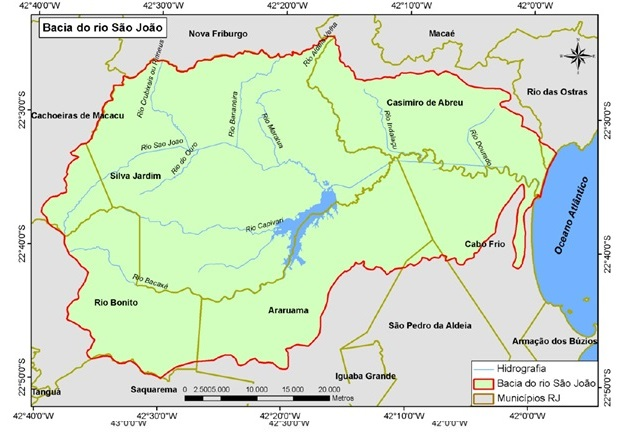
\includegraphics[width=1\textwidth]{C:/Users/eduardo/Documents/Data/Mestrado/BHRSJ_2.jpg} 
	\caption{Municípios inseridos na Bacia do rio São João.}
	\end{figure}

A BHRSJ possui ainda um contexto ambiental no qual vem apresentando uma taxa de recuperação florestal devido ao posicionamento das áreas degradadas perto de áreas de cobertura vegetal, o que vem favorecendo tal recuperação como demonstrado por Seabra \& Cruz (2013) \cite{SEABRA_CRUZ}. Tais características favorecem ainda mais a escolha da BHRSJ como uma área para um estudo de caso no trabalho proposto aqui. \\

	
	\part{Revisão Bibliográfica}
	\chapter{Revisão bibliográfica e pesquisa operacional}
Antes de tudo, o trabalho se dedica a entender através de uma busca bibliográfica a antiga relação entre Geógrafos e a análise de dados através de métodos computacionais, principalmente em relação ao uso de SGBD sejam eles geográficos ou não. 

A relação da Geografia com a utilização de técnicas computacionais é antiga e possui uma forte ligação com os estudos sobre espistemológica da Geografia principalmente no Brasil, onde houve um distanciamento acadêmico dos métodos quantitativos apesar da utilização de ferramentas geotecnológicas por grande parte dos acadêmicos. A busca pelo entendimento da relação entre Geógrafos e a utilização de técnicas tradicionais ligadas a métodos quantitativos esbarra em uma vasta bibliografia onde tenta-se explicar as tomadas de decisão pela Geografia brasileira ao longo de sua história principalmente ao discutir sua dicotomia. 

Grande parte do esforço em coletar bibliografias para a realização deste trabalho envolveu uma pesquisa sobre o estado da arte do desenvolvimento e das aplicações envolvendo banco de dados geográficos mesmo em áreas do conhecimento não necessariamente relacionadas a Geografia. O motivo disso se deu pela dificuldade de se estabelecer um limiar analítico do que poderia ou não ser aplicado como técnica a estudos geográficos. Sendo assim, este trabalho contou com uma vasta pesquisa bibliográfica em áreas como Geografia, Computação, Ecologia, Filosofia, entre outros. 

Com isso, muitos estudos, principalmente envolvendo a primeira grande quebra de paradigma epistemológico na Geografia e a aplicação dos primeiros modelos, assim como os primeiros modelos computacionais se mostram importantes. Se torna essencial entender as relações entre os estudos derivados da Filosofia Analítica, a \textit{Nova Geografia} e o início do desenvolvimento da Geocomputação. É a partir desse entendimento epistemológico que a metodologia para este trabalho passa a fazer mais sentido. A pesquisa bibliográfica foi necessária para se entender cada um desses processos históricos é essencial para tentarmos entender o pensamento do especialista que necessita transformar a paisagem em um modelo representativo de forma sistêmica e integrada através de técnicas computacionais. 

Além disso, tal bibliografia busca entender como as relações epistemológicas e paradigmáticas entre o fazer geográfico no Brasil influenciam o uso de determinadas técnicas. Tenta mostrar também como a influência do desenvolvimento do pensamento geossistêmico e muitas vezes crítico dialético influenciou e ainda influencia não somente a aplicação das técnicas, mas seu desenvolvimento atual. 

A bibliografia existente na área de banco de dados é igualmente vasta e possui uma boa gama de trabalhos já consolidados na academia. A pesquisa bibliográfica se baseou desde trabalhos clássicos como o de Codd (1970)\cite{CODD}, passando por clássicos modernos como Elmasri \& Navathe (2006)\cite{ELMASRI_NAVATHE} até estudos novos na área de banco de dados NoSQL como o de Redmond \& Wilson (2012)\cite{REDMOND_WILSON} ou de Sadalage \& Fowler (2012)\cite{SADALAGE_FOWLER}. Além disso, há um grande interesse de entender através desse trabalho as tecnologias de armazenamento e análise de dados de natureza geográfica, portanto, muitos trabalhos na área de banco de dados geográficos como Casanova et al. (2005)\cite{CASANOVA_etal05} foram explorados. Além disso, trabalhos mais antigos e clássicos voltados para o armazenamento de dados espaciais como o Spatial databases: A tour (SHEKHAR \& CHAWLA, 2003)\cite{SHEKHAR_CHAWLA}, e o Spatial Databases with application to GIS (RIGAUX et al., 2002)\cite{RIGAUX_etal02}, ajudaram a entendermos melhor questões técnicas específicas relacionadas ao processamento de geometrias dentro do banco.

Já a utilização de trabalhos como o de Frank (2003)\cite{FRANK} e Sowa (2000)\cite{SOWA} mostraram a relevância de se entender o conceito de ontologia dentro dos estudos de banco de dados geográficos e na área da geocomputação como um todo. Estudos como estes reforçam ainda mais a ideia de que o entendimento do mundo real, de fato, influencia ao transformar parte dele em informação computacional modelada. Já outros trabalhos como Urbano \& Cagnacci (2014)\cite{URBANO_CAGNACCI} e Agouris \& Croitoru (2005)\cite{AGOURIS} fogem um pouco do objetivo desta pesquisa por trabalharem com banco de dados espaço-temporais. No entanto, apesar de fugir ao objetivo principal, entender o desenvolvimento e a aplicação de banco de dados geográficos que armazenam elementos espaciais que variam ao longo do tempo possibilitam um melhor entendimento não só das possibilidades de aplicação, mas também da interpretação do especialista ao transformar realidade em modelo. É explorado também bibliografias que demonstram novas aplicações na área geotecnológica utilizando sistemas NoSQL, banco de dados baseado em arrays, técnicas de modelagem de dados georreferenciados e problemáticas envolvendo grandes infraestruturas de dados espaciais como no trabalho de Oosterom \& Zlatanova (2008)\cite{OOSTEROM_ZLATANOVA}. 

\chapter{Evolução e história computacional na Geografia}
A interação da população com seu local de origem se expandiu. A percepção do seu espaço de vivência aumenta cada vez mais não só para o qual se está de fato presente, mas para também os que somente virtualmente são possíveis de se alcançar. Local, espaço, território e paisagem são conceitos exaustivamente estudados e cuidadosamente distinguidos pela Geografia. No entanto, a disseminação de tecnologias baseadas em informações e dados espaciais confunde o usuário em perceber com quais delimitações conceituais se está trabalhando exatamente. Esta dificuldade deriva do crescente aumento no acesso a informação e, principalmente, das possibilidades de interação que são permitidas a este usuário(QUATTROCCHI \& GOODCHILD, 1997)\cite{QUATTROCCHI_GOODCHILD}. A consolidação da GeoWeb trouxe ao mundo esta possibilidade. A possibilidade de se localizar espacialmente a qualquer momento, de visualizar informações, de acesso a dados georreferenciados através de um computador pessoal, \textit{smartphone} ou \textit{tablet} e, principalmente, de interagir recebendo informações, assim como gerá-las. 

O recente aumento de interatividade homem-máquina surgiu com o desenvolvimento e consolidação de sistemas de informação geográfica na web, servidores de mapas e dos bancos de dados geográficos. O mapa “clicável” do início da década passada passa então a não ser tão mais interessante como era anteriormente. Gerar a própria informação através dos dados georreferenciados distribuídos publicamente passa a ter um maior apelo para o usuário final. Já a distribuição de dados e informações espaciais passa também, além do setor público e privado, a fazer sentido para o usuário comum, que através de aplicativos geográficos na web começam a interagir com grandes bases de dado e a gerar informação útil, interativa e de qualidade. 

A qualidade desses dados, pesar de questionável, tem sido cada vez mais relacionada a uma produção individual e descentralizada, bastante diferente do que se via a décadas atrás, onde praticamente qualquer geração de dados geográficos dependia de instituições ligadas ao estado ou de grandes corporações. Tal característica foi uma das principais críticas realizada pela Geografia brasileira na década de 1970 aos métodos quantitativos que estavam sendo aplicados (ARMOND, 2013)\cite{ARMOND}. Os dados eram poucos e não existia uma preocupação por parte das instituições de garantir a transparência necessária. Com projetos como o OpenStreetMaps (ARSANJANI et al., 2015)\cite{ARSANJANI_etal15}, muitos dos dados utilizados no processamento de dados georreferenciados atual começa a ser gerados por muitos indivíduos, o que gera ruído, mas possuem a possibilidade de serem estatisticamente tratados de acordo com seu tamanho. Houve uma evolução computacional indiscutível, mas houve também uma evolução na ação de como o Geógrafo coleta os dados e consequentemente os analisa. As novas geotecnologias dão também a possibilidade de aproximar ainda mais sujeito do objeto. 

Esta evolução computacional possui uma relação histórica com os dados de natureza geográfica e com a Geografia em si. Sendo assim, este capítulo tem a função de explicar como a evolução das técnicas computacionais possibilitaram o desenvolvimento de muitos dos sistemas utilizados pela Geografia até os dias de hoje. 

Até duas décadas atrás, a única forma de se gerenciar informações geográficas em formato digital era agrupando todas as informações em um único computador pessoal. O compartilhamento de dados geográficos era realizado necessariamente no mundo real, sendo impossível sua implementação através das já existentes redes virtuais. Tal limitação se devia ao grande tamanho dos arquivos e a quantidade restrita de informação na qual os equipamentos de rede podiam suportar. Além disso, a difusão de dados geográficos digitais só pode de fato,  iniciar sua consolidação com a difusão dos computadores pessoais, dos primeiros sistemas operacionais com interface gráfica, da internet e da web. 

O aumento significativo da capacidade de processamento dos computadores domésticos, assim como o de compartilhamento de dados, armazenamento e visualização dos mesmos, possibilitou que mesmo não especialistas pudessem ter acesso a informações georreferenciadas  através da web. Os Sistemas de Informação Geográfica (SIG), que antes processavam dados apenas na camada offline, agora poderiam ser implementados em arquiteturas cliente – servidor, mudando a forma com que o usuário visualiza e interage com a informação geográfica. 

No entanto, a maior parte dessa evolução e da quebra de alguns paradigmas tecnológicos só foi acontecer a partir da segunda metade da década de 1990, quando a internet abriu suas portas para o mundo extra acadêmico. O estabelecimento e padronização de protocolos de comunicação sob uma rede de telefonia já existente facilitou ainda mais tal difusão. Na mesma época, o hardware dos computadores pessoais passaram a se tornar cada vez mais padronizados e compatíveis com sistemas operacionais que visavam o mercado doméstico. Além disso, o estabelecimento de interfaces gráficas (GUI - \textit{Graphical User Interface}) foi essencial para que a \textit{World Wide Web} transformasse toda aquela arquitetura de redes acadêmicas e militares distribuídas em um ambiente popular de troca de dados e informações (TANENBAUM, 2002)\cite{TANENBAUM_02}.

Esse ambiente interativo e distribuído sofre então uma nova evolução no início dos anos 2000, quando linguagens de script como o ECMAScript (JavaScript), o PHP (PHP: \textit{Hypertext Preprocessor}, originalmente \textit{Personal Home Page}) e muitas outras passam a viabilizar páginas web interativas e esteticamente melhores. É bom lembrarmos que este aumento de interatividade e implementação de novas tecnologias só foram possíveis de acordo com a inovação da própria internet, que neste momento passou a adotar conexões DSL (\textit{Digital Subscriber Line}) e ADSL (\textit{Asymmetric Digital Subscriber Line}) como padrão do mercado. 

Este tipo de conexão teve um papel importante em todo este processo, pois aumentou de forma significativa a quantidade de dados que poderia ser transmitida entre os computadores interconectados em rede. Além disso, por ser um tipo de conexão que poderia ser implementada sob as linhas telefônicas convencionais, não era necessário a troca de toda a estrutura de comunicação, facilitando sua difusão no mercado. O tipo de conexão DSL normalmente funciona transmitindo dados digitais através de fibra óptica ou de cabos de cobre, variando a velocidade de download entre 256kbit/s até 100Mbit/s. Esta variação de velocidade tem suas limitações quando implementada em fios de cobre já que obedece a equação proposta por Shanon (1948)\cite{SHANNON}, onde calcula-se a quantidade máxima de dados possível de ser transmitido por um determinado tipo de material até que este material aqueça o suficiente e inicie um processo de perda de dados (pacotes). O cabo de cobre tem como limite o que seria aproximadamente 8Mbit/s (TANENBAUM, 2011)\cite{TANENBAUM_11}. Além disso, a mesma linha telefônica pode ser dividida em 3 camadas: Camada de Voz (0 – 4Khz), \textit{Upload} (4Khz – 50Khz) e \textit{Download} (50Khz – 1Mhz). Sendo assim, mesmo utilizando fios de cobre datados da década de 1950, ainda hoje é possível encontrar grande parte da estrutura telefônica do país utilizando este mesmo modelo de transmissão de dados digitais. 

A adoção de modelos de transmissão de dados como a ADSL teve papel fundamental da distribuição de conteúdo geográfico na web. Com uma conexão “banda larga”, o usuário poderia receber conteúdo com um grau de interação muito maior do que os possíveis de serem gerados utilizando-se somente HTML (\textit{Hyper Text Markup Language}). Além disso, houve finalmente a liberação do acesso a internet por tempo ilimitado, já que a mesma não poderia mais ser taxada através de “pulsos”. Este tipo de liberdade impulsionou ainda mais a utilização da rede e de seus serviços. 

Os avanços de hardware foram acompanhados pelos avanços na aplicação de desenvolvimento de linguagens de programação que tirassem proveito destas vantagens. Com o aumento de capacidade de troca de dados com conexões de maior banda e do processamento interno dos computadores, linguagens como JavaScript e PHP se tornaram extremamente populares em toda a web. A escolha pela utilização destas linguagens é explicada pelo seu funcionamento interno. O JavaScript é considerado uma linguagem “\textit{Client-Side}”, ou seja, utiliza o processamento do computador do usuário através da interpretação do código-fonte utilizando o navegador (\textit{browser}) para a geração de conteúdo. Já o PHP é considerado uma linguagem “\textit{Server-Side}”, interpretando o código-fonte no servidor onde encontram-se os dados para só assim transmitir ao usuário. O uso massivo de linguagens como o JavaScript alavanvou verbas visando gastos em pesquisa a fim de otimizar cada vez mais as \textit{engines} de interpretação de códigos gerados pelo \textit{browser} do usuário. Essas \textit{engines} de interpretação saíram de modelos simples no início dos anos 2000 para modelos extremamente complexos nos dias atuais. Diferentemente da compilação, a interpretação de códigos-fonte de linguagens de \textit{script} como o JavaScript e o PHP é feita em tempo real (JIT compiler ou \textit{Just in Time compiler}). Sendo assim, o tempo de processamento gasto pelo hardware para otimizar o código que está sendo interpretado de acordo com a arquitetura do processador é menor que quando o mesmo código é compilado (como no caso de linguagens como C, C++, etc), já que a interpretação é feita em “tempo real” para o usuário. No entanto, caso estes mesmos \textit{scripts} fossem compilados, a interatividade e o conteúdo dinâmico oferecido pelos serviços web não seriam funcionais. Enquanto programas compilados ganham em desempenho e estabilidade, programas interpretados ganham na possibilidade de serem extremamente dinâmicos e orientados a serviços. Não existe, portanto, uma linguagem perfeita que contemple todas as vantagens de forma integrada. 

Como consequência dos avanços de hardware, software e transmissão de dados, houveram avanços significativos na visualização no conteúdo gerado e processado. Assim como na visualização científica, a geovisualização teve grandes avanços derivados da evolução computacional. 

Com novas possibilidades de visualização de conteúdo geográfico, a cartografia digital não precisou alterar os conceitos cartográficos básicos já existentes, mas pode adicionar funcionalidades. Além disso, é certo dizer que houve um significativo aumento na complexidade na aquisição e estruturação desses dados, mostrando a necessidade de uma readequação das normas e padrões para que esta informação atendesse a geometria e a topologia esperada. A partir da metade da década de 1990, a cartografia digital passou a incorporar metodologias de representação não lineares, assim como um aumento significativo de interação com o usuário. O conceito de visualização geográfica (ou geovisualização) foi apresentado neste mesmo contexto por autores como Dent (1999)\cite{DENT}, Peterson (1995)\cite{PETERSON}, MacEachren (1995)\cite{MacEACHREN} e Sluter (2001)\cite{SLUTER} (MENEZES \& FERNANDES, 2013)\cite{MENEZES_FERNANDES}. 

Os avanços no campo da visualização geográfica foram inicialmente consequências diretas da evolução da computação gráfica e do desenvolvimento de SIGs. O desenvolvimento de interfaces gráficas, programação orientada a objeto, engines gráficas,, a difusão de GPUs (Graphics Processing Unit) entre computadores pessoais e o surgimento de APIs (\textit{Application Programming Interface}) de desenvolvimento como o OpenGL (\textit{Open Graphics Library}) (SHREINER et. al., 2013)\cite{SHREINER_etal13} em 1992 e o DirectX (LUNA, 2008)\cite{LUNA} em 1995 foram grandes marcos nessa evolução. 

Sendo assim, podemos observar que a aplicação desses recursos são bem recentes. A Geografia saiu da aplicação de modelos computacionais simplificados para a visualização e interação de dados geográficos complexos a pouco mais de uma década. Muitos cientistas passaram a adotar nomes como GeoWeb (LONGLEY et al., 2011)\cite{LONGLEY_etal13}  e Geo Computação (ABRAHART et al., 2014)\cite{ABRAHART} nos últimos anos devido as enormes mudanças ocorridas na relação em que a Geografia vem estabelecendo com a Tecnologia da Informação. Openshaw (2014)\cite{OPENSHAW} observa ainda que o termo “Geo Computação” deve ser considerado um termo novo, já que somente nos últimos anos foi de fato percebido uma quebra de paradigma na forma com que passamos a utilizar estes recursos computacionais. O mesmo autor nos lembra que à duas décadas atrás, a aplicação computacional na Geografia era muitas vezes considerada suficientemente boa de acordo com as aplicações da época. Sendo assim, o autor questiona se o aumento de poder computacional significativo observado e suas novas tecnologias podem ser consideradas, de fato, inovadoras. Ao final, o autor chega a uma conclusão positiva. Openshaw (2014)\cite{OPENSHAW} observa que mesmo em aplicações em que o resultado final era concretizado (apesar do tempo de processamento ser muitas vezes enorme), os modelos e métodos computacionais aplicados à duas décadas atrás eram muitas vezes versões simplificadas, para que houvesse ao menos algum nível de processamento. Sendo assim, a evolução no tempo de processamento da informação geográfica está quase sempre ligada, também, a uma evolução metodológica e dos modelos que são aplicados. 

\chapter{Uma Geografia de quarto paradigma?}
A partir desda mesma ideia, trabalhos como o realizado por Hey et al. (2009)\cite{HEY_etal09} intitulado “\textit{The Fourth Paradigm: Data-Intensive Scientific Discovery}”, mostram as ideias de Jim Gray em defender a existência de uma mudança de paradigma em curso no fazer científico da ciência atual, entendendo que tais mudança derivam diretamente de um aumento nunca antes visto na geração e acumulação de dados e informações por todo o mundo. No entanto, as técnicas e ferramentas de análise que temos, assim como a própria evolução computacional, ainda não dão conta de suprir as necessidades de todas as análises que desejamos. Dentro desse contexto, a utilização de ferramentas e técnicas de armazenamento surgiram como uma peça central no ato de fazer ciência em muitos laboratórios, como defendido por Szalay \& Blakeley (2009)\cite{SZALEY_BLAKELEY}. 

As novas tecnologias de armazenamento tentam solucionar a dificuldade na transferência de grandes quantidades de dados através de protocolos e ferramentas tradicionais como o FTP e o GREP. O desenvolvimento de tais tecnologias não conseguiu acompanhar o aumento no tamanho e na quantidade de dados acumulados. Sendo assim, o gerenciamento de grandes quantidades de dados tornou-se essencialmente distribuído e paralelizado. A transferência da pergunta (\textit{query}) para o servidor é muito mais fácil e rápida de ser executada do que a transferência dos arquivos para o analista.

Muitas ferramentas e técnicas de análise estatística (geralmente espaciais) para o tratamento de dados distribuídos e paralelos foram incorporados ao vocabulário cientifico atual. Empresas do setor privado com capacidade e interesse de investir em novas tecnologias passaram assim a desenvolver ferramentas de análise próprias, o que ainda ocorre nos setores dependentes de uma verba mais restrita (como instituições públicas de pesquisa). Os menos privilegiados, em sua grande parte, ainda dependem de ferramentas de análise mais restritas e de uso mais geral. No entanto, nos últimos anos podemos perceber um crescimento considerável no uso de tecnologias \textit{open source} mesmo no mundo corporativo. 

Jim Gray ainda nos alerta sobre a natureza incerta na escolha de certas técnicas e ferramentas por essa mesma comunidade. Muitos produtos, sendo eles comerciais, ou não, são desenvolvidos, mas poucos deles se tornam populares. Apenas de não ser possível afirmar com certeza o que define o sucesso de uma determinada ferramenta, o autor lembra que o importante é desenvolver e implementar muitas delas. Eventualmente, alguma será escolhida pela comunidade. 

Outra grande característica da ciência de quarto paradigma é a criação de grandes centros de armazenamento de dados abertos. A implementação de grandes bases de dados abertas surge não só como um facilitador na distribuição de dados para a própria comunidade científica, mas como um esforço para a popularização do conhecimento acadêmico ao grande público. Diferentemente da distribuição atual, a nova forma de publicação de conhecimento cientifico propõe que tal divulgação deva ter além de sua parte textual esperada, os arquivos necessários para uma possível replicação do experimento. Muitas dessas ferramentas, sejam elas ligadas ou não a Geografia, são recentes e acabam necessitando de um conhecimento ainda maior do usuário sobre a técnica, o que nem sempre acontece. Mesmo desconsiderando questões epistemológicas e particularidades da Geografia brasileira, pode se dizer que muitas das técnicas ainda não são maduras o suficiente para serem implementadas popularmente, o que restringe, e muito, seu uso.

\chapter{História do pensamento geográfico, modelos e geoinformática.}
A reprodução do mundo real em ambientes computacionais é um sonho para nós humanos a muitas décadas. A representação da realidade em toda sua complexidade certamente pode ser encarada como um dos grandes desafios da ciência da computação. A importância deste desafio vem da possibilidade de aplicação de algoritmos de simulação da realidade em ambientes controlados para entender melhor possíveis cenários, evitando assim a necessidade de realizar testes com efeitos nocivos ao ambiente. As possibilidades de uma possível representação computacional fiel da realidade são inimagináveis. No entanto, apesar da incrível evolução computacional das últimas décadas, ainda precisamos recorrer a modelos.

O conceito de modelo por si só implica a necessidade da abstração. A transformação da realidade para um ambiente computacional deve seguir critérios de generalização de acordo com a informação que seu desenvolvedor deseja gerar. Modelos computacionais foram criados e aplicados desde o início da história da computação e vem sendo largamente utilizados nos mais diversos campos do conhecimento humano. A Geografia é um desses campos. 

\section{Influências analíticas para um novo paradigma do pensamento científico e geográfico}
Grande parte dos modelos computacionais utilizados na Geografia passaram a ser desenvolvidos e implementados a partir da década de 1960 com a popularização da Geografia Quantitativa, também chamada de Nova Geografia (\textit{New Geography}). Os pesquisadores que seguiam tal linha de pensamento tinham como princípio a busca pela aplicação do método hipotético-dedutivo nos estudos geográficos. Por uma forte influência do desenvolvimento de estudos ligados a filosofia analítica (WOLF, 2015)\cite{WOLF} e dos novos métodos computacionais, a ideia adotada pelos pesquisadores era de que a aplicação do método hipotético-dedutivo seria de fato, a melhor forma de capturar esta realidade (mesmo que de forma aproximada) já que utilizava os princípios lógicos e da matemática (POPPER, 1975)\cite{POPPER} (CÂMARA et. al, 2004)\cite{CAMARA_etal04}.

A Geografia foi então fortemente influenciada pelas ideias propostas por Wittgenstein (1961)\cite{WITTGENSTEIN} e a tese do paralelismo lógico-físico, onde a estrutura da linguagem utilizada corresponde a realidade. Segundo Bertrand Russell, o ato de entender a realidade como dizemos ser, assim como entender suas relações lógicas e suas verdades, depende da forma lógica com que falamos sobre ela. Sendo assim, segundo a filosofia analítica, somente a linguagem matemática poderia ser legítima como um instrumento de conhecimento, já que ela possui a limitação da própria lógica em sua representação. Como consequência da popularização do método analítico, o paradigma matemático passa então a ser adotado por muitas disciplinas científicas como metodologia em busca de rigor, coerência e objetividade, tendo o "princípio da verificabilidade" como principal fundamento. Uma consequência deste fato foi a possibilidade de universalizar muitos procedimentos científicos, unificando os métodos em uma única linguagem lógica (GOMES, 2011)\cite{GOMES}.

Gomes (2011)\cite{GOMES} nota ainda que a influência do pensamento analítico, principalmente na Geografia física, possibilitou que a noção de objeto fosse substituída por uma noção de sistemas. Essa troca de conceitos influenciou como consequência a aplicação da teoria geral dos sistemas em outras disciplinas como a Geografia. A noção de sistemas trouxe a ideia de hierarquia e conexão entre os elementos, facilitando o desenvolvimento de modelos ambientais principalmente a partir da década de 1950. Trabalhos como o de Shaefer (1953)\cite{SCHAEFER} surgem então para defender a ideia de uma possível transição entre uma Geografia clássica e moderna. A Geografia Idiográfica de Hartshorne (1939)\cite{HARTSHORNE} passa a não ser mais considerada ciência por muitos. Mais tarde, trabalhos como o livro \textit{Explanation in Geography} de Harvey (1969)\cite{HARVEY} surgem para solidificar ainda mais as contribuições da ciência analítica e do pensamento baseado na aplicação de paradigmas de generalização e refutação.

Se utilizando da mesma fundamentação, a Física surge como uma espécie de modelo para a constituição de uma ciência dita moderna, ideia posteriormente criticada por Latour (1994)\cite{LATOUR}. Este modelo contribui então para o estabelecimento de uma certa necessidade no estabelecimento de leis gerais que operam na manifestação de fenômenos. A formulação de leis como a "Lei de Tobler" por Waldo Tobler surgiram dentro desse mesmo contexto. Para Tobler (1970)\cite{TOBLER}, "tudo está relacionado entre sí. Mas coisas (objetos) próximos se relacionam mais do que objetos distantes."

Como posteriormente discutido por Santos (2006)\cite{SANTOS_06}, a valorização das ciências naturais consequentemente provocou a adoção de uma tendência reducionista não somente na Geografia, como em todas as ciências sociais. Pressionados, muitos passaram a adotar métodos quantitativos que vemos como consequência deste processo até hoje, como o preenchimento de formulários em pesquisas.

Nesta mesma época, muitos cursos relacionados a departamentos ligados às ciências sociais fecharam as portas pela influência dos ideais neopositivistas Na Geografia, departamentos importantes como o departamento de Geografia da Universidade de Harvard, Chicago e UC Davis foram obrigados a se dissolver por não serem "científicos o suficiente", e isso somente nos EUA. 

Seguindo esta transformação paradigmática denominada por Ian Burton (1963)\cite{BURTON} de "revolução quantitativa e teorética da geografia", o fazer geográfico deveria basear seus estudos na utilização de métodos quantitativos através do acúmulo de dados e principalmente na ideia de descrição organizacional dos fenômenos no espaço. A utilização de conceitos como o de região perderam força dando lugar a uma saturação do uso do conceito de espaço. A Geografia passa então a consolidar epistemologicamente seus subcampos (hidrologia, pedologia, climatologia, biogeografia, etc) e consequentemente segmentando o conhecimento geográfico. Novamente, é importante notar que tal processo não foi exclusivo da Geografia, sendo na verdade uma característica em que toda a ciência sofreu durante esse mesmo período.

Nesta mesma época, a utilização de computadores como uma ferramenta de análise espacial começava a se tornar popular, influenciando inclusive o desenvolvimento dos primeiros SIG na década de 1970. O surgimento desses primeiros SIG foram importantes para que a aplicação de modelos tomassem outra dimensão, sendo aplicados cada vez mais dentro de ambientes computacionais. No entanto, o desenvolvimento de métodos analíticos esbarrava não só em sua limitação linguística e lógica, mas também em limitações técnicas. O desenvolvimento da computação, por melhor que fosse, não poderia solucionar (ainda) muitos dos problemas de processamento, armazenamento e visualização dos dados da época. Portanto, a aplicação de modelos era certamente limitada a apenas alguns estudos. Tal dificuldade teve influencia direta ao questionamento tanto das técnicas utilizadas como também na qualidade que os dados processados apresentavam não somente antes como também depois do processamento.

Pouco a pouco, a partir de críticas principalmente realizadas pelo estabelecimento de um pensamento crítico-dialético na Geografia brasileira marcado pela reunião da AGB de 1978, e também por análises como as realizadas por Christofoletti (1985)\cite{CHRISTOFOLETTI}, avaliaram que muitos dos trabalhos publicados durante este período mostravam uma clara má utilização dos métodos quantitativos. Chegou-se a conclusão de que a utilização de técnicas estatísticas não poderiam garantir uma melhor interpretação dos fenômenos espaciais. Para a compreensão dos fenômenos geográficos seria necessário possuir além de técnicas quantitativas, bases conceituais teóricas para a interpretação dos resultados. Sendo assim, o uso de técnicas quantitativas deveria ser um meio, e não o fim (ARMOND, 2013)\cite{ARMOND}.

\section{A alternativa geossistêmica}
A partir dessa insatisfação da comunidade geográfica pela falta de integração entre seus subcampos e pelo aumento da dicotomia entre o dito "físico" e o "humano", surgem trabalhos como os realizados por Bertrand (1968)\cite{BERTRAND} e o de Sotchava (1977)\cite{SOTCHAVA}, marcando assim a introdução da teoria geossistêmica no Brasil. A abordagem geossistêmica já considerava influências da "ação antrópica", o que já ocorria na geomorfologia e na climatologia à época (ARMOND, 2013)\cite{ARMOND}.

Com o estabelecimento da teoria geossistêmica, outros conceitos fundamentais na Geografia como o de paisagem que anteriormente tinham sido deixados de lado acabaram sendo repensados e reformulados para entender o objeto de estudo de uma forma integrada. Nesta mesma época, o conceito de paisagem era utilizado de forma mais restritiva, sendo usado somente para categorizar tipos específicos de paisagens como "paisagem vegetal" ou "paisagem cultural". Segundo Bertrand (1968)\cite{BERTRAND}, o conceito de paisagem deveria apresentar uma perspectiva de análise mais geográfica do que ecológica, como acontecia com o conceito de "meio", bastante utilizando na mesma época.

Apesar das diferenças conceituais entre os trabalhos de Bertrand e Sotchava, Monteiro (2001)\cite{MONTEIRO_01} diagramou um modelo de aplicação da ideia de geossistemas baseando-se em quatro etapas: análise de variáveis naturais e antrópicas, integração entre os elementos de acordo com o problema diagnosticado e finalmente as etapas de síntese e aplicação. Neste momento, ainda existia a ideia de uma clara separação entre o antrópico e o social, relação que viria a sofrer mudanças com o tempo. Mendonça (2005)\cite{MENDONCA} critica esta separação por entender que, por essência, desde sua gênese, não deveria existir uma oposição entre homem e natureza. Os movimentos sociais ligados as reivindicações do movimento negro, das mulheres e dos ecologistas estudados por Porto-Gonçalves (2006)\cite{PORTO_GONCALVES} que surgiram na década de 60 e 70, principalmente a partir de Estocolmo em 1972 e com a famosa "\textit{blue marble}" (Figura \ref{fig:bluemarble}), fizeram os estudiosos a evidenciar a disputa de concepções entre natureza e sociedade (ARMOND, 2013)\cite{ARMOND}. 

	\begin{figure}
		\centering
		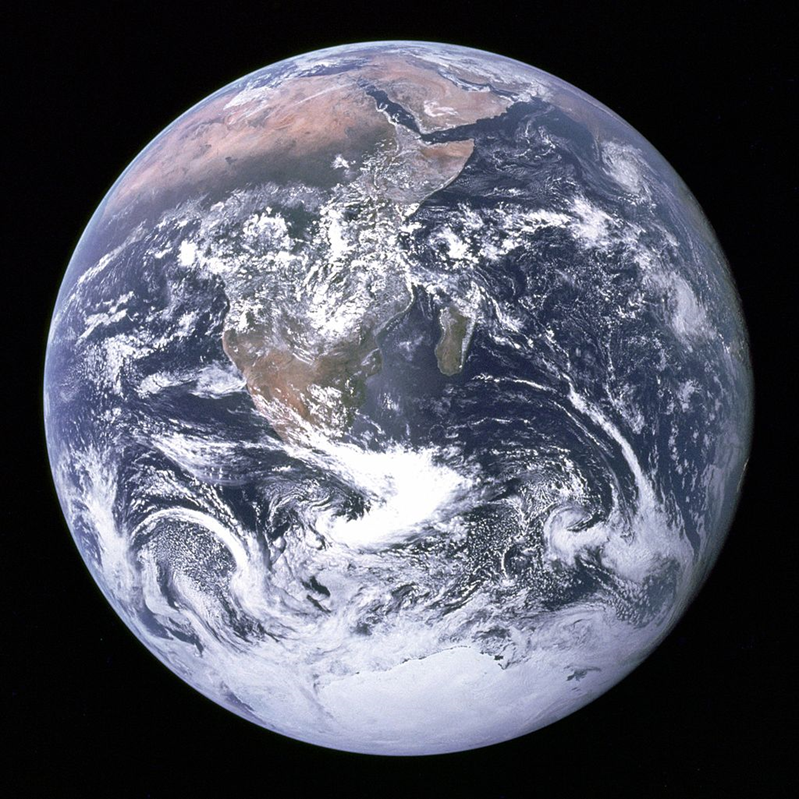
\includegraphics[width=0.9\linewidth]{data/blue_marble}
		\caption{A "The Blue Marble" foi a primeira imagem da terra vista dessa distância, sendo uma importante ferramenta para os primeiros questionamentos ambientais. A imagem foi capturada pela tripulação da Apollo 17 em 1972.}
		\label{fig:bluemarble}
	\end{figure}

A incorporação da teoria geral dos sistemas nas ciências naturais e na Geografia passou então a ganhar força, onde muitos pesquisadores passaram a incorporar métodos disponíveis em ciências correlatas para aplicar em seus estudos (CHRISTOFOLETTI, 1985)\cite{CHRISTOFOLETTI}. Sendo assim, muitos modelos passaram a ser aplicados e desenvolvidos a partir de teorias a estudos geográficos, assim como validados através de dados de campo e utilizando métodos estatísticos Chorley \& Haggett (1967\cite{CHORLEY_HAGGETT} apud CÂMARA\cite{CAMARA_etal04} et. al., 2004).

Trabalhos pioneiros como o de Batty (1976\cite{BATTY76}; 1984\cite{BATTY84}) na área urbana da Geografia mostraram que o desenvolvimento de modelos geográficos computacionais continuaram a se desenvolver mesmo antes das grandes inovações geocomputacionais da década de 1990, onde os primeiros SIGs com interface gráfica surgiram. Mesmo antes das inovações gráficas, muitos modelos passaram a ser aplicados com suporte computacional, onde integravam cada vez mais tecnologias inovadoras como o uso da Inteligência Artificial, Redes Neurais, Bancos de Dados, Matemática Fractal, Modelos Baseados em Agentes, Algoritmos Genéticos, Autômatos Celulares e Lógica Nebulosa (Fuzzy Logic) (BURROUGH \& FRANK, 1996\cite{BURROUGH_FRANK}; OPENSHAW \& OPENSHAW, 1997\cite{OPENSHAW_OPENSHAW}) (CÂMARA et. al., 2004)\cite{CAMARA_etal04}.

As inovações tecnológicas pós década de 2000 passaram então a influenciar novas aplicações além de um retorno na popularidade dos modelos na Geografia, principalmente com o desenvolvimento de softwares de modelagem como o SLEUTH (CLARKE et al., 1997\cite{CLARKE_elal97}; CLARKE \& GAYDOS, 1998\cite{CLARKE_GAYDOS}; SILVA \& CLARKE, 2002\cite{SILVA_KEITH}), softwares de modelagem nacionais como o desenvolvido pelo Centro de Sensoriamento Remoto da Universidade Federal de Minas Gerais (CSR-UFMG) denominado "DINAMICA EGO" (SOARES-FILHO et al., 2009)\cite{SOARES_FILHO_etal09}, trabalhos utilizando autômatos celulares em cidades do interior de São Paulo como o realizado por Almeida (2003)\cite{ALMEIDA} e Almeida et. al. (2003)\cite{ALMEIDA_etal03},  além de publicações importantes como o trabalho de Benenson \& Torrens (2004)\cite{BENENSON_TORRENS} onde o termo Geosimulação é cunhado, assim como a continuação do mesmo em Marceau \& Benenson (2011)\cite{MARCEAU_BENENSON}.

No entanto, devido principalmente ao período de ditadura militar, muitos questionamentos foram feitos em relação a quantificação do saber geográfico e na aplicação de modelos. Questionava-se por exemplo não somente o método em sí, mas a qualidade e legalidade dos dados obtidos para os estudos, já que grande parte desses mesmos dados proviam de instituições públicas que ofereciam apenas dados extremamente restritos e limitados. Existia uma clara deficiência em relação a confiabilidade dos dados disponíveis. Monteiro (2006)\cite{MONTEIRO_06} lembra que o ano de 1984 marcou de forma clara o início da dicotomia entre Geografia "Humana" e "Física" no Brasil com a criação do Simpósio Brasileiro de Geografia Física Aplicada e do Seminário de Geografia Aplicada, onde muitos dos geógrafos ditos "físicos" possuíam uma evidente carência de reflexão política e epistemológica, gerando inclusive um certo mal-estar em relação a comunidade geográfica com um todo.

Esta fragmentação, em parte, se deu também pela evolução técnica e instrumental desigual ocorrida entre as áreas do conhecimento geográfico como descrita por Nunes et al. (2010):	
	
	\begin{quote}
		"Enquanto a Geologia, Meteorologia e as engenharias, por exemplo, conheceram uma significativa evolução tecnológica, resultado do progresso científico, a Geomorfologia, a Climatologia e mesmo a Pedologia, ramos do conhecimento que se relacionam de forma estreita com aquelas ciências, não foram suficientemente rápidas para absorver estes novos conhecimentos e incorporar o instrumental técnico.
		Essa compartimentação já foi mais intensa, mas ainda é perceptível na abordagem ambiental da Geografia Física, que expõe a paisagem natural de modo explicativo, sem relacionar as atividades humanas nos seus estudos."
	\end{quote}

A partir da década de 80, começa então a surgir referências teóricas que buscavam o estabelecimento do fazer científico e consequentemente geográfico mais conjuntivo derivado das reflexões sobre a compartimentação dos saberes. Trabalhos como o realizado por Santos (2006)\cite{SANTOS_06} e Latour (1994)\cite{LATOUR}, assim como os questionamentos sobre a ideia de certeza apresentada por Prigogine (1996)\cite{PRIGOGINE}, são exemplos de críticas a uma ciência dita moderna que não leva em consideração questionamentos e abordagens transdisciplinares ao gerar um esfacelamento do conhecimento.

Reflexões sobre uma Geografia mais conjuntiva e voltada em entender a paisagem através de uma perspectiva ambiental e sistêmica foram desenvolvidas por Suertegaray e Nunes (2001)\cite{SUERTEGARAY_NUNES} e Suertegaray (2004)\cite{SUERTEGARAY}, onde se estudou o processo em que a Geografia brasileira passou a entender a questão ambiental não somente pelo seu lado "físico", mas também por sua dimensão socioeconômica. Segundo a autora, não faz mais sentido pensar em Geografia sem que se pense de uma forma integrada internamente e também externamente Suertegaray (2004\cite{SUERTEGARAY} apud ARMOND, 2013\cite{ARMOND}). 

Segundo a mesma autora, a sociedade contemporânea estaria cada vez mais preocupada em saber como funcionam os sistemas ambientais do que em tentar responder o por que de funcionarem de tal maneira. Daí a importância de se pensar a questão ambiental a partir de suas bases filosóficas e políticas. 

Trabalhos como os citados servem para ajudar a pensar os SIG atuais assim como novas geotecnologias visando a transformação da Geocomputação em uma disciplina menos estática. Autores como Câmara et. al. (2004) defendem a ideia de que os SIG da próxima geração devem incorporar ferramentas de modelagem para entender a evolução dos fenômenos analisado-os através de representações funcionais. Ou seja, a incorporação de modelos preditivos, análises espaço-temporais e multi-escalares devem ser cada vez mais presentes nos estudos geográficos, já que assim relações dinâmicas podem ter a chance de serem estudadas com ajuda do computador.

 
\section{Por uma Geografia mais conjuntiva}

A Geografia atual vem tentando encontrar um equilíbrio entre o desenvolvimento técnico e científico, buscando compreender o estudo da paisagem utilizando não somente métodos quantitativos como qualitativos. Este tipo de integração vem, nos últimos anos, sendo alvo de autores pertencentes a diversas áreas do conhecimento geográfico.

A busca pelo fazer geográfico integrado vem mostrando discussões teóricas e técnicas como o desenvolvimento de um SIG crítico proposto por Acselrad et al. (2008)\cite{ACSELRAD} e as novas formas de integração entre dados quantitativos e o qualitativos como proposto por DeLyser \& Sui (2011\cite{DELYSER_SUI_11}, 2012\cite{DELYSER_SUI_12}, 2013\cite{DELYSER_SUI_13}).

Segundo a trilogia de artigos publicados por Dydia DeLyser, professora de Geografia Humana na Louisiana State University e Daniel Sui, professor de Geotecnologias da Ohio State University, a Geografia atual passa por uma forte reformulação conceitual e epistemológica principalmente devido as influências do constante desenvolvimento geotecnológico e principalmente pelo estabelecimento de um novo paradigma do fazer científico como proposto por Hey et al. (2009)\cite{HEY_etal09}.

O surgimento do que os autores chamam de "\textit{digital humanities}" como uma aliança entre \textit{nerds} e poetas (COHEN, 2010)\cite{COHEN}, representa um momento de mudança metodológico na pesquisa acadêmica como um esforço de transdisciplinaridade. A noção de "ciência má" e "ciência boa" como criticada por Morin (2005)\cite{MORIN} passa a dar lugar a busca por um fazer científico crítico e integrado. Sendo assim, a partir da utilização da informática, existe a possibilidade nunca antes vista de se coletar uma grande quantidade de dados diretamente dos usuários e também de analisar tais bases em busca de informações classificadas de acordo com seu contexto. Na verdade, a noção de contexto na computação vem sendo uma das grandes revoluções dentro das aplicações computacionais dentro das ciências humanas.

Visões políticas como o esforço pela divulgação de dados de forma transparente, principalmente por instituições governamentais vem influenciando a acumulação de dados sociais e ambientais, assim como no esforço pela criação de grandes infraestruturas de dados espaciais, com o objetivo de sustentar de forma organizada toda essa abertura. Além disso, muitos sistemas modernos passaram a registrar dados geográficos dos usuários de muitas das ferramentas mais utilizadas com o intuito de beneficiar principalmente a venda de novos serviços. Apesar de sua natureza questionável, muitos dos dados podem ser coletados de forma legal e utilizados para muitos outros estudos além do marketing.  

DeLyser e Sui apresentam uma grande gama de estudos que estão sendo realizados dentro dos departamentos de Geografia nos EUA que além de possuírem uma característica conjuntiva, apresentam como característica a aplicação de técnicas computacionais mesmo em estudos tipicamente qualitativos. Outra característica apresentada pelos autores é que grande parte dos dados coletados e armazenados nos grandes bancos de dado possuem uma natureza temporal. Os dados, além de espaciais, possuem quase sempre, a possibilidade de serem analisados no tempo, característica encontrada também em estudos geossistêmicos modernos. O aumento significativo de material de análise, assim como a evolução do hardware e do software possibilitou que geógrafos passassem a entender a leitura da paisagem digitalmente, assim como o de qualquer outra conceito geográfico fundamental através do tempo. Busca-se com isso entender os processos.

Autores como Sheller \& Urry (2006)\cite{SHELLER_URRY} defendem inclusive o termo "revolução móvel", por entenderem que a popularização de tecnologias móveis como o \textit{smartphone} servem como uma mudança de paradigma na forma em como buscamos, acumulamos e analisamos dados espacias. Aplicações como o \textit{Google "n-gram" database} podem servir para que geógrafos estudem quantitativamente uma quantidade enorme de dados buscando entender contextos culturais que antes seriam impossíveis de serem estudados.

Estudos utilizando bases de dados derivados de sites de busca, sensores, registros telefônicos ou em postagens em mídias sociais como o Facebook e o Twitter (JÜRGENS \& JUNGHERR, 2016)\cite{JURGENS_JUNGHERR} são exemplos da possibilidade de integração de ferramentas computacionais modernas com os estudos dos fenômenos geográficos. Muitos desses estudos tem como perspectiva um caráter espaço/temporal assim como histórico/geográfico, integrando múltiplos modos de análise por parte do geógrafo. Trabalhos como os realizados por Borgman (2009), Sieber et al. (2011)\cite{SIEBER_etal11}, Bodenhamer et al. (2010)\cite{BODENHAMER_etal10}, Daniels et al. (2011)\cite{DANIELS_etal11}, Dear et al. (2011)\cite{DEAR_etal11} e Berry (2012)\cite{BERRY}, são exemplos de como as ciências humanas no geral pode se beneficiar da era do \textit{big data}, buscando mais sinergia entre as metodologias aplicadas aos estudos geográficos (DeLyser \& Sui, 2012)\cite{DELYSER_SUI_12}.

\section{Problemas na representação do conhecimento geográfico}

Durante muito tempo, pesquisadores na área da Geografia estudaram a relação entre os processos de ocupação do espaço com os fluxos e interações decorrentes de suas ações. Autores como Milton Santos, David Harvey e Manuel Castells desenvolveram trabalhos significativos servindo como base para mostrar que grandes esforços ainda devem ser feitos pela Ciência da Geoinformação a ponto de realizar tais análises dentro de um ambiente puramente computacional. Tais autores se empenharam em desenvolver estudos voltados a compreensão do espaço não só como um ambiente estático, mas como um espaço de interações contínuas, múltiplas e multi-escalares. A representação desse mesmo espaço através de sistemas computacionais estáticos passa então, pouco a pouco, a fazer menos sentido. 

No entanto, estudos que trabalham com a abordagem de conceitos geográficos mais abstratos ainda não possuem forma possível de implementação nos sistemas computacionais atuais. A modelagem e implementação de componentes sócio-econômicos, assim como a aplicação de algoritmos que trabalhem com fluxos de elementos multi-escalares se tornou um dos maiores desafios da computação atual. A arquitetura de hardware, assim como a implementação de softwares, ainda é feita baseando-se na aplicação de lógica booleana e derivando equações matemáticas formais. Logo, a análise de dados para a geração de informação computacional complexa o suficiente para atender os novos conceitos utilizados pela Geografia moderna, só poderão ser realizadas com o uso de um sistema computacional igualmente complexo. Autores como Penrose (1989)\cite{PENROSE} discutem tais problemas buscando entender o funcionamento lógico, físico e filosófico da computação eletrônica atual. No entanto, para alcançar tamanha complexidade, os sistemas computacionais deveriam ser estimulados a evoluírem a ponto de possuírem pensamentos próprios iguais ou até mesmo mais complexos que o de um ser humano. Em \textit{"The Emperor's New Mind: Concerning Computers, Minds, and the Laws of Physics"} Penrose (1989)\cite{PENROSE} aborda já no primeiro capítulo questões que tenta responder com o decorrer do livro: Poderiam os computadores pensar? É possível o desenvolvimento de uma inteligência não-natural? Será que um computador poderá possuir inteligência igual ou superior a de um ser humano? Tais questionamentos são a base de estudos na Inteligência Artificial desde a publicação do famoso trabalho de Turing (1950)\cite{TURING}, e vem servindo como parâmetro para uma possível evolução e quebra de paradigma no funcionamento dos sistemas computacionais atuais. Mudanças dessa magnitude possibilitariam aplicações nunca antes vista em nossa sociedade, além de quebras de paradigmas em toda a ciência, incluindo a Geografia.

Segundo autores como Câmara et. al. (2004)\cite{CAMARA_etal04}, o estado atual das geotecnologias pode satisfazer por completo somente modelos geográficos quantitativos. É importante notar, no entanto, que a discussão proposta por Câmara onde SIG atuais seriam classificados de acordo com os paradigmas da Geografia Quantitativa, não necessariamente implica que trabalhos desenvolvidos pela Ciência da Geoinformação sejam quantitativos. Um estudo geoinformacional por sí só não tem como premissa se basear apenas na aplicação de componentes e análises derivadas de aplicações computacionais. A análise geográfica deve ser maior que sua implementação eletrônica. No entanto, os SIG do futuro como representado por Câmara no mesmo trabalho, possuem características que poderiam analisar e representar o conhecimento geográfico de uma forma nunca antes vista. Tais mudanças possibilitariam, por exemplo, a implementação de SIG críticos como o proposto por Sheppard (2008)\cite{SHEPPARD}.

Sendo assim, a Geografia estruturada em relações espaciais complexas baseadas nos conceitos de forma, função, estrutura e processo, deve encontrar um modo de implementa-las utilizando-se dos meios computacionais tradicionais. No entanto, os sistemas informacionais digitais atuais encontram problemas na aplicação de conceitos mais abstratos pois ainda baseiam-se necessariamente na materialização das noções de espaço. Ou seja, a visualização do espaço em um ambiente computacional necessita de uma conexão a um aspecto físico/geométrico para ser representado. Seria então possível realizar uma transição de conceitos abstratos como a ideia de fluxos trabalhada por Santos (1978)\cite{SANTOS} e Castells (1999)\cite{CASTELLS} ou como a de "sistemas de objetos e de ações" por Santos (1996)\cite{SANTOS_96} para um ambiente computacional? Haveriam limitações?

Em seus estudos sobre a representação do conhecimento em ambientes computacionais, Sowa (2000)\cite{SOWA} apresenta a ideia de que para transportar conceitos e elementos do mundo real para um ambiente computacional é estritamente necessário que o especialista entenda primeiramente as interações lógicas, ontológicas e de implementação do modelo:

	\begin{quote}
		"Sem a lógica, a representação do conhecimento é vaga e sem critérios para determinação de quais declarações são redundantes ou contraditórias. Sem a ontologia, os termos e símbolos são mal definidos e confusos. E sem os modelos computacionais, a lógica e a ontologia não podem ser implementadas em softwares. A representação do conhecimento é a aplicação da lógica e da ontologia visando a construção de modelos computacionais para alguma área do conhecimento." (SOWA, 2000)\cite{SOWA}.
	\end{quote}

Entendendo melhor o pensamento de Sowa, podemos concluir que o desenvolvimento de modelos computacionais, de dados, assim como de SIG envolve o uso de diversos conceitos que interagem constantemente entre sí. O sucesso na implementação de qualquer sistema ou modelo depende do planejamento de cada um desses conceitos apresentados pelo autor. Ignorar um dos conceitos não é uma opção. Sendo assim, podemos finalmente entender que a aplicação de conceitos mais abstratos como o "sistema de objetos e ações" trabalhado por Santos (1996)\cite{SANTOS_96}  em sistemas computacionais, apesar de possuir forte base teórica conceitual na Geografia, possui uma falta de maturidade lógica e ontológica ao interagir com as técnicas atuais de modelagem de dados. Autores como Câmara nos mostra ainda que tal transição esbarraria em limitações não somente na criação de modelos baseados em "objetos e ações", mas também em suas representações e interações.

Mesmo entendendo a evolução das ferramentas, métodos e seus conceitos envolvidos, a modelagem do espaço continua sendo uma tarefa extremamente complexa. Esta dificuldade existe pois o processo de abstração e discretização de elementos geográficos no espaço ainda é realizada de forma subjetiva. O especialista deve respeitar regras lógicas, utilizar uma ontologia, entender as técnicas computacionais envolvidas neste processo, se questionar sobre a escala adotada e ainda a necessidade ou não de uma possível padronização dos dados. Por final, o especialista deve ficar atento a questões de funcionalidade e representatividade do seu modelo.

Modelos geográficos, assim como SIG acabam servindo como próteses intelectuais, alargando nossas capacidades cognitivas. Sendo assim, é importante notar que o desenvolvimento de modelos e sistemas, assim como as informações apresentadas pelos menos, podem se tornar soluções hegemônicas. Uma solução geográfica dessa natureza apresenta um forte vínculo entre o conhecimento que os edifica e a solução por eles edificada (CASTIGLIONE, 2009)\cite{CASTIGLIONE}. Portanto, cabe ao especialista o dever de estar atento ao processo de modelagem de dados e/ou do sistema, pois o modelo criado se transformará na legitimação da "realidade" modela. Para isso, precisamos antes entender cada etapa do processo do desenvolvimento.

\section{A elaboração de modelos de dados geográficos.}

Por ser apenas uma generalização, o modelo deve abstrair e se concentrar em apenas alguns tipos de informação, possuindo uma ou mais funcionalidades. Sendo assim, cabe ao especialista entender perfeitamente qual será o uso do modelo, utilizando somente as ontologias que lhe irão servir.
Para este serviço, algumas métodos foram criadas para organizar melhor o pensamento do especialista. O paradigma dos quatro universos (Figura \ref{fig:paradigmaquatrouniversos}) proposto inicialmente por Gomes \& Velho (1995)\cite{GOMES_VELHO} e posteriormente adaptado para a geoinformação por Câmara (1995)\cite{CAMARA} surgiu com este intuito.

	\begin{figure} [h]
		\centering
		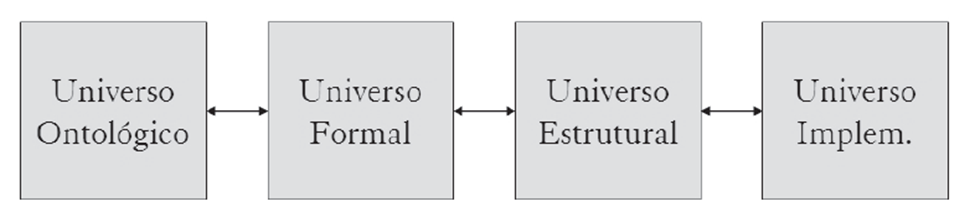
\includegraphics[width=1\linewidth]{data/paradigma_quatro_universos}
		\caption{Paradigma dos quatro universos.\cite{CAMARA_b}}
		\label{fig:paradigmaquatrouniversos}
	\end{figure} 

	

	\textbf{Universo Ontológico:} \\

	O primeiro passo se baseia na tarefa de descrição da realidade nas entidades necessárias que precisamos para entender o que estamos estudando.  A criação do universo ontológico representa a transformação de elementos como tipos de solo, área urbana, geomorfologia para conceitos que serão representados pelo computador. \\
	
	\textbf{Universo formal:} \\
		
	Já o universo formal, trata de incluir modelos lógicos e matemáticos que generalizam os conceitos propostos pelo universo ontológico. O universo formal tenta responder a pergunta: Quais são as abstrações formais necessárias para representar os conceitos de nosso universo ontológico? É dentro desde universo que o especialista tem a tarefa de escolher qual o melhor modelo de dados para abstrair tais ontologias. Modelos como o entidade-relacional (CHEN, 1976)\cite{CHEN}, UML (RUMBAUGH el al., 2004)\cite{RUMBAUGH_etal04}, OMT (RUMBAUGH el al., 1991)\cite{RUMBAUGH_etal91} e OMT-G (DAVIS et al., 2002)\cite{DAVIS_etal02} são exemplos de modelos que podemos utilizar neste processo de construção. \\
	
	\textbf{Universo estrutural:} \\
	
	O terceiro universo é o universo estrutural, que é responsável por transformar os modelos formais em estruturadas de dados geométricas e alfanuméricas. \\
	
	\textbf{Universo de implementação:} \\
	
	 Por último, temos o universo de implementação. Esta etapa é a responsável por transformar toda a parte conceitual em aplicação. É onde fazemos as escolhas das arquiteturas que utilizaremos.
	 
	 \section{Modelagem de dados e estudos de favorabilidade}
	 
	 Dentre as muitas aplicações que a modelagem de dados geográficos pode servir, a aplicação e desenvolvimento de modelos para a área ambiental vem crescendo significativamente.  Uma das possíveis aplicações são nos estudos voltados a estimativa de favorabilidade ambiental de certas áreas.
	 
	 Seabra (2012)\cite{SEABRA} trabalha com o termo favorabilidade entendendo que o mesmo é utilizado na literatura principalmente em trabalhos que visam indicar áreas com maior possibilidade de ocorrência de recursos ou fenômenos naturais. Além disso, destaca que o termo também é utilizado em trabalhos que visam classificar de forma hierárquica áreas onde a ação humana poderia se dar de forma mais eficiente, visando a diminuição dos custos econômicos e ambientais, seja para a implementação de industrias, exploração mineral ou até mesmo na escolha de áreas de preservação.
	 
	 A favorabilidade é normalmente calculada na forma de índice através da análise de critérios múltiplos. Tais estudos utilizam diversos tipos de variáveis que tentam englobar a maior quantidade possível de dados, no entanto, estudos sobre favorabilidade baseiam-se apenas em um conjunto restrito de fatores que consideramos relevantes, sendo impossível a consideração de todos (SEABRA, 2012)\cite{SEABRA}. O processo de transformação das informações adquiridas no mundo real para a criação de um estudo de favorabilidade seguem as mesmas regras de criação dos modelos de dados, daí o porque das suas restrições semânticas, de implementação e de análise. Apesar disso, são muitos os tipos de estudos sobre favorabilidade que podemos realizar. Incluindo os sobre favorabilidade à recuperação florestal.
	 
	 Seabra (2012)\cite{SEABRA} entende favorabilidade à recuperação florestal como a capacidade do geossistema em restabelecer as condições estruturais e de funcionamento necessárias para que ocorra a recuperação de áreas degradas. Sendo assim, é essencial que se entenda o funcionamento do sistema através de uma análise multi-escalar e hierárquica. Além disso, o autor aponta a importância da consideração de fatores abióticos, bióticos e socioeconômicos para a melhor compreensão dos processos e interações, como é trabalhado por Crk et al. (2009)\cite{CRK_etal09}, Rudel el al. (2000)\cite{RUDEL_etal00} e Chazdon (2003)\cite{CHAZDON}. Estes estudos apontam a importância do uso de variáveis para além dos fatores bióticos afim de demonstrar melhores resultados. A incorporação dessas novas variáveis torna a análise final ainda mais complexa e adiciona uma quantidade de dados considerável, demonstrando que estudos dessa natureza podem se beneficiar não só das técnicas de modelagem como de integração dos dados em um SGBD espacial.
	 
	 \section{Modelos de dados geográficos}
	 
	 Na área de banco de dados, autores como Elmasri \& Navathe (2006)\cite{ELMASRI_NAVATHE} definem modelo como o conjunto de conceitos que podem ser usados para descrever a estrutura e as operações em um banco de dados (BORGES et. al, 2005)\cite{BORGES_etal05}.
	           
	   Modelos de dados semânticos e orientados a objetos como ER (CHEN, 1976)\cite{CHEN}, OMT (RUMBAUGH et al., 1991)\cite{RUMBAUGH_etal91}, IFO (ABITEBOUL \& HULL, 1987)\cite{ABITEBOUL}, UML (RATIONAL SOFTWARE CORPORATION, 1997)\cite{UML}, entre outros, são largamente utilizados não só em aplicações mais gerais como também em aplicações geográficas. No entanto, modelos como os citados não possuem a melhor forma de lidar com dados georreferenciados. Com a popularização na utilização de sistemas operacionais com interfaces gráficas e o desenvolvimento de SIG mais elaborados na década de 1990, SGBD passaram a incorporar extensões espaciais influenciando consequentemente a criação de extensões para modelos de dados convencionais, suprindo algumas necessidades no trabalho de abstração e generalização do mundo geográfico real para o ambiente computacional. Diferentemente dos modelos convencionais, os espaciais apresentam relações de conceitos e entidades, assim como também os tipos de inter-relacionamentos e entidades representáveis necessárias (BORGES et. al., 2005)\cite{BORGES_etal05}.       
	   
	   Modelos como o GeoOOA (KÖSTERS et al., 1997)\cite{KOSTERS_etal97}, MODUL-R (BÉDARD et al., 1996)\cite{BEDARD_etal96}, GMOD (OLIVEIRA et al., 1997)\cite{OLIVEIRA_etal97}, IFO para aplicações geográficas (WORBOYS et al., 1990)\cite{WORBOYS_etal90}, GISER (SHEKHAR et al., 1997)\cite{SHEKHAR_etal97}, OMT-G (BORGES et al., 2001)\cite{BORGES_elat01}, GeoFrame (LISBOA FILHO, 1997)\cite{LISBOA_FILHO} e MADS (PARENT et al., 1999)\cite{PARENT_etal99} surgiram para prover as soluções de abstração do espaço seguindo regras de integridade espacial e se tornando úteis de acordo com o objetivo do especialista ao implementá-los aos SGBD. Borges et. al. (2002\cite{BORGES_elat02} apud CASANOVA et al., 2005\cite{CASANOVA_etal05}).
	   
	   \section{O modelo OMT-G}
	   
	   O modelo OMT-G (\textit{Object Modeling Technique for Geographic Applications}) segue as primitivas de diagramação de classes da UML, mas introduzindo outras de natureza geográfica com o objetivo de aumentar a capacidade de representação semântica (BORGES et al., 2001)\cite{BORGES_elat01}. O modelo se baseia em três conceitos principais: classes, relacionamentos e restrições de integridade espaciais. Além disso, o modelo OMT-G propõe o uso de três diferentes diagramas para o processo de desenvolvimento de uma aplicação geográfica: diagrama de classes, diagrama de transformação e diagrama de apresentação (BORGES \& FERREIRA, 2006)\cite{BORGES_etal05}.
	   
	   \subsection{Diagrama de classes}
	   
		Dentre os três tipos de diagramas existentes, o mais utilizado é o diagrama de classes. Este diagrama é usado para descrever a estrutura e o conteúdo do banco de dados geográfico. Sendo assim, ele define e descreve conceitualmente como os dados do banco serão estruturados através de regras. Além disso, este tipo de diagrama possui a capacidade de organizar informações sobre o tipo de representação que cada classe terá. É a partir do diagrama de classes que é possível derivar um conjunto de restrições de integridade espaciais que deve ser considerado no nível de implementação (BORGES \& FERREIRA, 2006).
	
		\subsection{Classes}
		
		Para criar o diagrama de classes é necessário primeiramente a criação de classes. Existem três grandes grupos de dados que pode representar classes no modelo OMT-G (contínuos, discretos e não-espaciais). Estes três grandes grupos possibilitam que uma aplicação modela de acordo com o modelo OMT-G, possua uma visão mais integradora do espaço, além da possibilidade de uma maior interação entre classes convencionais e georreferenciadas (Figura \ref{fig:omtgclasses}).
		
		\begin{figure} [h]
			\centering
			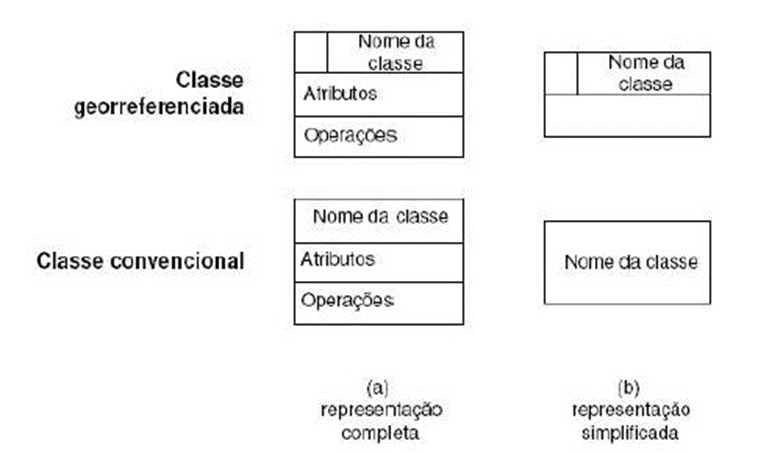
\includegraphics[width=1\linewidth]{data/omtg_classes}
			\caption{Classes georreferenciadas e convencionais no OMT-G.\cite{BORGES_etal05}}
			\label{fig:omtgclasses}
		\end{figure}
	
		Além disso, o modelo OMT-G apresenta uma quantidade fixa de possibilidades de representação geométrica dos dados. Utiliza-se uma simbologia especial em que distingue-se geo-objetos e geo-campos como mostrados na Figura \ref{fig:geocampos} e na Figura \ref{fig:geoobjetos}. O modelo ainda define cinco tipos de classes descendentes de geo-campos: isolinhas, subdivisão planar, tesselação, amostragem e malha triangular (\textit{Triangulated Irregular Network}, TIN), além de duas para classes descendentes de geo-objetos: geo-objeto com geometria e geo-objeto com geometria e topologia (BORGES \& FERREIRA, 2006). 
		
		\begin{figure} [h]
			\centering
			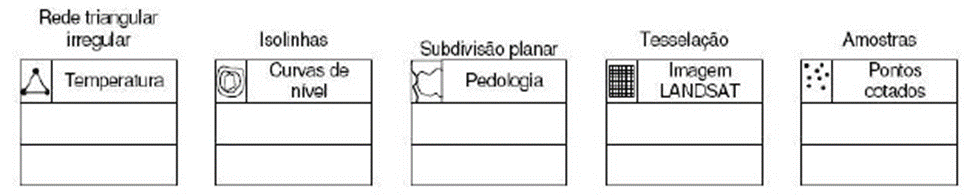
\includegraphics[width=1\linewidth]{data/geocampos}
			\caption{Geo-campos.\cite{BORGES_etal05}}
			\label{fig:geocampos}
		\end{figure}
	
		\begin{figure}[h]
			\centering
			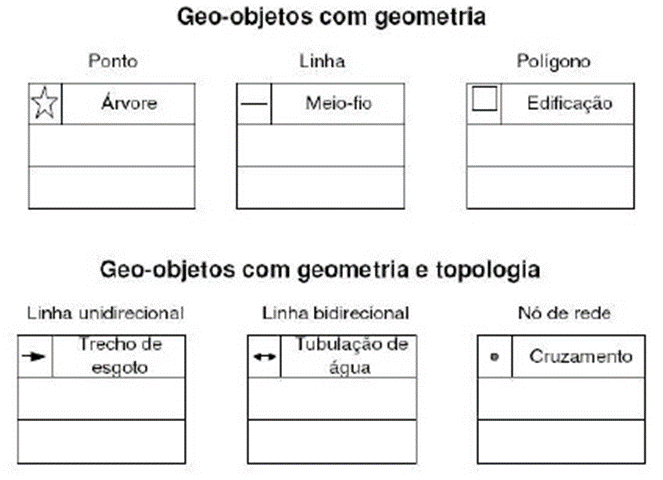
\includegraphics[width=0.9\linewidth]{data/geoobjetos}
			\caption{Geo-objetos.\cite{BORGES_etal05}}
			\label{fig:geoobjetos}
		\end{figure}
		
		\subsection{Relacionamentos}
		
		Em sua lógica de relacionamentos, o modelo OMT-G apresenta três distintos: \textbf{associação simples, relacionamentos topológicos em rede e relacionamentos espaciais}. Borges \& Ferreira (2006) explicam que a associação simples representa os relacionamentos estruturais entre objetos de classes diferentes, convencionais ou georreferenciadas. Já os relacionamentos espaciais representam relações topológicas, métricas, de ordem e \textit{fuzzy}. Por último temos ainda os relacionamentos topológicos, que podem fazer relações derivadas automaticamente a partir da forma geométrica do objeto no momento da entrada dos dados ou da execução de alguma análise espacial (Figura \ref{fig:relacionamentos}).
		
		\begin{figure} [h]
			\centering
			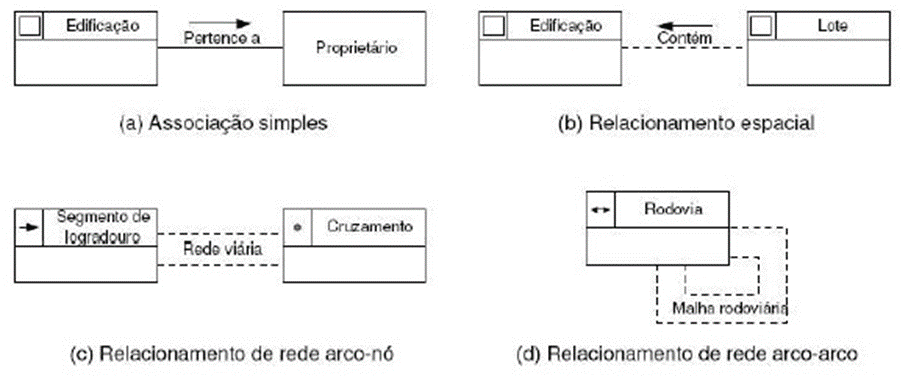
\includegraphics[width=1\linewidth]{data/relacionamentos}
			\caption{Relacionamentos. \cite{BORGES_etal05}}
			\label{fig:relacionamentos}
		\end{figure}
	
		\subsection{Cardinalidade}
		
		Os relacionamentos que podemos construir no modelo são caracterizados por sua cardinalidade. A cardinalidade adotada pelo modelo OMT-G (Figura \ref{fig:cardinalidade}) é a mesma que a utilizada na UML, e representa o número de instância de uma classe que podem estar associadas a instâncias da outra classe (BORGES \& FERREIRA, 2006).
		
		\begin{figure} [h]
			\centering
			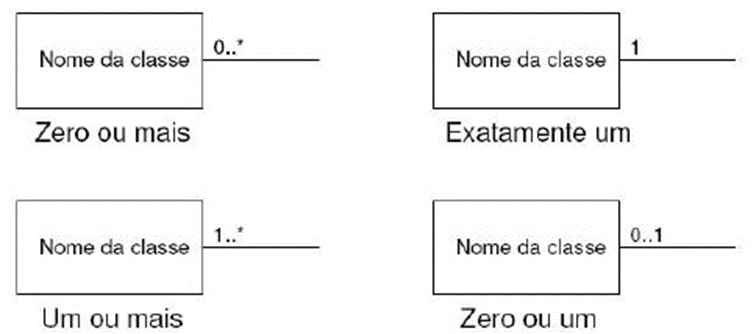
\includegraphics[width=1\linewidth]{data/cardinalidade}
			\caption{Cardinalidade. \cite{BORGES_etal05}}
			\label{fig:cardinalidade}
		\end{figure}
		
		\subsection{Relacionamentos topológicos}
		
		O modelo OMT-G consegue explorar as capacidades semânticas da modela espacial porque entende hierarquicamente as classes e seu relacionamentos de cardinalidade através de relacionamentos topológicos como o estabelecido pela \textit{Open Geospatial Consortium} (OGC) e seu modelo da matriz de 9 interseções (Figura \ref{fig:relactopologicos}).
		
		\begin{figure} [h]
			\centering
			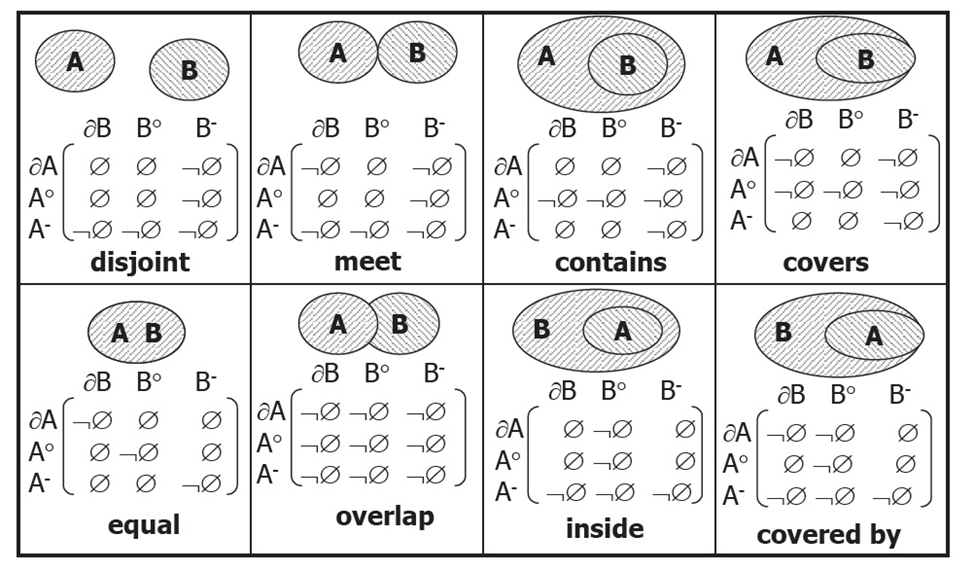
\includegraphics[width=1\linewidth]{data/relac_topologicos}
			\caption{Matriz de 9 interseções para relações entre duas regiões. \cite{EGENHOFER_91}.}
			\label{fig:relactopologicos}
		\end{figure}
		
		\subsection{Outras possibilidades}
		
		O modelo OMT-G permite que o especialista ainda realize a modelagem generalizando ou especializando os dados, de forma que o trabalho de modelar elementos espaciais em diferentes escalas não se torne um problema. Este processo de generalização e especialização ainda pode aplicado tanto a classes georreferenciadas quanto a classes convencionai (Figura \ref{fig:generalizacaoespecializacao}). 
		
		\begin{figure} [h]
			\centering
			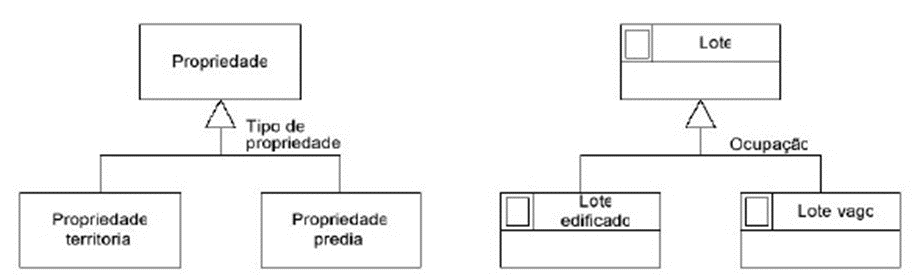
\includegraphics[width=1\linewidth]{data/generalizacao_especializacao}
			\caption{Generalização/Especialização. \cite{BORGES_etal05}}
			\label{fig:generalizacaoespecializacao}
		\end{figure}
		
		Outra característica do modelo OMT-G é possibilitar a agregação de dados. Borges \& Ferreira (2006) definem agregação como a forma especial de associação entre objetos, onde se considera que um deles é formado a partir de outros. É possível ainda realizar agregações espacias. Agregações espaciais são realizadas através de relacionamentos topológicos "todo-parte" (ABRANTES, 1994)\cite{ABRANTES} (KÖSTERS, 1997)\cite{KOSTERS_etal97}. Os autores mostram ainda que a agregação espacial  serve para indicar que a geometria de cada parte deve estar contida na geometria do todo. A superposição entre as geometrias das partes não é permitida, consequentemente a geometria do todo deve ser totalmente coberta pela geometria das partes, configurando uma partição do plano ou subdivisão planar (PREPARATA \& SHAMOS, 1985)\cite{PREPARATA_SHAMOS} Davis (2000\cite{DAVIS} apud BORGES \& FERREIRA, 2006\cite{BORGES_etal05}). A Figura \ref{fig:agregacaoespacial}. apresenta a forma como o modelo OMT-G representa esta notação. 
		
		\begin{figure} [h]
			\centering
			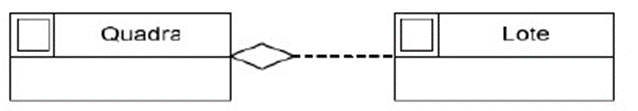
\includegraphics[width=1\linewidth]{data/agregacao_espacial}
			\caption{Agregação espacial ("todo-parte"). \cite{BORGES_etal05}}
			\label{fig:agregacaoespacial}
		\end{figure}
		
		O modelo ainda possibilita a criação de esquemas montando generalizações conceituais utilizando não só a questão da escala, mas variáveis como a forma. A construção de um modelo OMT-G pode ser realizada da mesma forma que qualquer outro tipo de modelagem conceitual de dados. No entanto, é necessário que se tenha as ferramentas computacionais adequadas para a melhor representação e implementação do modelo. Ferramentas como a extensão (Stencil) CASE para o software Microsoft Visio desenvolvido por Karla Borges é um exemplo.  
		
		\section{Arquiteturas e linguagens}
		
		Bancos de dados e sistemas de gerenciamento de banco de dados (SGBD) estão muito mais presentes do que podemos imaginar em nossas vidas; sendo inclusive essenciais em atividades diárias como uma ida ao banco, realizando uma reserva em um hotel ou ao fazer compras online. O uso de banco de dados está presente já a algumas décadas em nossas vidas, no entanto, grande parte de seu uso ainda é feito utilizando-se banco de dados tradicionais, onde a natureza de dado armazenado é normalmente do tipo numérico ou textual (ELMASRI \& NAVATHE, 2006)\cite{ELMASRI_NAVATHE}. No entanto, foi somente com pesquisas realizadas nos últimos anos que estes sistemas passaram a lidar de forma mais integrada com outros tipos de dados. O avanço de tecnologias voltadas ao tratamento de dados geográficos, assim como o constante e considerável aumento na quantidade de dados dessa natureza disponibilizados através da Web fez com que a necessidade por tecnologias de armazenamento de dados espaciais fossem desenvolvidas. Além disso, a integração com Sistemas de Informação Geográfica (SIG) fez com que os bancos de dados relacionais (SGBD-R) também fizessem parte do cotidiano dos usuários de dados georreferenciados.
		
		Muitas das arquiteturas adotadas para o desenvolvimento de SIG variaram conforme a estratégia de armazenamento dos dados. Atualmente, tais sistemas vem evoluindo e buscando uma maior integração com os sistemas de banco de dados geográfico (CASANOVA et al., 2005). Além disso, como consequência de um maior uso, houve um interesse na padronização desses dados, sendo assim, criados padrões como a \textit{Simple Feature} (OGC, 2012a\cite{OGC_12a}; OGC, 2012b\cite{OGC_12b}) e a SQL/MM (MELTON \& EISENBERG, 2001)\cite{MELTON_EISENBERG}. O benefício da padronização no nível de armazenamento foi um ganho na interoperabilidade (QUEIROZ et al., 2013)\cite{QUEIROZ_etal13}.
		
		O constante aumento no volume de dados transferidos e armazenados devida a ampla utilização da internet fez com que em paralelo fossem desenvolvidas tecnologias de banco de dados para lidar com tal tipo de informação de forma mais otimizada. Bancos de dados NoSQL vem se tornando cada vez mais populares, sendo inclusive o tipo de tecnologia de banco de dados com maior crescimento nos últimos anos (ANGLINGER \& GELBMANN, 2015)\cite{ANGLINGER_GELBMANN}. Os sistemas NoSQL vem tendo um papel essencial principalmente no armazenamento e análise de dados derivados exclusivamente da internet, assim como de sistemas de captura de dados digitais contínuos e de dados derivados de dispositivos móveis. Queiroz et al. (2013)\cite{QUEIROZ_etal13} no mostra ainda que a tecnologia NoSQL vem sendo cada vez mais estudada também na área da Geografia e  Geoinformática, como nas pesquisas de (KERR, 2009\cite{KERR}; BAPTISTA et al., 2011\cite{BAPTISTA_etal11}; MALONE, 2010\cite{MALONE}; WANG \& WANG, 2010)\cite{WANG_WANG}.
		
		Sendo assim, a partir de tantas tecnologias disponíveis, este capítulo visa demonstrar de forma introdutória as arquiteturas e linguagens mais utilizadas no campo de banco de dados, assim como uma introdução a tecnologias de armazenamento de dados espaciais, novas tecnologias e, finalmente, apresentar de forma mais aprofundada as que foram utilizadas para a realização deste trabalho.
		
		\subsection{Sistemas de gerência de banco de dados relacionais}
		
		O início das pesquisas e o desenvolvimento de muitas tecnologias ligadas aos sistemas gerenciadores de banco de dados relacionais (SGBD-R) surgiram no laboratório da \textit{International Business Machines} (IBM) em San José, Califórnia. Codd (1970) \cite{CODD} foi quem iniciou tais pesquisas em tal laboratório, desenvolvendo assim o famoso \textit{Modelo Relacional de Dados}.
		
		O modelo proposto por Codd (1970)\cite{CODD} e sua futura implementação teria como uma das características principais o uso de tabelas onde registros como nome da tabela, nome da coluna e numeração das linhas estão quase sempre presentes. O trabalho realizado por Queiroz et al. (2013)\cite{QUEIROZ_etal13} nos mostra que tal modelo se tornou extremamente popular não somente por sua sólida estruturação teórica, mas também pelo desenvolvimento de tecnologias que possibilitaram uma evolução nos bancos de dados. Muitos avanços foram e ainda são realizados no campo de banco de dados baseado no modelo relacional, no entanto, algumas inovações históricas foram fundamentais para a consolidação de tal modelo, como por exemplo:
		
		\begin{enumerate}
			\item O desenvolvimento da tecnologia de indexação principalmente em árvores-b (COMER, 1979) ou por hash (CORMEN et al.,  1990)\cite{CORMEN_etal90}, acelerando o processo de busca e atualização da informação no sistema.
			
			\item A criação do SQL, uma linguagem de alto nível para realizar consultas e manipulação de dados no sistema (MELTON, 2003)\cite{MELTON}.
			
			\item A criação de um modelo de programação baseado no conceito de transações, sendo executadas de forma atômica, satisfazendo as propriedades conhecidas por ACID: atomicidade, consistência, isolamento e durabilidade (ELMASRI \& NAVATHE, 2006)\cite{ELMASRI_NAVATHE}.
			
			\item E finalmente, regras para a replicação de dados, obrigando o banco a obedecer um modelo mestre/escravo, onde consultas de leituras poderiam ser feitas a qualquer nó, mas consultas de escrita somente ao nó mestre.	
		\end{enumerate}
	
		Casanova et al. (2005)\cite{CASANOVA_etal05} nos mostra através de duas tabelas algumas características importantes em sistemas de banco de dados. A Figura \ref{fig:requisitossgbd} nos mostra os requisitos mais importantes para tais sistemas e a Figura \ref{fig:princtecsgbd1} lista as principais tecnologias desenvolvidas para atendê-los.
		
		\begin{figure}
			\centering
			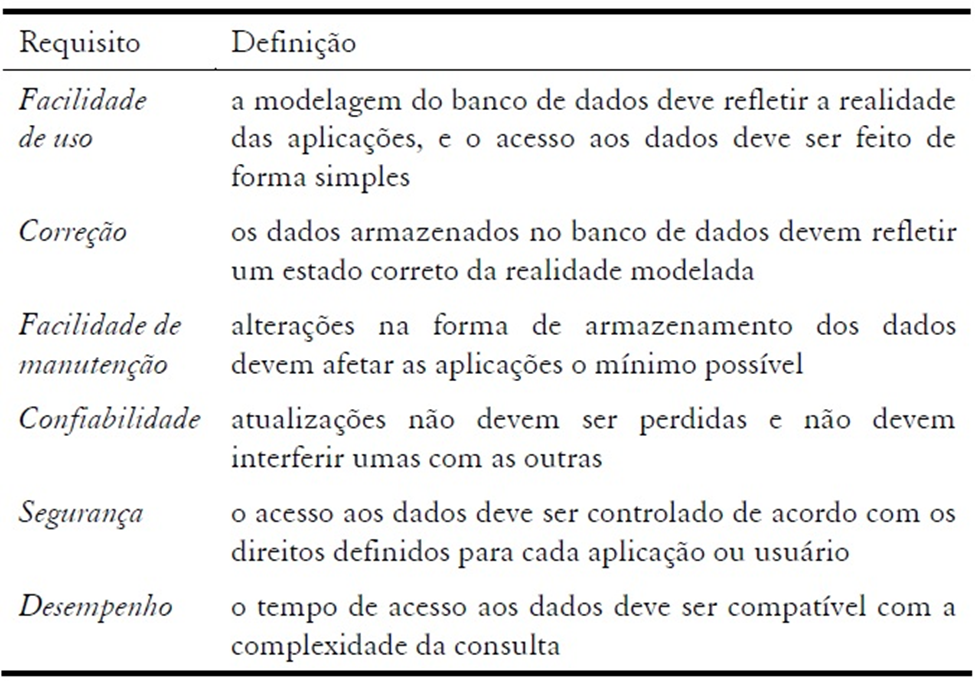
\includegraphics[width=1\linewidth]{data/requisitos_SGBD}
			\caption{Principais requisitos para SGBD. \cite{CASANOVA_etal05}}
			\label{fig:requisitossgbd}
		\end{figure}
		
		
		\begin{figure}
			\centering
			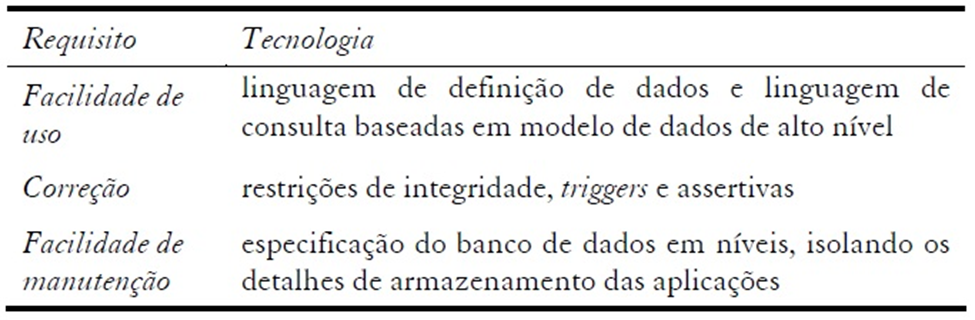
\includegraphics[width=1\linewidth]{data/princ_tec_SGBD_1}
			\caption{Principais tecnologias de um SGBD. \cite{CASANOVA_etal05}}
			\label{fig:princtecsgbd1}
		\end{figure}
		
		\begin{figure}
			\centering
			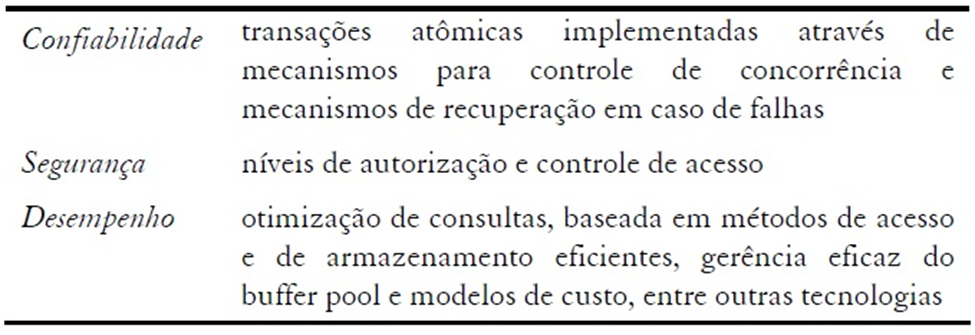
\includegraphics[width=1\linewidth]{data/princ_tec_SGBD_2}
			\caption{Principais tecnologias de um SGBD (2). \cite{CASANOVA_etal05}}
			\label{fig:princtecsgbd2}
		\end{figure}
		
		Os SGBDs mais utilizados no mercado ainda são do tipo SGBD-R, no entanto uma fatia no mercado já utiliza SGBD Objeto-Relacionais (SGBD-OR) e SGBD Orientados-a-Objeto (SGBD-OO). Essa lógica de divisão de mercado existe pelo fato dos SGBD-R serem de fato ainda os melhores ao armazenar dados convencionais. Qualquer tipo de dado que seja um número inteiro, de ponto flutuante, data, caractere ou um campo binário longo (BLOB), será atendido perfeitamente por um sistema convencional. No entanto, qualquer inclusão de dado não convencional em um SGBD-R pode gerar efeitos colaterais gerando uma perna considerável de desempenho no sistema e dificuldades com o processo de codificação Stonebraker (1996\cite{STONEBRAKER} apud CASANOVA et al., 2005\cite{CASANOVA_etal05}).
		
		\subsection{A Structured Query Language (SQL)}
		
		Segundo Elmasri \& Navathe (2006)\cite{ELMASRI_NAVATHE}, a linguagem SQL pode ser considerada um dos principais motivos pelo sucesso dos SGBD-R comerciais. Tal importância é dada porque o SQL se tornou um padrão entre praticamente todos os banco de dados utilizados, sendo assim um facilitador técnico ao migrar aplicações entre diferentes sistemas. Além disso, o autor nos mostra que tal padronização foi importante para que se tornasse possível a utilização de vários SGBG diferentes ao mesmo tempo, já que a linguagem de comunicação para ambos é a mesma.
		
		A linguagem SQL (\textit{Structured Query Language}) foi desenvolvida no início dos anos 1970 pela IBM mas acabou sofrendo algumas alterações ao longo do tempo como mostra a Figura.
		
		\begin{figure}
			\centering
			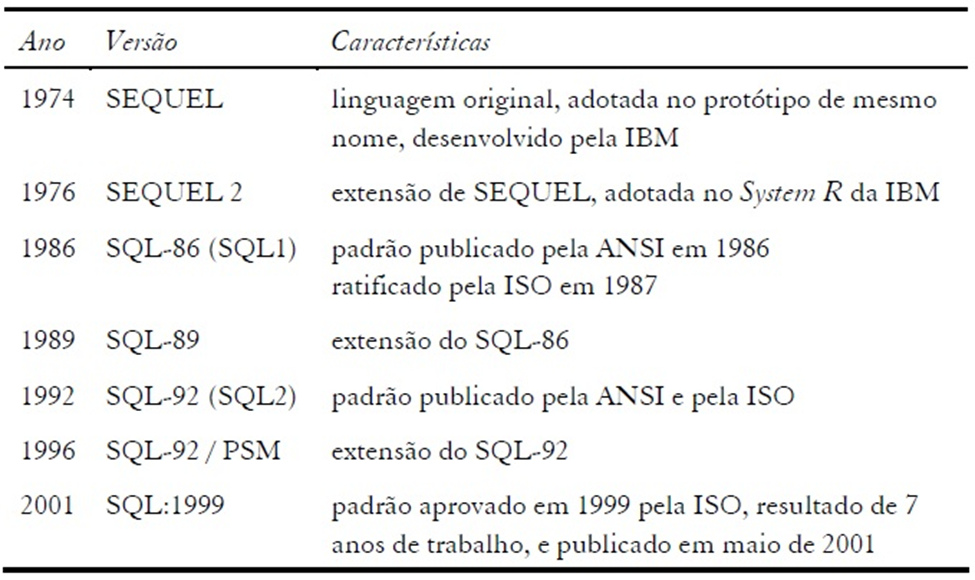
\includegraphics[width=1\linewidth]{data/sql_history}
			\caption{Breve histórico da linguagem SQL. \cite{CASANOVA_etal05}}
			\label{fig:sqlhistory}
		\end{figure}
		
		A linguagem SQL (\textit{Structured Query Language} - Linguagem de Consulta Estruturada) que inicialmente se chamava SEQUEL (\textit{Structured English QUEry Language}), foi inicialmente implementada no sistema relacional System R, também desenvolvido pela IBM. Ela também é considerada uma linguagem abrangente, já que possui funções tanto para definição de dados (DDL - \textit{Data Definition Language}) como para manipulação (DML - \textit{Data Manipulation Language}). Além disso, suas últimas versões possibilitaram que fosse integrada a linguagens de uso geral como C/C++ , Java e COBOL (ELMASRI \& NAVATHE, 2006)\cite{ELMASRI_NAVATHE}.
		
		O SQL é formado por diversos comandos padrões comuns a todos o SGBD que utilizam a linguagem como base. Alguns dos comandos mais utilizados são listados na Figura.
		
		Banco de dados que utilizam o SQL são implementados em grande escala, servindo de base para muitos dos serviços que utilizamos diariamente. Muitos desses serviços possuem um volume de dados armazenados muito grande, mesmo assim, muitas das vezes o código-fonte escrito em SQL para a operação de tais bases não ultrapassam algumas linhas de código como no caso do site Piratebay. O site é famoso por ser considerado o maior \textit{tracker} de arquivos .torrent da internet, possuindo cerca de 8 milhões de arquivos em sua base de dados. No entanto, o código SQL necessário para seu funcionamento não passa de poucas linhas como mostrado à seguir (OPENBAY, 2015)\cite{OPENBAY}:
		
		\newpage
		
		\begin{lstlisting} [float,floatplacement=H]
			DROP TABLE IF EXISTS `torrents`;
			CREATE TABLE IF NOT EXISTS `torrents` (
			`id` int(11) unsigned NOT NULL AUTO_INCREMENT,
			`name` varchar(255) DEFAULT NULL,
			`description` text,
			`category_id` tinyint(4) DEFAULT NULL,
			`size` bigint(20) unsigned DEFAULT NULL,
			`hash` varchar(40) NOT NULL,
			`files_count` int(11) DEFAULT '0',
			`created_at` datetime DEFAULT NULL,
			`torrent_status` smallint(2) DEFAULT '0',
			`visible_status` smallint(2) DEFAULT '0',
			`downloads_count` mediumint(8) unsigned NOT NULL DEFAULT '0' COMMENT                 	   'umax = 16777215',
			`scrape_date` datetime DEFAULT NULL,
			`seeders` mediumint(8) unsigned NOT NULL DEFAULT '0',
			`leechers` mediumint(8) unsigned NOT NULL DEFAULT '0',
			`tags` varchar(500) DEFAULT NULL,
			`updated_at` datetime DEFAULT NULL,
			PRIMARY KEY (`id`),
			UNIQUE KEY `hash` (`hash`),
			KEY `created_at` (`created_at`),
			KEY `size` (`size`),
			KEY `seeders` (`seeders`),
			KEY`category_id_torrent_status_visible_status`     	 (`category_id`,`torrent_status`,`visible_status`)
			);
		\end{lstlisting}
		
		\begin{figure}
			\centering
			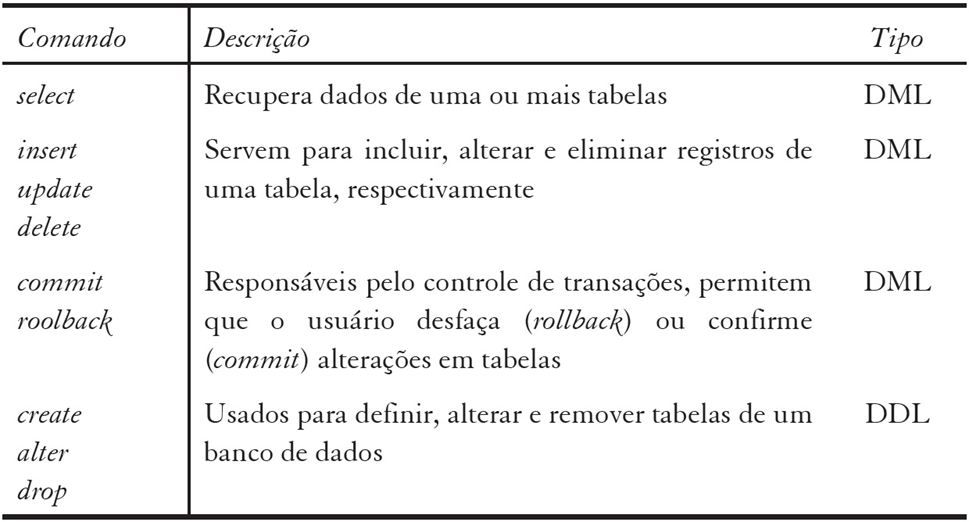
\includegraphics[width=1\linewidth]{data/comandos_sql}
			\caption{Lista de comandos SQL. \cite{CASANOVA_etal05}}
			\label{fig:comandossql}
		\end{figure}
		
		Banco de dados como o do site Piratebay nos permite mostrar que a quantidade de dados armazenados, assim com a importância de um banco de dados, não necessariamente possui relação direta a sua complexidade de implementação. Lembrando que a facilidade na implementação de muitos modelos só é possível devido as vantagens que a linguagem SQL propicia. No entanto, tais arquiteturas e linguagens se tornam restritas quando a aplicação em questão faz uso de atributos espaciais como no caso de banco de dados geográficos e SIG.
		
		Até o SQL-89, consultas espaciais eram um problema já que ainda não eram suportadas pelo padrão. Sendo assim, a partir da década de 1990, estudos como em (EGENHOFER, 1994\cite{EGENHOFER_92}; OGIS, 1995\cite{OGIS}) foram realizados afim de solucionar tais questões e estabelecer um novo padrão. Com o tempo, padrões com o SF-SQL proposto pela OGC através do padrão SQL-92 e a Spatial-SQL desenvolvida por Egenhofer (EGENHOFER, 1994)\cite{EGENHOFER_92} surgiram para tentar soluconar problemas relacionado ao tratamento deste tipo de dado. Muitas extensões espaciais para o SQL foram desenvolvidas principalmente ao final da década de 1980. Extensões como PSQL (ROUSSOPOULOS et al. 1988)\cite{ROUSSOPOULOS_etal88}, Spatial SQL (EGENHOFER 1991\cite{EGENHOFER_91}, 1994\cite{EGENHOFER_92}), GEOQL (OOI \& SACKS-DAVIS 1989\cite{OOI_SAKIS_DAVIS}, OOI et al., 1989\cite{OOI_etal89}, OOI 1990\cite{OOI}), linguagens baseadas em consultas SQL para o KGIS (INGRAM \& PHILLIPS 1987)\cite{INGRAM_PHILLIPS}, e o TIGRIS (HERRING et al. 1988)\cite{HERRING_etal88} foram exemplos desse esforço (EGENHOFER, 1999)\cite{EGENHOFER_etal99}. Mas foi somente com a SQL/MM (MM para MultiMedia) Spatial, associada ao nome SQL:1999 (MELTON, 2003)\cite{MELTON} que passamos a ter uma extensão para tratar texto, dados espaciais e imagem estática ou em movimento (CASANOVA et al., 2005)\cite{CASANOVA_etal05}. Além disso, é importante notar que a manipulação de dados espaciais implica não só na necessidade de uso de linguagens de consulta espaciais especificas, mas também de modelos e arquiteturas que suportem tal tipo de dado.
		
		\subsection{Integração de arquiteturas SIG e SGBD}
		
		A partir da necessidade de integração de dados espaciais e SIGs houve um esforço para que com o tempo, a integração entre SGBD e SIGs fosse consolidada. A integração entre SIGs e SGBD se pode ser feita principalmente de duas formas: através de uma arquitetura dual ou através de uma arquitetura integrada Figura \ref{fig:arquiteturaduaintegrada}.
		
		\begin{figure}
			\centering
			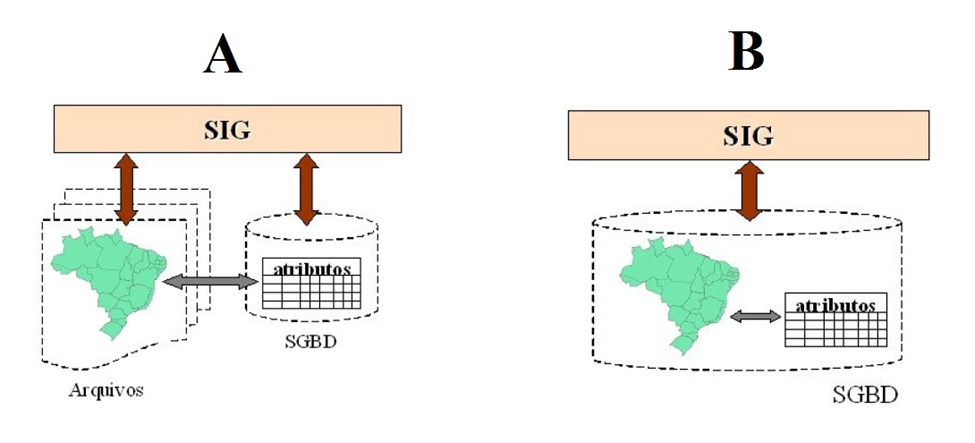
\includegraphics[width=1\linewidth]{data/arquitetura_dua_integrada}
			\caption{(A) Arquitetura Dual; (B) Arquitetura Integrada. CASANOVA et al. (2005)}
			\label{fig:arquiteturaduaintegrada}
		\end{figure}
		
		De acordo com Casanova et al. (2005)\cite{CASANOVA_etal05}, a \textit{arquitetura dual} possui a capacidade de armazenar as componentes espaciais dos objetos de forma separada. Ou seja, nesta arquitetura, a componente convencional ou alfanumérica é armazenada diretamente em um SGBD-R e a componente espacial em arquivos de formato proprietário. Este tipo de arquitetura ainda é o mais utilizada em aplicações na área das geotecnologias, no entanto, o autor nos mostra que tal implementação possui alguns problemas: \\
		

			•	Dificuldade no controle e manipulação das componentes
						espaciais; \\
						
			•	Dificuldade em manter a integridade entre a componente espacial
						e a componente alfanumérica; \\
						
			•	Separação entre o processamento da parte convencional, realizado
						pelo SGBD, e o processamento da parte espacial, realizado pelo
						aplicativo utilizando os arquivos proprietários; \\
						
			•	Dificuldade de interoperabilidade, já que cada sistema trabalha
						com arquivos com formato proprietário. \\
						
		
		Já a \textit{arquitetura integrada} possui como característica a possibilidade de armazenar todos os dados diretamente em um SGBD, seja ela alfanumérica ou espacial. A vantagem deste tipo de arquitetura é a possibilidade de manipulação dos dados através dos recursos de um SGBD, manipulando os objetos espaciais mantendo sua integridade através de uma linguagem de consulta própria (CASANOVA et al., 2005)\cite{CASANOVA_etal05}.
		
		Casanova et. al. (2005) mostra ainda que a arquitetura integrada pode ser subdividida em três outras: baseada em campos longos, em extensões espaciais e combinada. Este trabalho, assim como a grande maioria dos que escolhem utilizar arquiteturas integradas, prefere utilizar as baseadas em extensões combinadas, já que permitem definir os tipos dos dados espaciais e definir os métodos de acesso para tais tipos de dados. Além disso, tal arquitetura não possui as limitações do uso de BLOBs, da falta de mecanismos eficientes de indexação (GAEDE \& GÜNTHER, 1998)\cite{GAEDE_GUNTHER} e da linguagem SQL, como ocorre nas \textit{arquiteturas integradas} de \textit{campos longos}.
		
		Atualmente existem alguns exemplos de arquiteturas com extensões espaciais no mercado. No setor privado temos opções como o Oracle Spatial (ORACLE, 2003), o IBM DB2 Spatial Extender (IBM, 2002)\cite{IBM_02}, e o Teradata Geospatial Feature (TERADATA, 2016)\cite{TERADATA}. Já a comunidade de software livre surgiu com opções como o PostGIS para o já conhecido PostgreSQL (OBE et. al., 2011)\cite{OBE_etal11}, o SpatialLite para o SQLite (FURIERI, 2012)\cite{FURIERI} (QUEIROZ et. al., 2013)\cite{QUEIROZ_etal13}, e o MySQL Spatial (MYSQL, 2016)\cite{MYSQL}. Existem também as soluções onde o dado espacial já é tratado como espacial nativamente, como no caso do Microsoft SQL Server (MICROSOFT, 2008)\cite{MICROSOFT} e do Informix Spatial (IBM, 2016)\cite{IBM_16}. Existem ainda soluções baseados em sistemas NoSQL como o Neo4j Spatial (NEO4J, 2016), o GeoCouch (GEOCOUCH, 2016), o SciDB (CUDREMAUROUX et al., 2009\cite{CUDRE-MAUROUX_etal09}; BROWN, 2010\cite{BROWN}; QUEIROZ et. al., 2013\cite{QUEIROZ_etal13}), o Cloudant (CLOUDANT, 2016), e o MongoDB (CHODOROW \& DIROLF, 2013)\cite{CHODOROW_DIROLF}. Dentro dos sistemas NoSQL, as funcionalidades de armazenamento de dados espaciais não são tão desenvolvida como nas soluções convencionais, existindo uma variabilidade muito grande em suas funcionalidades. Enquanto algumas soluções possuem utilitários para a realização de análises espaciais complexas, outros possuem apenas a capacidade de armazenamento de arquivos de natureza espacial como o GeoJSON ou capacidade de indexação espacial dos dados. Por fim, existe ainda a possibilidade de utilização de um banco de dados baseado em arrays como o caso do RasDaMan (BAUMANN et. al., 1999)\cite{BAUMANN_etal99} ou do SciDB (Stonebraker et al, 2013)\cite{STONEBRAKER_etal13} para o armazenamento e análise de arquivos\textit{ raster}.
		
		O uso de extensões espaciais como as citadas possibilitam que os SGBD introduzam colunas com dados de geometria em suas tabelas. A extensão espacial permite ainda que estas geometrias possuam representações diferentes como mostrado na Figura \ref{fig:sfs-sql}. 
		
		\begin{figure}
			\centering
			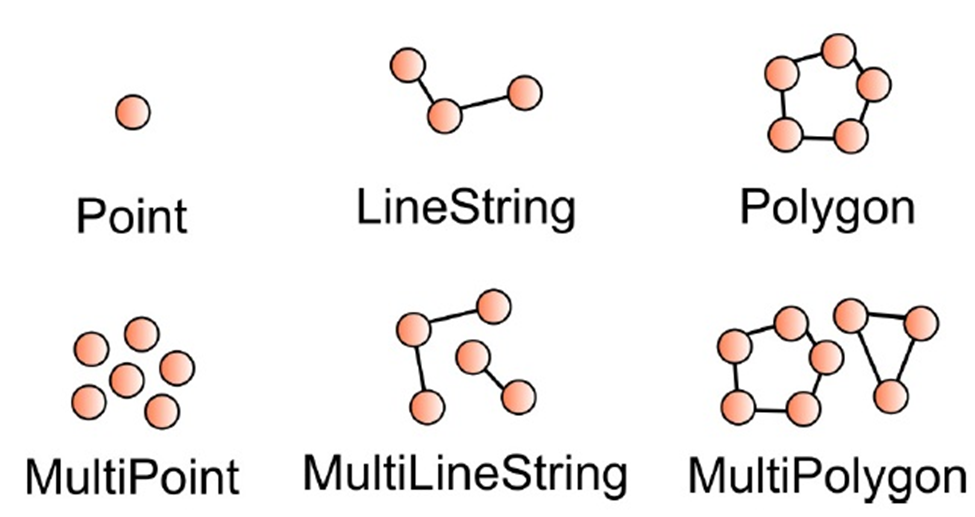
\includegraphics[width=1\linewidth]{data/sfs-sql}
			\caption{Tipos geométricos básicos suportados pela SFS-SQL. \cite{QUEIROZ_etal13}}
			\label{fig:sfs-sql}
		\end{figure}
		
		Além disso, a possibilidade na utilização da linguagem SQL com funções espaciais, permite que consultas espaciais sejam realizadas. O código a seguir, por exemplo, retorna todos os municípios do estado do Rio de Janeiro que estão a mais de 50km do aeroporto do Galeão:
		
		\begin{lstlisting}[float,floatplacement=H]
			SELECT municipio.nome
			FROM "nm.municip" As municipio, aeroporto_internacional As aeroint 
			WHERE st_DWithin(aeroint.geom, municipio.geom, 0.50) AND 
			aeroint.nome ILIKE "Galeao" AND
			municipio.uf ILIKE "RJ" AND
			municipio.nome NOT ILIKE "Rio de Janeiro"
		\end{lstlisting}
		
		Ou por exemplo, uma consulta para calcular o tamanho em quilômetros da rua "Douglas St." no município de Victoria pertencente ao estado do Texas?
		
		\begin{lstlisting}[float,floatplacement=H]
			SELECT sum(length(r.the_geom))/1000 AS kilometers
			FROM bc_roads r, bc_municipality m
			WHERE r.the_geom && m.the_geom
			AND r.name = "Douglas St"
			AND m.name = "VICTORIA";
		\end{lstlisting}
		
		Todas as consultas realizadas dentro de um SGBD podem ser optimizadas através do uso de mecanismos de indexação. Esses mecanismos servem para que o acesso ao dado requerido seja feito da forma mais rápida possível, excluindo a maior quantidade de dados não desejados em sua consulta. O PostGIS, o Oracle Spatial e o SpatiaLite optaram por utilizar o mecanismo de indexação baseado nas árvores-r (R-Tree) (GUTTMAN, 1984) Figura \ref{fig:arvorer}. Já o SQL Server e o IBM DB2 Spatial Extender utilizam o método por grades fixas multiníveis (Grid File) (NIEVERGELT et al., 1984)\cite{NIEVERGELT_etal84} e o space filling curves (LAWDER \& KING, 2000)\cite{LAWDER_KING} (QUEIROZ et. al., 2013)\cite{QUEIROZ_etal13}.
		
		\begin{figure}
			\centering
			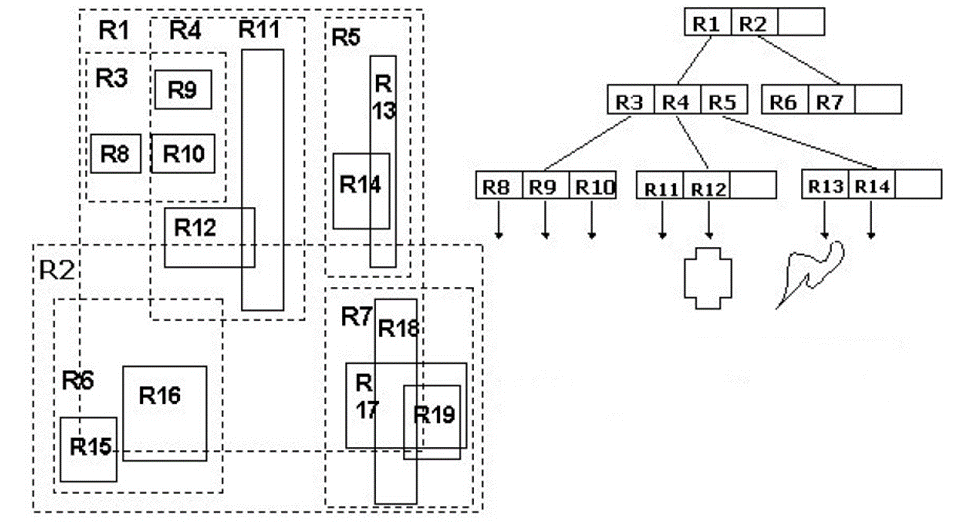
\includegraphics[width=1\linewidth]{data/arvore_r}
			\caption{Árvore-R. Modificado de Queiroz \& Ferreira (2006)}
			\label{fig:arvorer}
		\end{figure}
	
		Queiroz et. al. (2013)\cite{QUEIROZ_FERREIRA} nos mostra ainda que com o aumento da demanda, novas funcionalidades vem sendo desenvolvidas para tais sistemas. Um exemplo de inovação nessa área foi o desenvolvimento da extensão PostGIS Raster (OBE et. al., 2011)\cite{OBE_etal11} lançada em 2012, que possibilita diversas estratégias de armazenamento para imagens de sensoriamento remoto. Além disso, essa extensão permite o processamento de análises complexas envolvendo arquivos vetoriais e matriciais ao mesmo tempo. Além do PostGIS Raster, existem ainda projetos de desenvolvimento de extensões que visam solucionar problemas de representações topológicas como o PostGIS Topology ou de representações de rede como o pgRouting para o PostgreSQL e o Oracle Spatial Network Data Model (ORACLE, 2008)\cite{ORACLE}.
		
		Com o constante desenvolvimento de ferramentas e inclusão de funcionalidades nos SGBD-R, grande parte das aplicações que antes deveriam fazer necessariamente uso de um SIG, agora podem ser feitas diretamente do banco de dados. A vantagem disso é que assim, podemos ter um projeto, de fato, organizado e seguro. Além disso, o trabalho desenvolvido por Queiroz et. al. (2013)\cite{QUEIROZ_etal13} mostra que além dessas vantagens, a padronização deste tipo de suporte possibilitou o desenvolvimento de aplicativos geográficos interoperáveis e capazes de se integrar ao SGBD-R.
		
		O autor cita como exemplo bibliotecas de acesso de dados espaciais baseados em software livre como o GDAL (WARMERDAM, 2010)\cite{WARMERDAM}, GeoTools (TURTON, 2010)\cite{TURTON} e o TerraLib (CÂMARA et al., 2010)\cite{CAMARA_etal10}. SIGs para desktop como o Quantum GIS (QUANTUM GIS DEVELOPMENT TEAM, 2012)\cite{QGIS}, TerraView (CÂMARA et al., 2010)\cite{CAMARA_etal10} e o GRASS GIS (NETELER \& MITASOVA, 2008)\cite{NETELER_MITASOVA} tiveram um investimento visando a possibilidade de integração direta a SGBD-Rs e portanto, são capazes de visualizar e analisar diretamente os dados destes sistemas. Além disso, existe a possibilidade de integração com sistemas de disponibilização de serviço web para dados geográficos como os WMS ou Web Map Servers. WMS são ferramentas utilizadas para realizar a conexão entre o banco de dados onde seus mapas estarão armazenados e a camada de interface web. Podemos citar como exemplo o GeoServer (DAVIS, 2007)\cite{DAVIS_07}, um WMS feito em Java utilizando a ferramenta GeoTools (GEOTOOLS, 2016), o MapServer (KROPLA, 2005)\cite{KROPLA}, mais antigo e escrito em C, o TerraOGC (CÂMARA et al., 2010)\cite{CAMARA_etal10}. e o MapGuide (OSGEO, 2016), que possui API em PHP, .NET, Java e JavaScript. Outra opção mais moderna de servidor de mapas é o Mapnik (MAPNIK, 2016)\cite{MAPBOX_JS}. Suportado pela empresa Mapbox, o Mapnik é gratuito, livre e escrito em C++, possuindo versões de implementação em Python e mais recentemente em Node.js. Existem ainda projetos com soluções de menor porte como o PGRestAPI, também chamado de Chubbs Spatial Server (HAPSTER, 2016)\cite{HAPSTER} que utiliza Node.js para se conectar ao banco PostGIS.
		
		A utilização de servidores de mapas integrados a bancos de dados espaciais, em especial ao PostGIS vem se tornando cada vez mais popular principalmente devido as facilidades em que soluções como o Geoserver e o Mapnik para Node.js possuem de integração e configuração dos dados. Opções mais antigas e clássicas como o MapServer vem perdendo a preferência dos desenvolvedores para tais soluções. Inicialmente o MapServer perdeu usuários para o Geoserver. O Geoserver tem como base o Java e por consequência, uma interface de configuração mais intuitiva, além de uma maior portabilidade. Mas atualmente é o Geoserver que vem perdendo usuários. Uma das grandes apostas do mercado de geotecnologias atual é a utilização da linguagem JavaScript através do interpretador de código Node.js, que dá a possibilidade de utilizar JavaScript não somente para a construção de interfaces interativas com o usuário (\textit{frontend}), mas também no lado do servidor(\textit{backend}). Além das vantagens de se utilizar como base uma das linguagens mais difundidas e utilizadas em todo o planeta, Node.js dá a possibilidade de integração com bibliotecas escritas em C++ como o GDAL. Node.js possui ainda como uma das suas características principais a possibilidade de gerenciamento de conexões assíncronas/concorrentes, sendo uma ótima opção para soluções web que possuem um grande número de acesso. No entanto, não podemos dizer que seu rendimento no processamento de tarefas mais pesadas seja dos melhores. Sendo assim, sua utilização nem sempre pode ser a melhor das escolhas.
		
		Todo esse sistema de gerenciamento, armazenamento e disponibilização de dados ainda pode ser interligado adicionando uma última camada a estrutura de integração. Esta última camada utiliza aplicativos de visualização de dados geográficos para a web e depende de bibliotecas que dão a possibilidade de interligação deste tipo de dado aos browsers. Ferramentas como o OpenLayers (HAZZARD, 2011)\cite{HAZZARD}, o Google Maps API (DINCER \& URAZ, 2013\cite{DINCER_URAZ}; SVENNERBERG, 2010\cite{SVENNERBERG}; DUVANDER, 2010\cite{DUVANDER}), o Cesium (CESIUM, 2016)\cite{CESIUM}, o Microsoft Bing API (BING, 2016; DuVANDER, 2010\cite{DUVANDER}), o OpenStreetMap API (OSM, 2016)\cite{OSM}, o Tangram (TANGRAM, 2016)\cite{TANGRAM}, que renderiza mapas em 2D e 3D em tempo real no web \textit{browser} utilizando WebGL (MATSUDA \& LEA, 2013)\cite{MATSUDA_LEA},  assim como as soluções de PaaS (Platform as a Service) da Mapbox: Mapbox.js (MAPBOX A, 2016), sua implementação utilizando WebGL Mapbox.GL JS (MAPBOX B, 2016)\cite{MAPBOX_GLJS} e o Leaflet.js (LEAFLET, 2015)\cite{LEAFLET}, são exemplos de ferramentas fundamentais para que todo o processo de integração seja completo. Com esta estrutura, a divulgação de dados geográficos na web pode ser feita de fora organizada, segura e com um certo grau de interatividade entre o dado visualizado e o usuário final. É inquestionável que o desenvolvimento de ferramentas como estas possibilitaram uma grande evolução no modelo clássico de divulgação, onde o dado era disponibilizado de forma estática e não-integrada.
		
		Além de ferramentas ligadas a esta lógica de estruturação apresentada, SGBD-R geográficos ainda podem ser integrados diretamente a softwares de uso estatístico como o R (BIVAND et. al., 2013)\cite{BIVAND_etal13}, ou integrados a softwares \textit{desktop} utilizando linguagens de programação como Java (POSTGIS, 2015\cite{POSTGIS}; MARQUEZ, 2015\cite{MARQUEZ}), C\# (AGARWAL, 2012\cite{AGARWAL}; NPGSQL, 2016\cite{NPGSQL}) como no caso deste trabalho, Python, C, C++, e muitas outras. No entanto, é interessante lembrar que muitos SIG já possuem algum tipo de conectividade com SGBD. Trabalhos como o desenvolvido por Pimenta et. al. (2012), utilizam ferramentas de SIG como o Quantum GIS (QUANTUM GIS DEVELOPMENT TEAM, 2012)\cite{QGIS}, gvSIG (GVSIG, 2015)\cite{GVSIG} e SAGA (BÖHNER, 2006)\cite{BOHNER_etal06} para gerar informação em ambiente \textit{desktop}, transformar esta informação para um arquivo de formato suportado pelo MapServer, e finalmente gerar a visualização através do p.mapper (P.MAPPER, 2012)\cite{PMAPPER}. Ou trabalhos em que utilizam-se apenas um software SIG como o Quantum GIS, uma library como o Leaflet.js e um plugin como o Qgis2leaf para gerar e publicar mapas interativos online como é desenvolvido por Graser (2015)\cite{GRASER}. Ou utilizando o \textit{plugin} para QGIS desenvolvido pela Boundless chamado Web App Builder (BOUNDLESS, 2016). Ou seja, o uso dos softwares citados podem ser utilizados mas integrando-se somente algumas das partes.
		
		\subsection{Web arquiteturas de um mundo geográfico}
		
		A distribuição de mapas pela web nos dias atuais é feita de forma quase instantânea, independente de plataformas e da localização real dos usuários (IOSIFESCU, 2011)\cite{IOSIFESCU_11}. No entanto, esta distribuição vem sendo realizada através de sistemas especialistas desenvolvidos para realizar esta interação com o usuário da melhor forma possível, e não somente servindo como plataformas de distribuição de dados. Um desses sistemas web, e que será estudado neste capítulo, são os Sistemas de Informação Geográfica na web (SIG-Web) ou aplicativos de \textit{Web Mapping}. E para podermos entender melhor tal sistema, será necessário primeiramente entender a própria web e toda sua arquitetura sustentadora.
		
		Para começarmos, é importante entendermos que a internet é diferente da web. Internet é nada mais, nada menos, que uma rede de conexões entre computadores heterogêneos, ou não, interconectados por uma única tecnologia (TANENBAUM, 2002)\cite{TANENBAUM_02}. Atualmente, a tecnologia que possibilita esta interconexão é o protocolo TCP/IP. Já a web, é um sistema distribuído para troca de informações implementado sobre a internet. A web acaba servindo como uma forma de esquematizar, visualizar e interagir de uma forma mais organizada com o conteúdo armazenado e distribuído pela internet.
		
		É interessante lembrar que a web apresenta seus conteúdos através das URL (\textit{Uniform Resource Locator}). As URL, por sua vez, podem ser estáticas ou dinâmicas. O conteúdo estático é de fácil implementação mas tende a se tornar desatualizado mais rapidamente do que o dinâmico. Páginas web inteiramente escritas em HTML são um exemplo de conteúdo estático, já o conteúdo dinâmico, consegue gerar seu conteúdo de forma “\textit{on demand}”, ou seja, o conteúdo é gerado de acordo com as necessidades do usuário. Para isso, é necessário mais do que páginas em HTML, mas uma quantidade significativa de ferramentas e infraestrutura para prover todos os serviços e suportar a geração de todo o conteúdo (IOSIFESCU, 2011)\cite{IOSIFESCU_11}.
		
		O conteúdo na web é cada vez mais dinâmico. O aumento do poder computacional e de transmissão de dados, além da popularização de geotecnologias como o GNSS (\textit{Global Navigation Satellite System}) possibilitaram que os dados pudessem ser obtidos diretamente do campo, e não somente retirados de mapas impressos. Além disso, a implantação de sistemas GNSS em aparelhos móveis possibilitou que a obtenção de dados georreferenciados pudesse ser feita por qualquer usuário em qualquer lugar. Esta evolução contribuiu para que serviços de \textit{Web Mapping} ou \textit{Online Mapping Services} se tornassem cada vez mais populares e interativos. Atualmente, serviços online de distribuição de mapas como o Yahoo Maps (criado em 2002), Open Street Maps (2004), Google Maps (2005), Here (antigo OviMaps criado em 2007), Bing Maps (2008), ArcGis Online (2010), etc, buscam uma maior interação entre seus serviços e páginas web através do que Longley et al. (2011)\cite{LONGLEY_etal13} chama de \textit{mashup}. Além disso, existe um constante esforço de integração entre os serviços de distribuição online de mapas e Sistemas de Informa Geográfica comerciais (ArcGis, ERDAS, Global Mapper e Map Info, etc) e livres (Quantum Gis, Grass, GvSig, MapWindow, etc) (PIMENTA, 2011)\cite{PIMENTA}.
		
		Para entendermos melhor a GeoWeb e a até mesmo a criação de SIG-Webs, é crucial que possamos entender outros conceitos fundamentais. Um desses é o conceito de Arquitetura Orientada a Serviço, ou SOA (\textit{Service Oriented Architecture}). Arquiteturas Orientadas a Serviço são um estilo de arquitetura de software onde as funcionalidades implementadas por suas aplicações devem ser disponibilizadas através de serviços. Sendo assim, qualquer aplicação complexa pode ser decomposta em duas partes componentes, sendo cada uma delas distribuídas pela rede ou pela internet (LONGLEY et al. 2011)\cite{LONGLEY_etal13}. Este tipo de arquitetura é cada vez mais utilizado por possibilitar que aplicativos ou páginas web possam integrar serviços diferenciados em uma mesma interface. Esta integração facilita também a implementação de aplicações complexas que dependeriam do desenvolvimento de cada ferramenta em questão de forma separada, demandando uma quantidade enorme de mão de obra especializada, podendo restringir este tipo de aplicação a somente grandes empresas.
		
		Como já dito, toda esta arquitetura de desenvolvimento é baseada em serviços. Alonso et al. 2004, define serviços como uma parte de funcionalidade disponibilizado por um provedor de serviços a fim de entregar resultados para o usuário final (Figura \ref{fig:pedido-resposta}).
		
		\begin{figure}
			\centering
			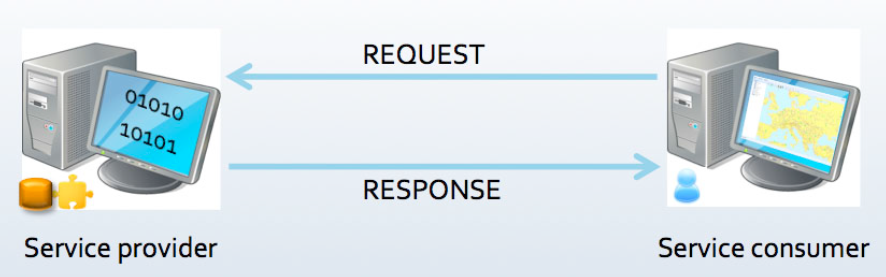
\includegraphics[width=1\linewidth]{data/pedido-resposta}
			\caption{Mecanismo de pedido – resposta. \cite{IOSIFESCU_11}}
			\label{fig:pedido-resposta}
		\end{figure}
		
		Além do conceito de serviço, a arquitetura orientada a serviço reforça a ideia de mensagem e interface. A comunicação com o usuário é feita através de mensagens. As mensagens por sua vez são entregues aos usuários por meio de interfaces. E as interfaces definem quais tipos de mensagens um serviço pode processar. Para todo esse sistema ser implementado de forma funcional, é necessário que exista uma série de padronizações. As mensagens são normalmente construídas utilizando arquivos XML (\textit{eXtensible Markup Language}). Atualmente, a transferências de mensagens pode ser realizada utilizando dois tipos de serviços web. A SOAP (\textit{Simple Object Access Protocol}) define o formato da mensagem e é normalmente utilizada junto a WSDL (\textit{Web Services Description Language}), que define a interface do serviço.  Ambas são linguagens XML com características diferentes que se complementam. Além disso, existe a REST (\textit{REpresentational State Transfer}), que surge como uma alternativa mais simples do padrão SOAP/WSDL. No entanto, grande parte do mercado prefere utilizar a alternativa SOAP/WSDL por ainda ter maior suporte da indústria e ser considerado o grande padrão na implementação de serviços web (IOSIFESCU, 2011)\cite{IOSIFESCU_11}.
		
		Além dos padrões de arquitetura, é necessário entender outros tipos de padronização que possibilitam que a interoperabilidade da GeoWeb. Os padrões web são desenvolvidos e geridos por organizações como a \textit{International Organization for Standardization} (ISO), a \textit{World Wide Web Consortium} (W3C), a \textit{Institute of Electrical and Electronics Engineers} (IEEE) ou a \textit{Open Geospatial Consortium} (OGC). A OGC é a responsável por manter e desenvolver padronizações de conteúdo e serviços na área geoespacial. Além da OGC, existe a \textit{Technical Committee} 211 (ISO/TC 211), formada pela ISO e pela própria OGC. A ISO/TC 211, por sua vez, serve para definir as estruturas de troca de dados geográficos.
		
		Algumas padronizações tiveram importância inquestionável na evolução na área de Geoinformação e da GeoWeb. Estes são a WMS (\textit{Web Map Server}), a SLD (\textit{Style Layer Descriptor}), a FES (\textit{Feature Encoding Specification}), a WFS (\textit{Web Feature Service}), a GML (\textit{Geography Markup Language}) e a SE (\textit{Symbology Encoding}).
		
		Dentre os padrões mais importantes, a WMS foi uma das primeiras a ser especificada. Criada em 2000 pela OGC, ela serviu para padronizar a forma como que clientes Web podiam realizar \textit{requests} de mapas padronizando não só o tipo de dado distribuído como seu metadado. A partir de 2005 a WMS passou a ser um padrão ISO internacional para serviços de mapa (ISO, 2005)\cite{ISO}.
		
		Dois anos depois, em 2002, mais quatro padrões foram especificados pela OGC: o \textit{Styled Layer Descriptor} (SLD) (OGC, 2002)\cite{OGC_02a}, o \textit{Filter Encoding Standard} (FES) (OGC, 2002b)\cite{OGC_02b}, a\textit{ Web Feature Service} (WFS) (OGC, 2002c)\cite{OGC_02c} e a \textit{Geography Markup Language} (GML) (OGC, 2002d)\cite{OGC_02d}. O SLD padroniza como a WMS pode ser estendida permitindo uma simbologia definida pelo usuário para dados de feições ou cobertura. Já o FES melhora a funcionalidade do WFS, do WMS e do SLD utilizando o XML. A OGC especificou também como o WFS e o GML funcionariam. O GML é nada mais do que uma codificação XML para modelar, transportar e armazenar funções básicas como a análise espacial de feições geográficas e não-geográficas. Já a especificação WFS define as interfaces de acesso de dado e operações de manipulação em feições geográficas utilizando o HTTP como protocolo de comunicação. O WFS e o GML são padrões bem interligados, já que o WFS permite o cliente enviar e receber dados espaciais em formato GML. E finalmente, em 2007, a padronização SE foi lançada, sendo assim uma continuação direta do antigo padrão SLD e se tornando a padronização mais recente elaborada pela OGC.
		
		A elaboração de padrões geoespaciais como os citados facilitam a troca de dados entre os SIG possibilitando que mesmo softwares privados utilizem uma mesma linguagem de comunicação em comum. O trabalho da OGC facilitou ainda que serviços online como os SIG Web, anteriormente baseados somente em padrões proprietários, pudessem interagir entre si e entre outros tipos de serviços. O sucesso desse esforço pode ser comprovado pela grande aceitação de padrões como o WFS e o SLD (IOSIFESCU, 2011)\cite{IOSIFESCU_11}.
		
		\subsection{A importância dos metadados}
		
		O crescimento tecnológico ao longo dos anos demonstrado até aqui, infelizmente não pode ser comparado a sua aplicação entre seus profissionais. A aplicação de metodologias ultrapassadas ainda é um problema na área geotecnológica. Um dos grandes problemas, e que será analisado neste capítulo, é a pouca utilização e importância dada aos metadados.
		
		Metadados são modelos de representação ou abstração dos dados, com o objetivo de descrever e identificar as características (MOURA, 2005)\cite{MOURA}. A utilização de metadados é relevante por servir justamente de fonte para qualquer tipo de informação sobre o dado no qual se esta trabalhando. São dados sobre dados.
		
		Sendo assim, o objetivo dos metadados na geoinformação é o de sistematizar o armazenamento de dados espaciais facilitando não só o funcionamento de bases de dados e seu gerenciamento de informações, mas aos próprios SIGs, caso contrário, o acesso as informações se tornam muito mais demoradas, complexas e sujeitas a erros. O aumento significativo na distribuição de dados digitais georreferenciados maximiza ainda mais a necessidade da utilização de metadados. Informações como: autoria, escala, sistema de projeção, tipo de armazenamento, etc, são informações essenciais para um trabalho cartográfico bem realizado, e portanto, indispensavelmente presentes em arquivos de metadado.
		
		Alguns SIGs geram o arquivo de metadado de forma automática com pelo menos um mínimo de informação (autor, data, sistema de coordenada, datum e escala), apesar disso, para uma boa distribuição e utilização de arquivos metadado, é sugerido que se tenha ao menos elementos como Moura (2005)\cite{MOURA} nos mostra:
		
		\begin{itemize}
			\item Autor, data da elaboração e registro de atualizações
			\item Metodologia de construção do dado
			\item Formato de armazenamento (matricial ou vetorial)
			\item Fonte do dado, escala da fonte e ano da fonte
			\item Resolução (em caso de arquivo matricial) e Padrão de Exatidão Cartográfica
			\item Sistema de projeções e coordenadas, datum horizontal e vertical
			\item Extensões disponíveis e aplicativo utilizado
			\item Conteúdo das camadas de informação
			\item Georreferência (coordenadas do retângulo envolvente) e área de mapeamento
			\item Informações específicas sobre grades utilizadas, equidistância de pontos na representação de algumas feições geométricas, entre outros.
			\item Demais informações gerais específicas sobre o dado.
		\end{itemize}
		
		\subsection{Avanços em SIG Web e cartografia orientada à serviços web}
		
		A organização de dados georreferenciados em bancos de dados espaciais como o PostGIS possibilita que o analista encontre alternativas de implementação de sistemas que contribuem não somente na análise dos dados como em sua distribuição na web. Sendo assim, se torna cada vez mais comum a implementação de SIG Webs e projetos de\textit{ Web Mapping} que vise uma maior configuração de acordo com o uso específico de cada projeto. O avanço significativo nas tecnologias envolvidas neste tipo de implementação se dá pela aplicação de linguagens de programação que visem tornar esses sistemas cada vez mais complexos e interativos. É relativamente normal encontrar sistemas cartográficos web baseados na geração de informação interativa à partir de bancos de dados geográficos e não somente à partir de dados georreferenciados estáticos que visam somente a visualização dos mesmos.
		
		Com o tempo, linguagens de programação orientadas a objeto começaram a ser utilizadas para o desenvolvimento desses sistemas. Dentre elas, a de maior utilização é sem dúvida o Java. Java é uma linguagem orientada a objeto que se difundiu entre a comunidade de programadores por ser multiplataforma e ter a possibilidade de interligar aplicações originalmente offline a web. Dentro das geotecnologias a linguagem Java é igualmente importante, tendo grande aplicação cartográfica na web por sua possibilidade de implementação ligando banco de dados geográficos como o PostgreSQL/PostGIS a softwares especialistas.
		
		A Aplicação do Java como uma linguagem de programação ligada a aplicações geotecnológica vem sendo discutida por autores como Iosifescu (2013)\cite{IOSIFESCU_13}, onde vários de seus pontos positivos e negativos são demonstrados. A natureza multiplataforma da linguagem e sua interatividade com serviços web foram indiscutivelmente uma de suas maiores vantagens em relação a outras linguagens orientadas a objeto como o C\#. O C\#, por ter sido uma linguagem desenvolvida pela Microsoft, possuiu durante muito tempo a limitação de só poder ser utilizada e com todas as suas funcionalidades e integrada a ferramentas dependentes do sistema operacional Windows. Isso gerou uma consequente preferência entre os desenvolvedores ligados ou não a área de geotecnologia pela linguagem Java. 
		
		No entanto, Iosifescu (2013)\cite{IOSIFESCU_13} cita algumas complicações relacionadas ao uso da linguagem Java. Sua interação com sistemas de banco de dados geográficos requer a aplicação de funções SQL dentro do código fonte Java, gerando problemas de compilação no código final. Apesar de muitas vezes o código fonte Java estar correto e sem falhas graves, o compilador Java não percebe erros relacionados a sintaxe SQL por uma falta de integração entre as ferramentas.
		
		\begin{figure}
			\centering
			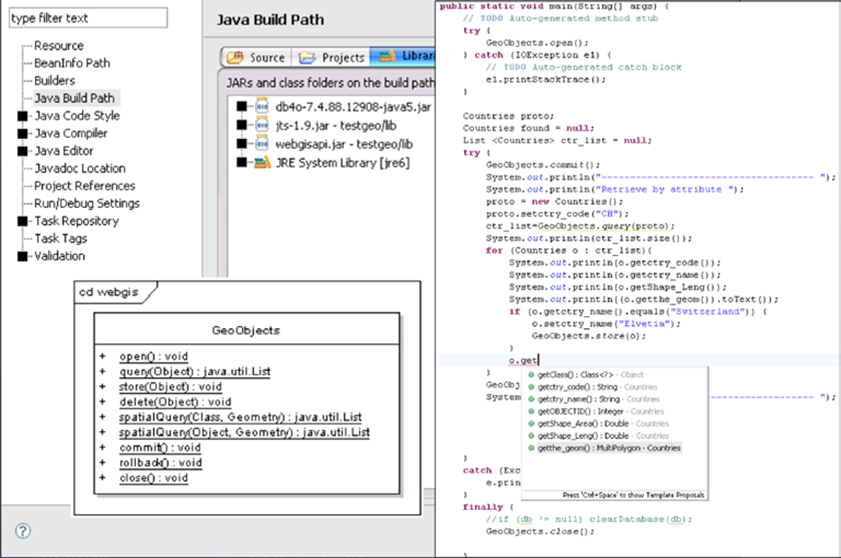
\includegraphics[width=1\linewidth]{data/sigweb_developer_side}
			\caption{O lado da programação no desenvolvimento de SIG Webs. (IOSIFESCU, 2009)}
			\label{fig:sigwebdeveloperside}
		\end{figure}
	
		\begin{figure}
			\centering
			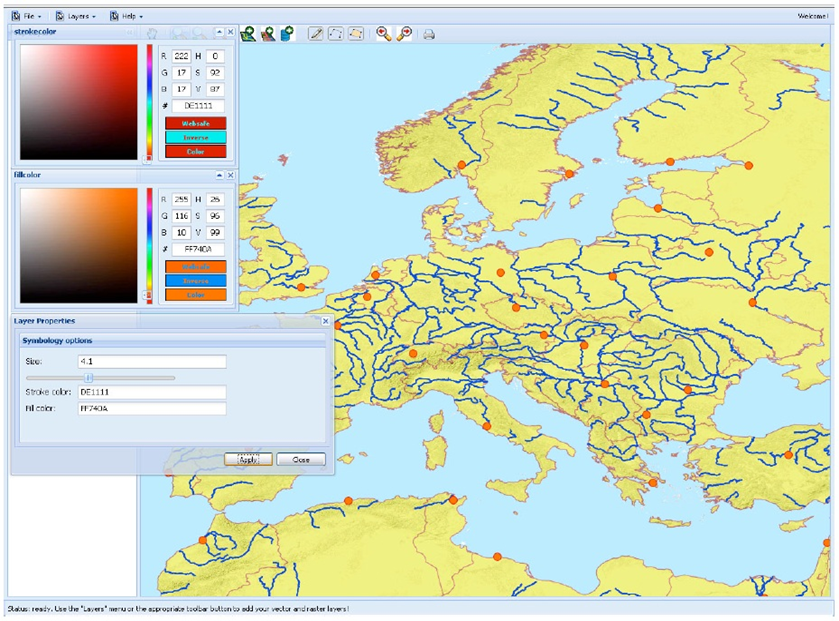
\includegraphics[width=1\linewidth]{data/sigweb_cartografico_side}
			\caption{O lado cartográfico do desenvolvimento SIG Web. (IOSIFESCU, 2009)}
			\label{fig:sigwebcartograficoside}
		\end{figure}
		
		No entanto, grande parte do desenvolvimento atual de SIG Webs ainda se baseia na estruturação de modelos pré-desenvolvidos com ferramentas de Web Mapping como o OpenLayers (PEREZ, 2012)\cite{PEREZ}, que foi desenvolvido em JavaScript e permite que o usuário faça pré-definições no código configurando-o a suas necessidades, mas limitando-se a modificações mais complexas. A opção pelo desenvolvimento de um SIG Web, assim como qualquer aplicação cartográfica na Web, ou utilizando-se de ferramentas de \textit{Web Mapping} pré-desenvolvidas, envolve muitas variáveis. A primeira é a disponibilidade de pessoas suficientemente treinadas para programar em linguagens de nível médio como o Java. O desenvolvimento de um sistema inteiro depende de um conhecimento sólido tanto em lógica de programação como na sintaxe de cada linguagem utilizada no processo. Além disso, é necessário um tempo de planejamento e desenvolvimento muito maior do que os que utilizam APIs (\textit{Application Programming Interface}). A escolha pela implementação de plataformas Web Mapping é normalmente uma opção de grande parte dos pesquisadores, já que tais sistemas muitas vezes atendem as necessidades atuais dos mesmos. 
		
		Por outro lado, a utilização de linguagens como Java e C\# ainda são essenciais por possuírem um desempenho maior do que linguagens de \textit{script} voltadas para a web. A importância de pensar no desempenho está principalmente no tempo de resposta que o aplicativo possui, deixando todo o processo mais fluido. O processo de análise de dados espacializados, assim como no processo de renderização dos mapas requer um maior processamento, sendo assim, linguagens compiladas possuem clara vantagem sobre as voltadas a web, por serem interpretadas.
		
		Apesar do Java ter reinado como uma das principais linguagens de programação utilizadas na área geotecnológica nos últimos anos, a recente abertura da linguagem C\# pela Microsoft, assim como sua extensa utilização pela comunidade de desenvolvedores através das plataformas Xamarin (recentemente adquirida pela Microsoft) e da \textit{engine} Unity, sua popularidade mudou e tende a mudar ainda mais nos próximos anos (Figura \ref{fig:rankinggithub}).
		
		\begin{figure}
			\centering
			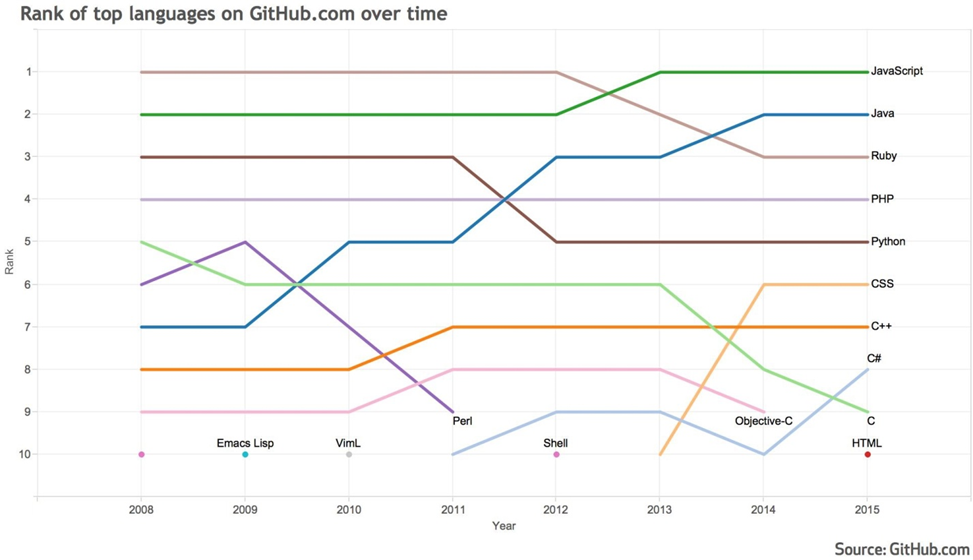
\includegraphics[width=1\linewidth]{data/ranking_github}
			\caption{Ranking das linguagens de programação com maior quantidade de projetos na plataforma GitHub.}
			\label{fig:rankinggithub}
		\end{figure}
		
		Mesmo não sendo linguagens voltadas ao desenvolvimento web, não só o Java quanto o C\# possui como característica a produção de aplicações que se comunicam pela web com interfaces voltadas para o desenvolvimento "\textit{frontend}" como o OpenLayers e Leaflet, fornecendo a parte "\textit{backend}" do serviço. Sendo assim, é possível desenvolver aplicações geoespaciais com suporte a padrões como o WFS e o WMS que servem não somente como uma interface de manipulação desses dados como também na distribuição do conteúdo gerado e utilizando para a internet. Sendo assim, a dualidade entre as tecnologias SIG Web utilizadas atualmente depende de variáveis diretamente ligadas aos objetivos de cada projeto.
		
		\subsection{Interatividade e cartografia digital na web}
		
		A adoção de aplicações e serviços web, assim como a de \textit{smartphones} e sua integração com o GNSS promoveram uma verdadeira revolução cartográfica. A visualização de mapas digitais estáticos evoluiu não só esteticamente, mas também na quantidade de informação apresentada. Os mapas clicáveis surgiram como uma alternativa de maior interatividade na web, demonstrando que a cartografia não necessariamente precisa ser restrita apenas ao que se vê de forma estática, mas apresentando conteúdo de acordo com os interesses do usuário final. O desenvolvimento da cartografia digital não parou por ai no entanto. 
		
		Atualmente, as maiores inovações na cartografia digital se dão quando ligadas ao conceito de interatividade. Grandes bases de dados geográficas são criadas visando a implementação de sistemas onde o usuário passa a montar seu mapa de acordo com o conteúdo oferecido. Sistemas de Gerenciamento de Banco de Dados Objeto Relacional (SGBDOR) como o PostgreSQL/PostGIS através da linguagem SQL (\textit{Structured Query Language}) passam a ser implementados e integrados a sistemas desenvolvidos para a web possibilitando que consultas sejam feitas e até mesmo adicionadas a base.
		
		A necessidade de interagir com o mapa nunca foi tão grande. O que era considerado estático e de certa forma esquecido passou a ser utilizado massivamente no cotidiano de grande parte da população mundial. O usuário não quer apenas obter informações do mapa, ele quer contribuir, ele quer adicionar informação a base de dados. A colaboração do usuário se torna de extrema importância para que aplicações funcionem de forma devida. A colaboração do usuário passa a ser o centro da questão, ao invés de apenas mais uma possibilidade.
		
		Como consequência, a quantidade de informação espacial e sua difusão é cada vez maior, sendo assim, organizá-las da melhor forma possível para um melhor uso é essencial. Este tipo de informação não pode ser mais tratada como um tipo de informação adicional ou excepcional, mas sim como um tipo de informação crítica, sendo necessário cada vez mais confiabilidade e interatividade. Grande parte da evolução tecnológica atual e das últimas décadas convergiu para que a informação geográfica fosse cada vez mais difundida e interativa, e o futuro não se mostra diferente. Este é um futuro inevitável. 
		
		\subsection{Tecnologias Web}
		
		A internet armazena dados espaciais desde seu início. No entanto, grande parte das tecnologias desenvolvidas durante toda sua história não solucionaram problemas de visualização que impossibilitavam o usuário final de manusear um mapa com pelo menos algum nível de interatividade. Por muito tempo os usuários finais tinham acesso apenas a mapas estáticos ou com muitas limitações de interação. Esse tipo de problema se deu pela estrutura na qual os serviços web foram desenvolvidos e pela própria história evolucionária da internet. 
		
		Principalmente a partir do final da década de 2000, a internet passou a incorporar ferramentas desenvolvidas para receber e armazenar dados dos usuários de forma constante, o que consequentemente significou uma transformação na forma com que esse usuário interagisse com esses serviços. Este usuário passou não só a receber uma quantidade ainda maior de informação, mas também a conceder mais dados e a interagir com serviços que antes seriam inimagináveis.
		
		Antes, com uma internet baseada em serviços mais estáticos, seria impensável um usuário ter a disposição \textit{websites} onde pudesse interagir com mapas com diferentes níveis de zoom, escalas e dados plotados de acordo com o nível de abstração. Essa limitação se dava or vários motivos. Primeiramente, o desenvolvimento de um serviço como esse necessitaria do uso de diversas linguagens de programação como HTML, ASP.Net, Python, PHP, além de uma quantidade realmente grande de dados armazenados no servidor. Toda a estrutura deveria ser desenvolvida a partir do zero, necessitaria de um corpo especialista com bons conhecimentos em programação e, mesmo que bem implementado, teria uma grande chance de sofrer com a falta de desempenho, já que estaria utilizando ferramentas de finalidade genérica não-otimizadas para este tipo de uso. Sobre essas limitações, Obe et. al. (2011)\cite{OBE_etal11} possui uma passagem explicativa:
		
		\begin{quote}
			"... These interface features would all require extensive programming on the client side. If server-side programming didn’t already discourage the GIS specialist, the client-side programming surely will. What we need is a suite of client tools with useful controls for map viewing and editing already built. Sure, the suite will dictate the overall appearance and functionality, but this still is preferable to building our own solution from the ground up. After all, our goal is to disseminate our maps, not to program web servers..."
		\end{quote}
	
		Como OBE et. al. (2011)\cite{OBE_etal11} fala em seu trabalho, a solução para tais problemas seria o desenvolvimento de ferramentas de uso específico que facilitariam a visualização de dados geográficos na internet. Tais ferramentas foram de fato foram desenvolvidas com o tempo e possibilitam que muitos dos dados que antes eram de difícil acesso e manuseio pelo grande público, fizesse parte cada vez mais da vida dessas pessoas. Pode se dizer que o sucesso no uso de ferramentas desse tipo para a distribuição de dados geográficos na internet se dá pelo uso dos servidores de mapas (\textit{Mapping Servers}).
		
		\subsubsection{Mapping Servers (Servidores de mapa)}
		
		Servidores de mapa servem principalmente para um propósito: servir como renderizador de imagens e entregar ao cliente estas informações em tempo real. Um servidor web convencional nunca seria capaz de fazer o que um servidor de mapas faz porque dentro de em uma estrutura convencional, um mapa seria fornecido apenas se tal dado existisse previamente no servidor. Para armazenar um mapa com diversos níveis de zoom em um servidor web convencional, seria necessário que o mesmo armazenasse todos os níveis de forma individualizada, multiplicando o mapa em diversas imagens e consumindo seu poder de armazenamento e de processamento. Já no servidor de mapas, a mesma imagem seria gerada somente quando o pedido fosse feito pelo usuário final, economizando recursos (OBE et. al., 2011)\cite{OBE_etal11}.
		
		Atualmente os servidores de mapas mais utilizados são o MapServer, o GeoServer, o FeatureServer (FEATURESERVER, 2015)\cite{FEATURESERVER} e o SharpMap.NET (SHARPMAP, 2015)\cite{SHARPMAP}. A escolha pela plataforma correta deve ocorrer de acordo com as necessidades do projeto desenvolvido pelo especialista. A Figura \ref{fig:prerequisitosmappingservers} nos mostra os pré-requisitos de cada plataforma:
		
		\begin{figure}
			\centering
			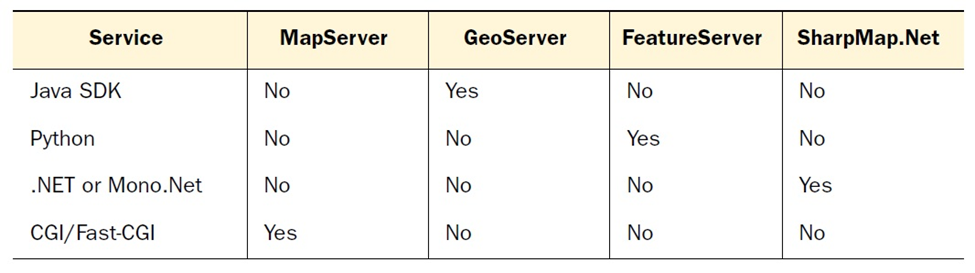
\includegraphics[width=1\linewidth]{data/prerequisitos_mapping_servers}
			\caption{Pré-requisitos dos principais servidores de mapa. \cite{OBE_etal11}}
			\label{fig:prerequisitosmappingservers}
		\end{figure}
		
		O FeatureServer e o SharpMap.NET são as opções menos populares, com menor quantidade de recurso e com maior dificuldade de configuração. No entanto, estas soluções são utilizadas em alguns casos devido a vantagens específicas de cada um. O SharpMap.NET, por exemplo, garante vantagens ao desenvolvedor .NET devido a sua maior integração com a plataforma. Já o FeatureServer tem como vantagem ser escrito totalmente em Python e ter sido desenvolvido originalmente para funcionar de forma integrada com o OpenLayers. 
		
		O MapServer, diferente dos dois citados, é extremamente popular e possui diversas vantagens. Primeiramente ele pode ser executado sem a necessidade de instalação, desde que utilize seus arquivos de configuração em qualquer outro servidor web tradicional. Além disso, possui uma API (\textit{Application Programming Interface}) chamada MapScript, que possibilita o desenvolvimento de ferramentas utilizando linguagens de programação como PHP, Python e C\#. No entanto, o MapScript possui a disvantagem de não possuir um ambiente de configuração agradável como os que utilizam CGI (Common Gateway Interface). Toda a configuração do MapServer deve ser portanto, configurada através de arquivos "Mapfile" como o exemplificado a seguir (KROPLA, 2005)\cite{KROPLA}: 
		
		\begin{lstlisting}[float,floatplacement=H]
			01  # This is our first mapfile
			02  NAME "First"
			03  SIZE 400 300
			04  IMAGECOLOR 255 255 255
			05  IMAGETYPE JPEG
			06  SHAPEPATH "/home/mapdata/"
			07  EXTENT -125.00 20.00 -65.00 50.00
			08  WEB
			09      TEMPLATE '/var/www/htdocs/first.html'
			10      IMAGEPATH '/var/www/htdocs/tmp'
			11      IMAGEURL '/data/tmp/'
			12  END
			13  LAYER
			14      NAME "US States"
			15      STATUS default
			16      TYPE line
			17      DATA "statesp020"
			18      LABELITEM "STATE"
			19      CLASS
			20          STYLE
			21              COLOR 0 0 0
			22      END
			23      LABEL
			24              COLOR 0 0 0
			25              SIZE SMALL
			26          END
			27      END
			28  END
			29  END
		\end{lstlisting}
		
		Por último temos o GeoServer. O GeoServer é desenvolvido em Java e possui um \textit{web server} próprio chamado Jetty. Além disso, possui a grande vantagem de ter um ambiente gráfico de configuração como mostrado da Figura \ref{fig:geoservergui}, e integração direta com o OpenLayers. O GeoServer é considerado o servidor de \textit{Web Mapping} mais fácil de ser configurado e possui provavelmente o maior crescimento dentre os aplicativos citados aqui. Trabalhos como o de Bartolomeoli (2014)\cite{BARTOLOMEOLI}, Garnett, et. al. (2014)\cite{GARNETT_etal15}, Giannecchini (2013)\cite{GIANNECCHINI}, Kwun (2014)\cite{KWUN}, Aime (2014)\cite{AIME}, Kunicki (2013)\cite{KUNICKI}, Garnett \& Aime (2014)\cite{GARNETT_AIME} e Hansen (2014)\cite{HANSEN} demonstram bem esta evolução.
		
		\begin{figure}
			\centering
			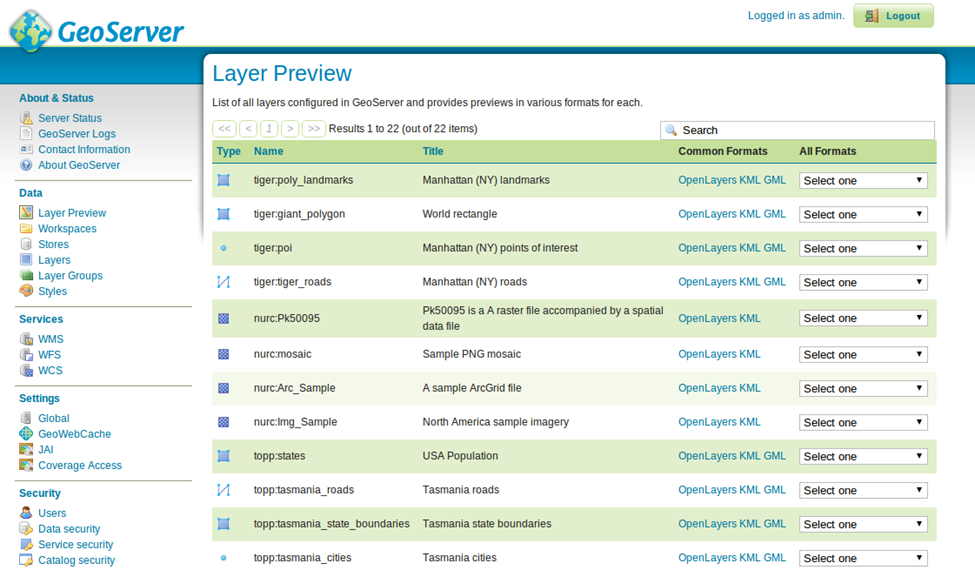
\includegraphics[width=1\linewidth]{data/geoserver_gui}
			\caption{Ambiente gráfico de configuração do GeoServer}
			\label{fig:geoservergui}
		\end{figure}
	
		O GeoServer é também, o único servidor de mapas a possuir compatibilidade a todos os principais padrões de \textit{web service} da OGC como o WMS (Web Mapping Service), WFS (Web Feature Service) e WFS-T (Web Feature Service Transactional) como mostra a Figura \ref{fig:suportewebservices}.
		
		\begin{figure}
			\centering
			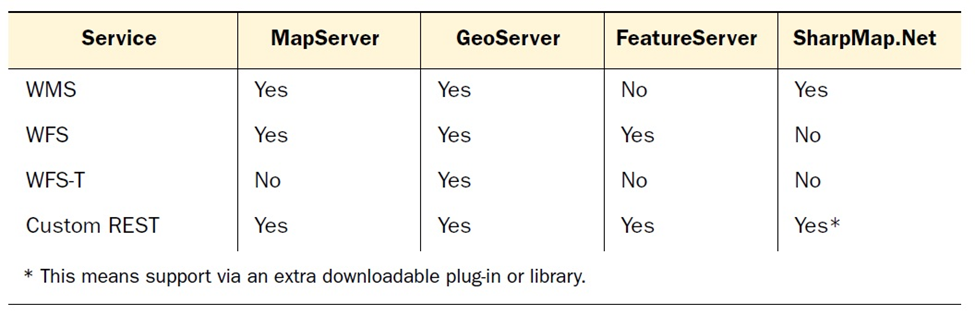
\includegraphics[width=1\linewidth]{data/suporte_webservices}
			\caption{Suporte a web services. \cite{OBE_etal11}}
			\label{fig:suportewebservices}
		\end{figure}
		
		Os serviços padronizados pela OGC são de extrema importância para o funcionamento de um servidor de mapas. Existem basicamente três tipos de padrão de serviços que se diferenciam em algumas características. O WMS (\textit{Web Mapping Service}), por exemplo, permite que o servidor possa renderizar dados do tipo vetor e \textit{raster} para arquivos de imagem do tipo JPEG, PNG, TIFF e outros. Este processo de transformação do dado é realizado no lado do servidor primeiramente porque seria dificultoso transmitir dados geográficos brutos pela internet, e segundo, porque grande parte dos usuários finais encontrariam dificuldades em processar os dados em dispositivos como \textit{smartphones}. O segundo padrão é o WFS (\textit{Web Feature Service}). Este padrão tem a função de gerar dados de saída do tipo vetor usando arquivos do tipo XML (\textit{eXtensible Markup Language}) como GML (Geography Markup Language), KML (\textit{Keyhole Markup Language}) ou até mesmo Geo-JSON (\textit{Geography JavaScript Object Notation}). É uma ferramenta interessante para desenvolvedores que utilizam JavaScript em seus projetos e é o melhor serviço para ser utilizado para usuários que desejam adicionar layers de informação com atributos. O WFS é normalmente utilizado em conjunto ao WMS, onde o WMS é responsável pela renderização de imagens em pequena escala cartográfica (sem zoom), e o WFS ao tornar o mapa mais detalhado ao utilizar o zoom, mostrando informações mais detalhadas. Por último existe ainda o WFS-T \textit{(Web Feature Service Transactional}), que serve como um padrão para que os servidores de mapas possibilitem ao usuário de serviços web e \textit{desktop} a opção de editar dados vetoriais sem ter, de fato, acesso ao banco de dados (OBE et. al., 2011)\cite{OBE_etal11}. 
		
		Protocolos de serviços com o WMS, WFS, WFS-T e até mesmo o REST - \textit{Representational state transfer} (versão mais leve do WFS) permitem que dados de tipos diferentes sejam acessados por uma única interface web. Portanto, é importante sabermos exatamente que tipo de dados e compatibilidade com bases de dados cada servidor de mapas possui. A Tabela \ref{fig:compatibilidadeformatos} mostra a relação de compatibilidade entre cada um dos \textit{web-mapping servers} e os principais banco de dados espaciais. É bom notar que todos os servidores de mapa possuem compatibilidade com geometrias do PostGIS e arquivos \textit{shapefile} da ESRI (OBE et. al., 2011)\cite{OBE_etal11}.
		
		Nos últimos dois anos outras opções de ferramentas também se destacaram principalmente pelo constante desenvolvimento e amadurecimento de novas linguagens e bibliotecas. Um desses exemplos é o Mapnik, software de código livre desenvolvido pela Mapbox. O Mapnik é uma \textit{toolkit} de ferramentas voltadas para o desenvolvimento de aplicações geoespaciais que também possui a funcionalidade de um servidor de mapas quando utilizado junto a outras soluções. Além disso, com o desenvolvimento de linguagens modernas como Python e Node.js, as implementações de soluções espaciais na web ficam cada vez mais acessíveis. Antes, grande parte do processo de desenvolvimento dependia da programação de sistemas com linguagens mais complexas como C++, mas com o surgimento e o amadurecimento de linguagens como Node.js, o trabalho de implementação de um servidor passa a ser muito mais simples por ter a possibilidade de ser todo desenvolvido em JavaScript, por exemplo. Além disso, muitas das ferramentas geoespaciais já consolidadas como GDAL, e até mesmo o próprio Mapnik, estão ganhando versões mais simplificadas utilizando Node.js e Python principalmente. Esta simples transição de linguagens significa na prática uma grande mudança, já que transforma uma ferramenta antes utilizada apenas por poucos especialistas em uma ferramenta com capacidade de manipulação utilizando-se de linguagens mais populares, sendo assim por consequência mais acessível e rápida de ser entregue. 
		
		\begin{figure}
			\centering
			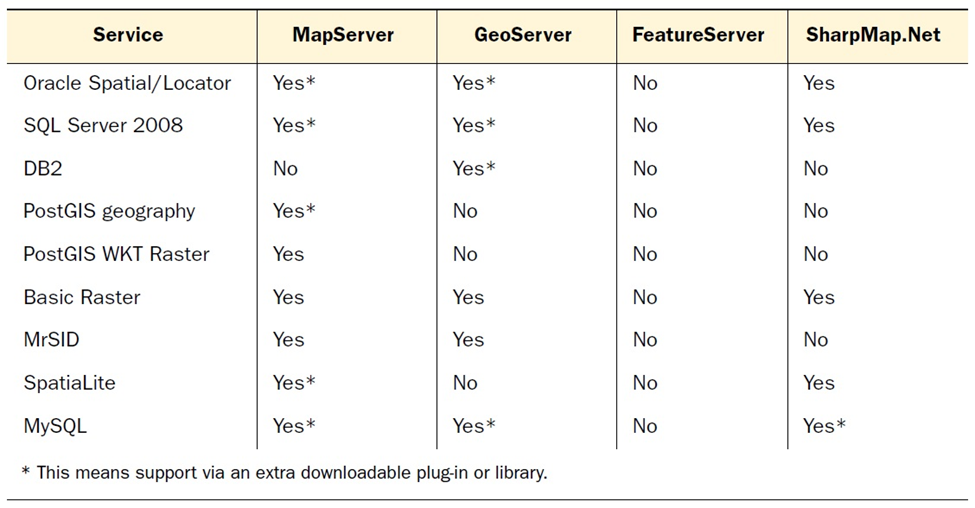
\includegraphics[width=1\linewidth]{data/compatibilidade_formatos}
			\caption{Compatibilidade entre formatos de fonte de dados.\cite{OBE_etal11}}
			\label{fig:compatibilidadeformatos}
		\end{figure}
		
		Outra possibilidade de desenvolvimento de um servidor de mapas é utilizando ferramentas como o DotSpatial. Assim como o SharpMap.Net, o DotSpatial é voltando para o desenvolvimento de soluções em C\#. A ferramenta possui por padrão diversas outras ferramentas de análise espacial como em qualquer outro SIG, mas dando a possibilidade de reutilização do código de forma única de acordo com o desenvolvimento realizado. Também possui acesso os principais banco de dados espaciais e a grande maioria dos formatos \textit{raster} e vetoriais por utilizar uma extensão da biblioteca GDAL para a manipulação dos dados.
		
		\subsubsection{Mapping Clients}
		
		Após a configuração do servidor de mapas, é necessário a criação de uma última camada dentro dessa estrutura espacial integrada: a interface com o usuário. Os \textit{mapping clients} são necessários para receber a informação do servidor e enviá-la ao usuário final através de uma interface \textit{web} ou \textit{desktop}.
		
		Muitas aplicações \textit{desktop} são compatíveis com os padrões OGC e conseguem interagir de forma integrada aos dados armazenados no banco de dados e gerados pelo servidor de mapas. Muitos SIG \textit{open source} como o Quantum GIS, uDIG, gvSIG, OpenJUMP ou privados como o ArcGIS Desktop, MapInfo, entre outros, são capazes de realizar tal integração. Esta integração pode ser feita utilizando toda a estrutura (banco de dados geográfico - sistema de informação geográfica - servidor de mapa - aplicação web), como pode ser ligado diretamente apenas a algumas dessas aplicações. Apesar dos problemas de compatibilidade, muitos SIG como o ArcGIS já possuem ligação direta a aplicações web para a publicação direta de projetos na internet. Este tipo de escolha tem feito cada vez mais a cabeça dos especialistas em geotecnologia, já que a divulgação e visualização de dados geográficos na internet vem se tornando cada vez mais comum. Além disso, é bom lembrar que com o desenvolvimento de ferramentas integração o esforço técnico envolvido neste processo diminui, possibilitando inclusive que especialistas em geotecnologia sem maior treinamento em programação sejam capazes de criar aplicativos geográficos interativos na web.
		
		Estas aplicações web são muitas vezes programadas em Ajax e em uma mistura de linguagens de \textit{script}. Atualmente, ferramentas como a Leaftlet e o OpenLayers são as ferramentas web mais utilizadas e com um maior grau de desenvolvimento. O OpenLayers se destaca ainda por ter compatibilidade com os padrões OGC e com formatos fora do padrão. Além disso, possui compatibilidade com \textit{toolkits} como o GeoExt, um \textit{framework} JavaScript que combina o OpenLayers com Extjs  e transforma a interface em um ambiente mais parecido com um SIG \textit{desktop} (OBE et. al., 2011)\cite{OBE_etal11}.
		
		O desenvolvimento do OpenLayers é todo baseado na linguagem JavaScript, possuindo uma boa comunidade e documentação online. Com isso, muitos trabalhos vem sendo publicados utilizando cada vez mais aplicativos de \textit{web mapping}, especialmente com o desenvolvimento do OpenLayers 3 (SCHAUB, 2014\cite{SCHAUB}; LEMOINE, 2014\cite{LEMOINE}). Todas suas novas configurações, ferramentas e funções mais utilizadas estão disponibilizadas de forma gratuita no próprio \textit{website} do desenvolvedor. Sendo assim, aplicações das mais diversas natureza são exemplificadas com acesso direto ao seu código-fonte como podemos ver na Figura \ref{fig:openlayers}: 
		
		\begin{figure}
			\centering
			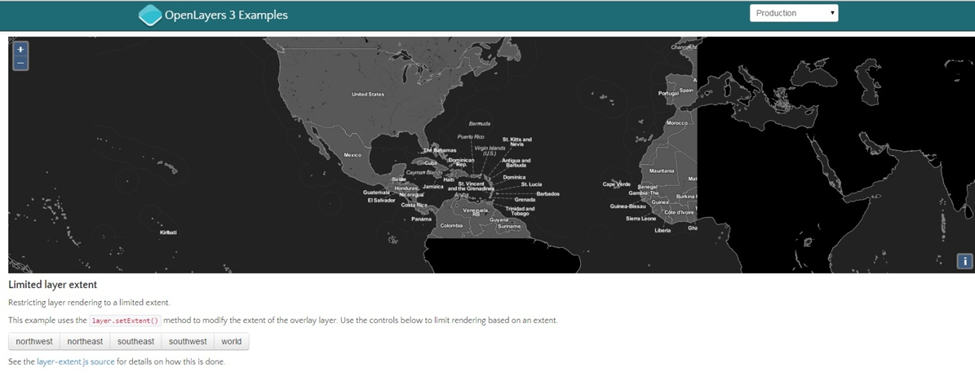
\includegraphics[width=1\linewidth]{data/openlayers}
			\caption{Exemplo presente no \textit{website} oficial do OpenLayers 3 demonstrando como carregar layers limitando sua extensão.}
			\label{fig:openlayers}
		\end{figure}
		
		O código para o exemplo é disponibilizado à seguir: 
		
		\begin{lstlisting}
			function transform(extent) {
				return ol.proj.transformExtent(extent, 'EPSG:4326', 'EPSG:3857');
			}
			
			var extents = {
				northwest: transform([-180, 0, 0, 85]),
				northeast: transform([0, 0, 180, 85]),
				southeast: transform([0, -85, 180, 0]),
				southwest: transform([-180, -85, 0, 0]),
				world: transform([-180, -85, 180, 85])
				};
				
				var base = new ol.layer.Tile({
					source: new ol.source.TileJSON({
					url: 'http://api.tiles.mapbox.com/v3/' +
					'mapbox.world-black.jsonp',
					crossOrigin: 'anonymous'
					})
				});
				
				var overlay = new ol.layer.Tile({
					extent: extents.northwest,
					source: new ol.source.TileJSON({
					url: 'http://api.tiles.mapbox.com/v3/' +
					'mapbox.world-glass.jsonp',
					crossOrigin: 'anonymous'
					})
				});
				
				var map = new ol.Map({
					layers: [base, overlay],
					renderer: exampleNS.getRendererFromQueryString(),
					target: 'map',
					view: new ol.View({
					center: [0, 0],
					zoom: 1
					})
				});
				
				for (var key in extents) {
				document.getElementById(key).onclick = function(event) {
				overlay.setExtent(extents[event.target.id]);
			};
		}
		\end{lstlisting}
		
		Além de aplicativos de \textit{web mapping open source} como o OpenLayers e o Leaflet, o mercado oferece ainda opções privadas como o Google Maps, Bing e MapQuest. Obe et al. (2011)\cite{OBE_etal11}, e nos mostra que tais soluções foram essenciais para a popularização de mapas interativos pela internet por serem desenvolvidas de forma integrada e por possuírem uma interface de fácil uso. Com o tempo, serviços como o Google Maps Engine surgiram dando a possibilidade de edição através de APIs JavaScript. No entanto, tais ambientes de desenvolvimento ainda se mostram limitados por não permitirem utilizar \textit{querys} SQL, adicionar dados externos mais complexos e, modificar ferramentas existentes assim como sua exclusão são tarefas complicadas. 
		
		
	
	\part{Metodologia}
	\chapter{Materiais e métodos}

A construção de um SIG, assim como o ato de pensar a modelagem de dados é uma tarefa complexa, não somente pela sua característica intelectual abstrata, como também por sua complexidade técnica. 

A longo da evolução computacional dos últimos 30 anos, o processamento e visualização de dados espaciais sofreram mudanças significativas no uso de algoritmos geoespaciais como vimos no capítulo anterior. A popularização de tais técnicas possibilitaram que sua implementação fosse realizada em diversas linguagens de programação, incluindo linguagens mais populares e de nível de abstração mais alto como Python. A compilação de algoritmos em bibliotecas voltadas para o processamento de dados espaciais como GDAL, Mapnik, SharpMap.Net, DotSpatial, Orfeo ToolBox, assim como a criação de interfaces de desenvolvimento a SIG consagrados como o ArcPy e o PyQGIS, possibilitaram que o desenvolvimento de sistemas de tratamento de dados georreferenciados fosse feito de forma mais prática, rápida e eficiente. 

A consequência dessa evolução é a possibilidade de criação de softwares especialistas para determinados tipos de estudos ou serviços, sejam eles aplicativos \textit{closed} ou \textit{open source}. Pela natureza de código aberto dos projetos citados, a consequência é que parte dos projetos que envolvam tais bibliotecas também acabem sendo projetos \textit{open source}. Além disso, acabam sendo bastante utilizadas no meio acadêmico e dão a possibilidade que trabalhos como este possam ser realizados.

Para este trabalho, houve uma escolha política pela priorização do uso de software livre. Esta escolha foi tomada primeiramente pela grande capacidade de uso dessas ferramentas por praticamente qualquer usuário com acesso mínimo a um computador básico e conexão a internet. Desprezando-se a complexa relação entre a interface gráfica e o usuário, o que por si só engloba algumas áreas de estudo do conhecimento humano, pode se dizer que a utilização de software livre na Geografia, assim como em toda a academia, facilita o processo de replicação. É importante lembrar que a escolha por ferramentas livres, principalmente no ato de fazer ciência em um contexto político e econômico como o caso brasileiro, se torna essencial quando possível. 

O segundo motivo pela utilização de soluções livres se deu pela grande capacidade técnica dessas ferramentas, o que prova o grau de maturidade não somente de seus projetos, mas também da comunidade em relação a importância do uso e do suporte que tais aplicações necessitam. 

Outra vantagem importante no uso dessas tecnologias é o alto grau de compatibilidade e integração que elas oferecem. Grande parte dos SIG e software de PDI (Processamento Digital de Imagens) proprietários atualmente resistem à ideia de liberar a documentação necessária para que seja facilitada a integração de ferramentas (extensões) e software externos a sua própria interface. Empresas como a ESRI, famosa pelo desenvolvimento do pacote ArcGIS prefere oferecer os recursos de integração de dados espaciais e armazenamento em banco de dados geográficos em parceria a softwares de natureza igualmente proprietária como o Microsoft SQL Server desenvolvido pela Microsoft. No entanto, justamente por não oferecer os recursos necessários para qualquer tipo de desenvolvedor externo, o software não oferece a possibilidade de integração total (leitura e escrita) com a extensão PostGIS, assim como para outros projetos. Este tipo de problema de compatibilidade ainda é bastante comum entre as ferramentas de geoprocessamento e sensoriamento remoto, já que grande parte do uso de softwares na área ainda se dá pela utilização de soluções proprietárias. No entanto, grande parte das ferramentas \textit{open source} da área e que vem sendo desenvolvidas nos últimos anos tem solucionado este grande problema. O aumento de compatibilidade e a integração, são características do desenvolvimento de ferramentas\textit{ open source} como um todo, e na área de geotecnologias não vem sendo diferente.

Todas as ferramentas escolhidas para a realização deste trabalho possuem a vantagem de possuir uma grande quantidade de desenvolvedores competentes envolvidos e em constante atividade nos respectivos projetos. Além disso, são projetos que muitas vezes se complementam em seus avanços, facilitando a aplicação de novas soluções não somente em uma das partes, mas em todas as partes envolvidas. É importante ainda dizer que serão utilizadas as últimas versões dos softwares em questão, e que o lançamento de novas versões dos mesmos tende a ser mais rápida que as das soluções proprietárias, já que o desenvolvimento é descentralizado e constante.

\section{Motivações técnicas para a utilização do PostGIS}

A escolha pelo uso do PostGIS se deu também pelo fato da ferramenta possuir algumas características técnicas que não se encontram em opções proprietárias como o ArcSDE/Geodatabase da ESRI. Apesar de popularmente ser conhecido como um banco de dados espacial, o Geodatabase não pode ser classificado como um banco de dados, mas sim como uma ferramenta de gerenciamento.

O PostGIS possui ainda como diferencial a forma com que o dado espacial é inserido e gerenciado, possuindo diferenças fundamentais das utilizadas pelas ferramentas distribuídas pela ESRI. O ArcSDE da ESRI gerencia na verdade todos os processos entre o cliente e o banco, armazenando os dados espaciais em formato genérico BLOB, o que faz com que o banco de dados seja utilizado através de suas funcionalidades mesmo não “entendendo” que o dado é na verdade espacial. De certa forma, o aplicativo desenvolvido por este trabalho cria uma interface com o banco de dados PostGIS de uma forma similar ao que o ArcSDE faz com o Microsoft SQL Server. Sendo assim, não podemos entender o Geodatabase como um banco de dados por sí só, mas uma interface de conexão com outros bancos que nem sempre reconhecem tipos de dados espaciais de forma nativa.

Um banco de dados geográficos nativamente ativado consegue tratar o dado espacial armazenado de forma diferente de um dado comum. A vantagem disso é a possibilidade de se utilizar métodos de consulta, indexação e análise específicos para dados geográficos. Ou seja, o banco de dados geográficos entende que o dado armazenado possui uma localização, influenciando diretamente e principalmente nas consultas em SQL.

Sendo assim, podemos listar algumas das vantagens e das desvantagens de se utilizar uma interface administrativa como o ArcSDE em relação a um DBMS geográfico, assim como a utilização de arquivos \textit{shapefile} como opção de armazenamento de dados geográficos: \\

\textbf{Vantagens ao utilizar arquivos Shapefile:}

	\begin{itemize}
		\item É o tipo de arquivo mais utilizando na área geotecnológica. Possui ampla compatibilidade.
		\item É um formato de arquivo relativamente fácil de se trabalhar, principalmente por iniciantes na área.
	\end{itemize}
		
\textbf{Desvantagens dos arquivos Shapefile:}

	\begin{itemize}
		\item Não possui a capacidade de armazenar informações topológicas dos dados.
		\item Não possui suporte para a criação de \textit{splines}. Sendo assim, feições mais suaves só podem ser representadas por polígonos, deixando o tamanho do arquivo muito maior que o normal, já que o número de pontos de conexão tende a aumentar de acordo com o maior detalhamento da escala.
		\item Tanto os arquivos .shp como os .dbf não podem ultrapassar o tamanho de 2GB (231 bytes), uma média de 70 milhões de pontos.
		\item Os arquivos .dbf baseados no antigo padrão dBase não permitem tabelas com mais que 255 colunas e com nomes limitados a apenas 10 caracteres. 
		\item O arquivo .dbf possui ainda uma limitada quantidade de tipos de dado. O formato suporta apenas dados de tipo ponto flutuante (\textit{float}) com tamanho máximo de apenas 13 caracteres, números inteiros (\textit{integer}) de 9 caracteres, tipo data (date) com máximo de 8 caracteres e texto (\textit{text}) de apenas 254 caracteres.
		\item Números de ponto flutuante (\textit{float}) podem conter erros de redundância, já que são na verdade armazenados como do tipo texto (\textit{text}).
	\end{itemize}

\textbf{Vantagens de se utilizar o Geodatabase:}

	\begin{itemize}
		\item Excelente integração com outros produtos ESRI
		\item Boa performance
		\item Controle de versões implementado nativamente
	\end{itemize}

\textbf{Desvantagens de se utilizar o Geodatabase:}

	\begin{itemize}
		\item Recuperar dados corrompidos pode ser complicado
		\item A licença de uso é ligada ao banco de dados
		\item Complicações ao acessar geometrias fora do ambiente de softwares desenvolvidos pela ESRI
		\item A edição de dados espaciais por mais de um usuário ao mesmo tempo é possível apenas em sua versão mais sofisticada
	\end{itemize}

\textbf{Vantagens de se utilizar o PostGIS:}

	\begin{itemize}
		\item Capacidade de fácil integração a aplicações externas utilizando consultas SQL
		\item Solução gratuita e de código livre
		\item Utilização de formatos abertos
		\item Excelente performance quando utilizado em conjunto a outras soluções geoespaciais como o QGIS e o Geoserver (ANDERSON \& DEOLIVEIRA, 2007)
		\item Pode ser administrado utilizando ferramentas de backup, análise e restauração já bastante conhecidas e utilizadas na área de banco de dados.
		\item A possibilidade de consultas utilizando SQL pode ser vantajosa caso a administração do banco seja feita por alguém que possua conhecimento técnico, mesmo que este conhecimento seja somente na administração de banco de dados convencionais.
		\item A possibilidade de edição de dados espaciais por mais de um usuário ao mesmo tempo vem habilitada por padrão.
	\end{itemize}

\textbf{Desvantagens de se utilizar o PostGIS:}

	\begin{itemize}
		\item A necessidade da utilização da linguagem SQL pode ser uma desvantagem dependendo do conhecimento técnico da equipe que utilizará o sistema.
		\item Apesar de existir opções externas, falta um sistema de controle de versões nativo.
	\end{itemize}
	
	\part{Resultados e Considerações Finais}
	\chapter{Resultados}
\section{Modelagem dos dados utilizando OMT-G}
A princípio, os dados utilizados para a elaboração do trabalho já existiam como resultado de uma tese defendida pelo Prof. Dr. Vinícius da Silva Seabra, atual professor adjunto da Faculdade de Formação de Professores, campus vinculado à Universidade do Estado do Rio de Janeiro. A parti da geração desses dados, Seabra (2012) realizou um estudo geossistêmico da BHRSJ (Bacia Hidrográfica do Rio São João) buscando classificar a bacia em grupos de paisagem dando importância as características sistêmicas através da manipulação de dados bióticos, abióticos e socioeconômicos. O trabalho apresenta assim as características da bacia de forma que possamos visualizar áreas mais e também menos propícias à recuperação ambiental.

A partir da aquisição desses dados, o processo de modelagem conceitual do banco de dados foi necessário para que pudéssemos pensar a estrutura do banco antes de sua real implementação. O processo de abstração se deu utilizando o modelo OMT-G desenvolvido por Davis (2000). O banco de dados em questão será geográfico, sendo assim, a opção pelo uso de um modelo como o OMT-G se deu primeiramente por seguir as primitivas baseadas em objeto partindo da lógica utilizada pelo modelo UML e segundo, por possuir primitivas de diagramação baseadas na natureza geográfica dos objetos modelados, aumentando a capacidade semântica dos dados.

O modelo OMT-G organizado para este trabalho (Figura \ref{fig:modeloomt-gfinal}) se baseou em diagramas elaborados por Seabra (2012)\cite{SEABRA}, e foi todo desenvolvido utilizando uma ferramenta disponibilizada pelo próprio Departamento de Ciência da Computação da Universidade Federal de Minas Gerais. A ferramenta é gratuita, possui código aberto disponibilizado pela plataforma GitHub (https://github.com/lizardoluis/omtg-designer) e pode ser utilizada através do endereço http://www.aqui.io/omtg/. A ferramenta é toda estruturada na web e possui a funcionalidade de exportar o modelo criado pelo usuário diretamente em código SQL compatível com bancos de dados Oracle e PostGIS, além da possibilidade de salvar o próprio modelo em arquivos XML para possíveis alterações.

O trabalho realizado por Seabra foi organizado utilizando diversos diagramas com o objetivo de mostrar a produção, processamento e organização dos dados necessários para a realização de um estudo de favorabilidade. Utilizando-se o modelo OMT-G, há a possibilidade da criação de apenas um diagrama integrador, levando em consideração suas características semânticas e dando a possibilidade de exportação direta para bancos de dados espaciais.

Toda esta etapa de implementação foi importante por demonstrar que apesar da complexidade esperada ao se criar modelos de dados conceituais do ambiente, a criação de estruturas computacionais complexas, assim como sua etapa de implementação vem se tornando cada vez mais acessível a usuários não especializados.  Por final, espera-se que a modelagem e implementação sirva como um sistema de suporte a decisão não só para estudos de favorabilidade na bacia do rio São João, mas para diversos outros estudos com o mesmo tema.

	\afterpage{\clearpage}
	\begin{sidewaysfigure}[ht]
		\centering
		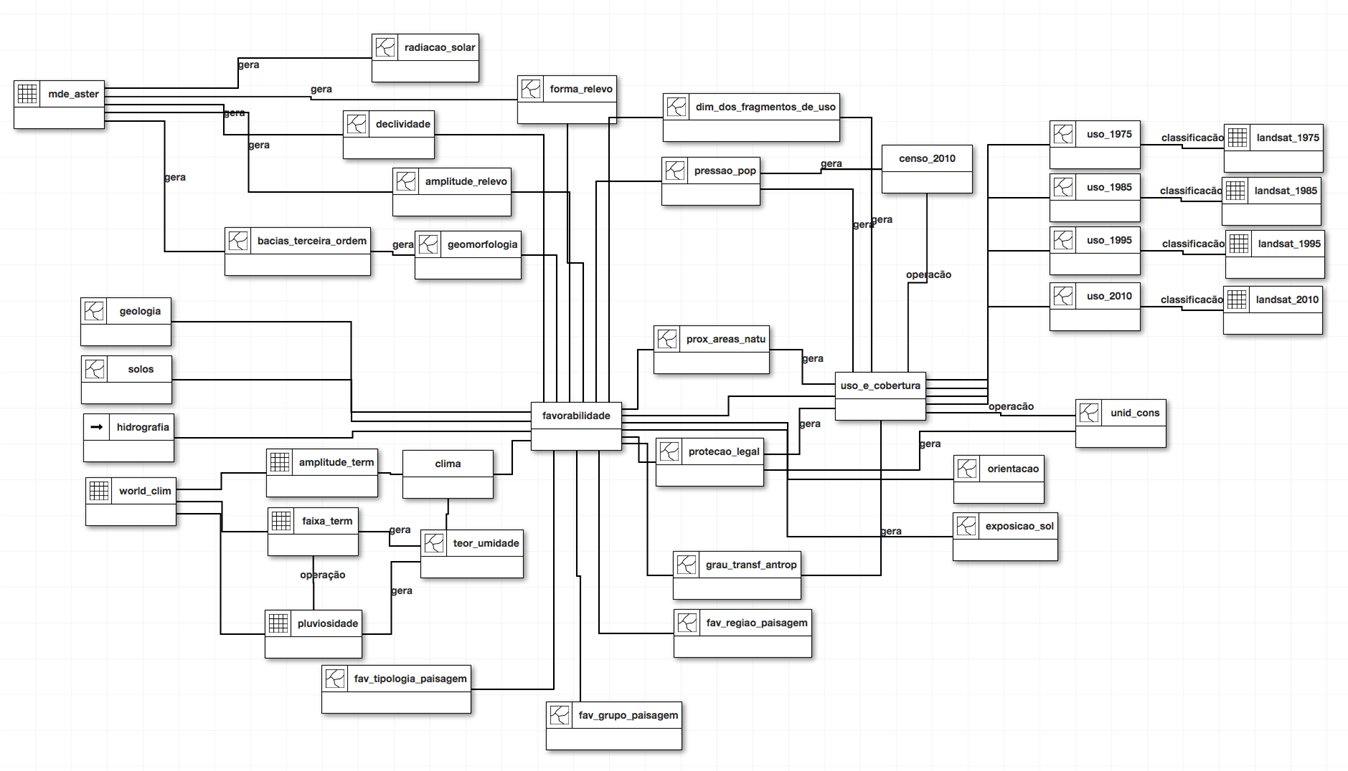
\includegraphics[width=1\linewidth]{data/modelo_OMT-G_final}
		\caption{Modelo OMT-G baseado no estudo realizado por Seabra (2012)\cite{SEABRA} na BHRSJ.}
		\label{fig:modeloomt-gfinal}
	\end{sidewaysfigure}

\newpage
\section{Implementação do modelo no PostGIS}

O banco de dados geográfico foi implementado utilizando o Sistema Gerenciador de Banco de Dados Objeto Relacional (SGBDOR) PostgreSQL versão 9.5 (64-bit) utilizando-se a extensão espacial PostGIS versão 2.2.2, assim como a interface gráfica pgAdmin versãoIII (Figura \ref{fig:pgadmin-gui}). 

	\begin{figure}
		\centering
		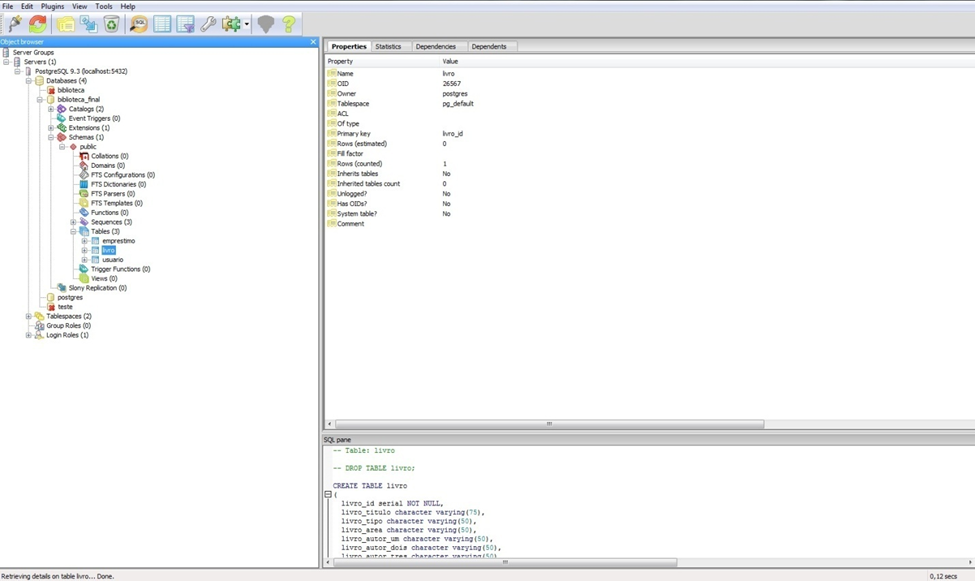
\includegraphics[width=1\linewidth]{data/pgAdmin-gui}
		\caption{Interface gráfica pgAdmin III utilizada para gerenciar o SGBDOR PostgreSQL assim como a extenção espacial PostGIS}
		\label{fig:pgadmin-gui}
	\end{figure}

A etapa de implementação do modelo OMT-G no banco PostGIS é relativamente rápida e simples. Através do pgAdmin podemos criar um novo banco de dados (Figura \ref{fig:newdbpgadmin}).

	\begin{figure}
		\centering
		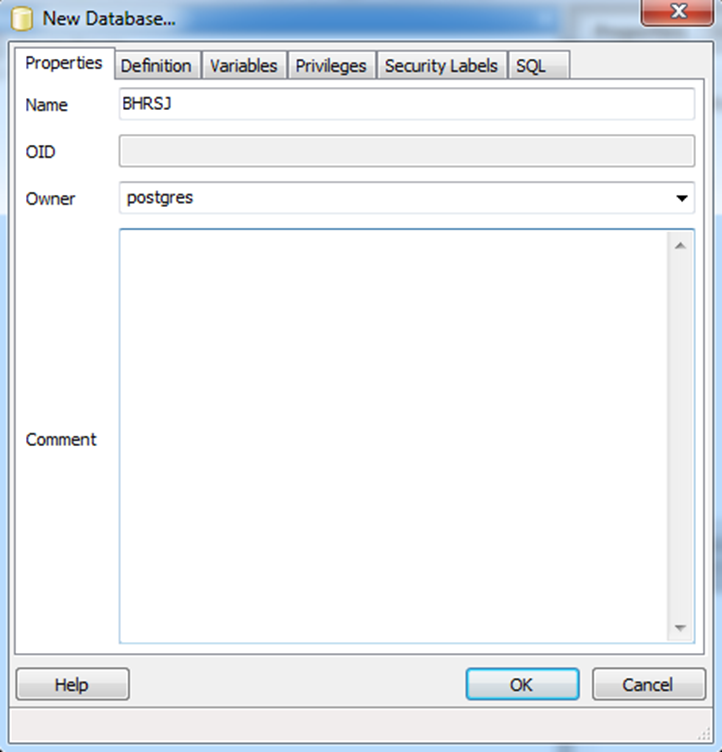
\includegraphics[width=0.6\linewidth]{data/newdb_pgadmin}
		\caption{Janela de criação de bancos no PostgreSQL 9.5 utilizando a interface pgAdmin III.}
		\label{fig:newdbpgadmin}
	\end{figure}
	
Após este processo, devemos dizer ao banco recém criado que gostaríamos de utilizar a extensão espacial PostGIS, ou seja, devemos dizer ao banco que queremos transformá-lo em um banco geográfico através de uma consulta SQL. A princípio, a ideia de adicionar a extensão espacial PostGIS através de uma consulta SQL pode parecer estranha, mas é o único método possível. Outras extensões com o \textit{pgRouting}, \textit{PostGIS Topology}, \textit{Point Cloud}, o módulo \textit{raster}, assim como outros, podem ser adicionados em um único comando:

	\begin{minipage}{\linewidth}
	\begin{lstlisting}
		CREATE DATABASE BHRSJ;
		\connect BHRSJ;
		-- Inicia a extensao PostGIS (ja inclui o modulo raster)
		CREATE EXTENSION postgis;
		-- Inicia a extensao Topology
		CREATE EXTENSION postgis_topology;
		-- Inicia a extensao PostGIS Advanced 3D 
		-- assim como outros algoritmos de geoprocessamento
		-- Inicia as extensoes relacionadas a geocoding
		CREATE EXTENSION postgis_sfcgal;
		CREATE EXTENSION fuzzystrmatch;
		CREATE EXTENSION address_standardizer;
		CREATE EXTENSION address_standardizer_data_us;
		CREATE EXTENSION postgis_tiger_geocoder;
		-- Inicia a extensao pgRouting para trabalhos que utilizam analise de rota
		CREATE EXTENSION pgrouting;
		-- Inicia a extensao pgr_fdw para adicionar outros tipos de dados externos
		CREATE EXTENSION ogr_fdw;
		
		-- Suporte para dados de LIDAR
		CREATE EXTENSION pointcloud;
		CREATE EXTENSION pointcloud_postgis;
	\end{lstlisting}
	\end{minipage}

No entanto, nem sempre é necessário adicionar todas as extensões em todos os projetos. Grande parte dos projetos, assim como este, utilizam apenas o módulo principal, iniciado através do comando "CREATE EXTENSION postgis;" (Figura \ref{fig:createextensionpostgis}). Após a execução deste comando, o PostgreSQL criará automaticamente uma tabela em seu banco nomeada "spatial ref sys" contendo o número de identificação de todos os 3911 códigos EPSG representando os sistemas de referência catalogados pela \textit{International Association of Oil and Gas Producers}. No Brasil, alguns códigos EPSG são mais utilizados do que outros, como o 4326 (WGS 84), o 4618 (SAD 69) e o 4674 (SIRGAS 2000)

	\begin{figure}
		\centering
		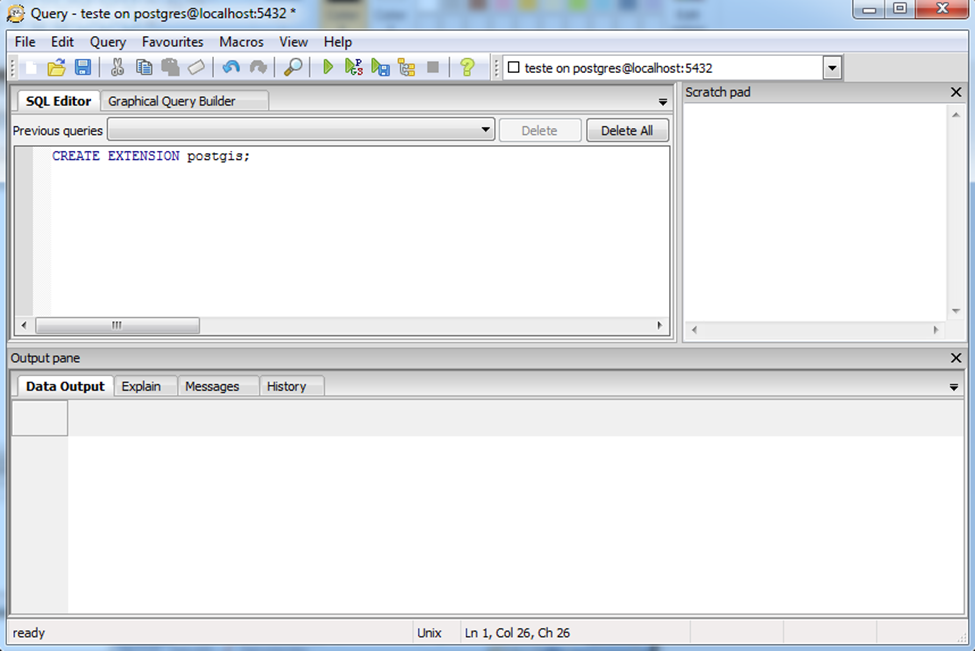
\includegraphics[width=1\linewidth]{data/create_extension_postgis}
		\caption{Através da consulta "\textbf{create extension postgis}" o banco recém-criado já poderá utilizar as funcionalidades espaciais.}
		\label{fig:createextensionpostgis}
	\end{figure}

Após a etapa de criação do banco e da inicialização da extensão PostGIS, inicia-se a etapa de importação de todos os dados definidos a serem inclusos pela nossa modelagem OMT-G. A importação de dados georreferenciados é diferente das importações de simples tabelas. Para esta etapa utilizamos um \textit{plugin} chamado PostGIS Shapefile and DBF Loader 2.1 (Figura \ref{fig:shapefileloader}). Nas últimas versões instaladas através do instalador oficial, o \textit{plugin} de importação de \textit{shapefiles} já vem incluso e instalado por padrão, sendo ainda mais fácil de importar dados em formato \textit{shapefile}. Para a importação de dados georreferenciados em outros formatos é necessário a utilização de outros \textit{plugins} como osm2pgsql que importa dados derivados do projeto OpenStreetMap para o PostGIS. Caso o plugin não esteja funcionando ou não o tenha instalado ainda é possível adicionar \textit{shapefiles} utilizando o Prompt de Comando e a ferramenta shp2pgsql e adicionando e executando o arquivo .sql criado na ferramenta de consultas SQL do pgAdmin:

	\begin{lstlisting}[float,floatplacement=H]
		shp2pgsql -s SRID shapefile.shp nome_da_tabela > shapefile.sql
	\end{lstlisting}

	\begin{figure}
		\centering
		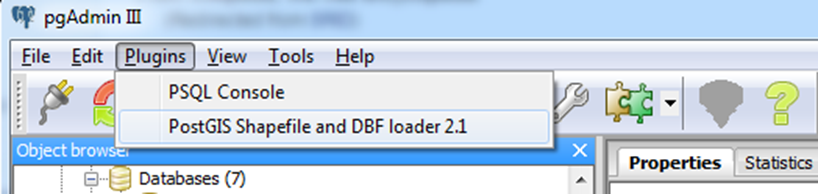
\includegraphics[width=1\linewidth]{data/shapefile_loader}
		\caption{Shapefile and DBF Loader 2.1.}
		\label{fig:shapefileloader}
	\end{figure}
	
Ao utilizar a interface gráfica do \textit{plugin} é importante que se configure o SRID (\textit{Spatial Reference System Identifier}) de cada \textit{shapefile} adicionado (Figura \ref{fig:shapefileloadergui}). É possível também adicionar múltiplos \textit{shapefiles} e/ou arquivos .dbf ao mesmo tempo. Além disso, é provável que seja necessário configurar a codificação do arquivo .dbf adicionado de OTF-8 para LATIN1 caso a tabela de atributos do \textit{shapefile} adicionada contenha caracteres típicos da linha portuguesa (Figura \ref{fig:importconfig}).

Outra funcionalidade da ferramenta de importação é a possibilidade de executar os algoritmos de indexação espacial como o GiST (\textit{Generalized Search Tree}) por padrão, já na etapa de importação e sem a necessidade de executar comandos SQL, como o demonstrado a seguir por exemplo:
	
	\begin{lstlisting}[float,floatplacement=H]
		CREATE INDEX nome_da_tabela_gix ON nome_da_tabela USING GIST (the_geom);
	\end{lstlisting}

	\begin{figure}
		\centering
		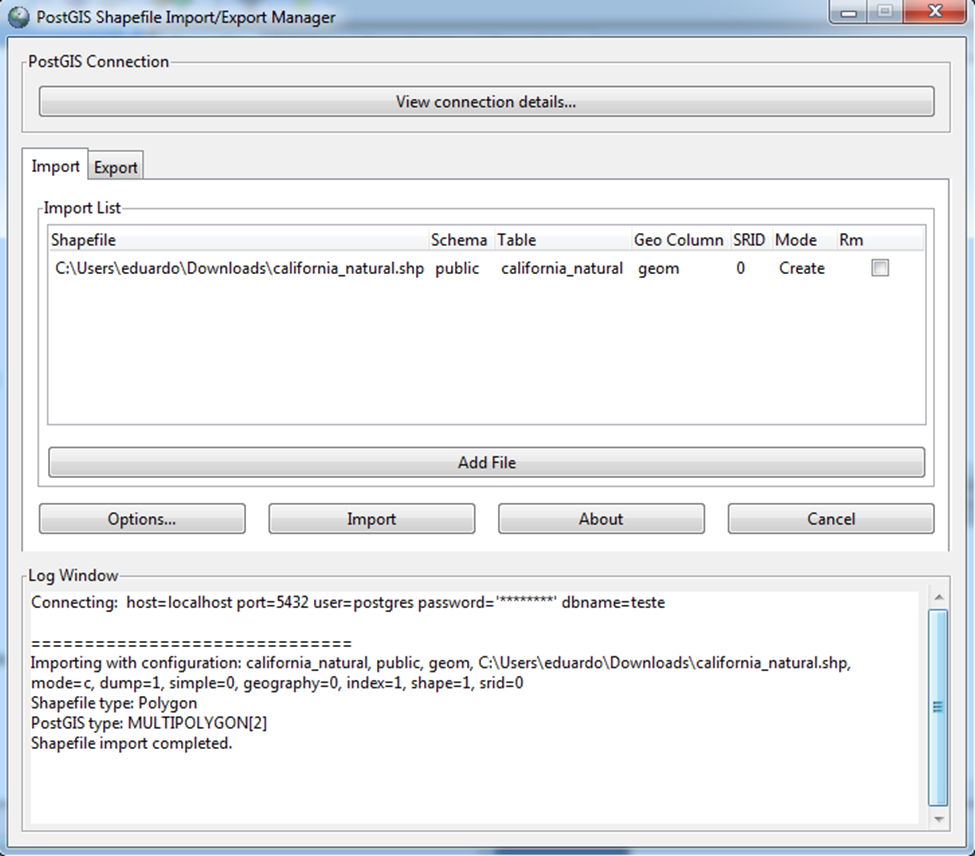
\includegraphics[width=1\linewidth]{data/shapefile_loader_gui}
		\caption{Interface gráfica do Shapefile and DBF Loader 2.1.}
		\label{fig:shapefileloadergui}
	\end{figure}
	
	\begin{figure}
		\centering
		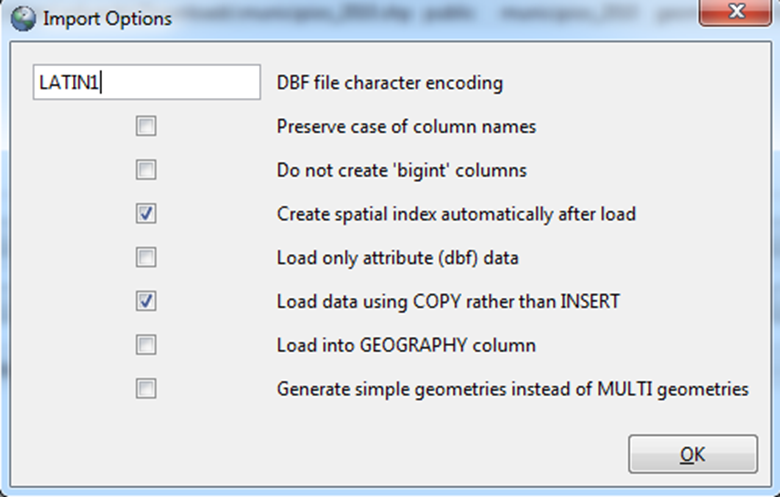
\includegraphics[width=1\linewidth]{data/import_config}
		\caption{Janela de configuração de importação. É interessante configurar o \textit{encoding} para LATIN1 para evitar caracteres estranhos e indesejados nos resultados das consultas.}
		\label{fig:importconfig}
	\end{figure}

	\section{Integração dos dados para análise}
	
	Com os dados já importados no PostGIS, é possível integrá-los com uma grande gama de aplicações tanto de forma offline quanto online. A partir daí muitas soluções de integração podem ser desenvolvidas. Uma bastante popular é representada na Figura \ref{fig:estruturaopensource} e utiliza a base de dados no PostGIS integrada ao Geoserver para a geração dos mapas consultados no PostGIS e visualizados em uma interface web como o OpenLayers. Uma abordagem mais específica e que demonstra todas as ferramentas e linguagens envolvidas no processo pode ser visto da Figura \ref{fig:estruturaopensource}. Outras já passam a utilizar tecnologias como Node.js com Express e Mapnik para criar servidores de mapas que processam a informação geográfica em "tempo real", sendo assim uma ótima alternativa para soluções em engenharia de tráfego e solucionamento de rotas, por exemplo.
	
	\begin{figure}
		\centering
		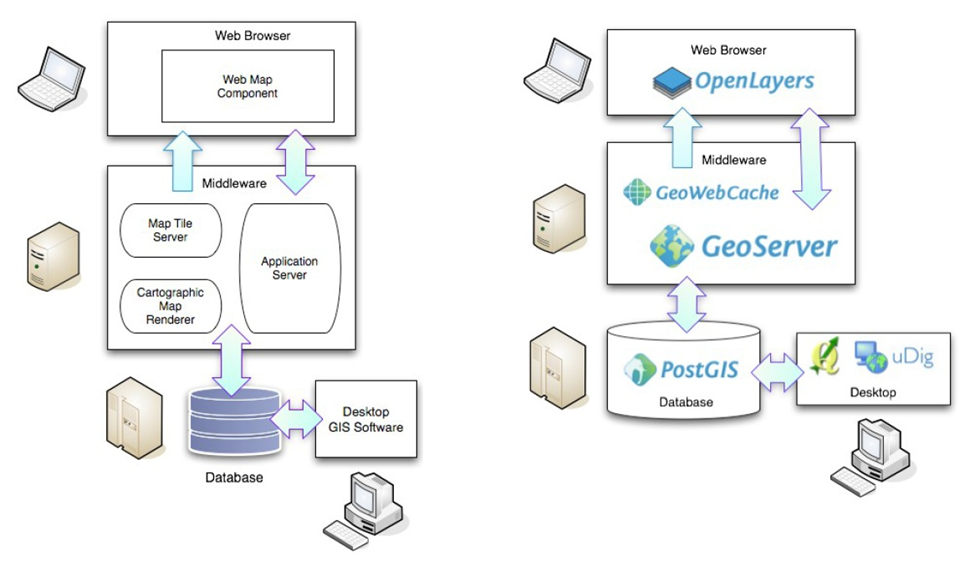
\includegraphics[width=1\linewidth]{data/estrutura_opensource}
		\caption{: Estrutura de código aberto que foi utilizada no trabalho e a representação da interface usuário/servidor. Autor: Carlos Cesar Gomes São Braz - IME(RJ)}
		\label{fig:estruturaopensource}
	\end{figure}

\newpage
	
No entanto, uma das principais e mais antigas ferramentas que possibilitam esta integração com o PostGIS é o QuantumGIS ou QGIS (Figura \ref{fig:diagrama}). O QGIS foi concebido inicialmente como uma ferramenta de conexão a bancos de dados PostgreSQL que utilizassem a extensão espacial PostGIS, mas que ao mesmo tempo tivesse como diferencial a funcionalidade de permitir a visualização do conteúdo geográfico para além das tabelas. O software amadureceu e hoje tem como bandeira ser o maior SIG gratuito e de código livre no mundo. No entanto, seu lado voltado aos bancos de dados desenvolveu somente até certo ponto. Em sua última versão estável 2.14 e mesmo em sua recém lançada versão de testes 2.16, o QGIS possui como padrão apenas a função de conexão e integração dos dados do PostGIS com o SIG. Alguns \textit{plugins} foram sendo desenvolvidos com o tempo por usuários que tentavam criar alternativas que buscassem simplificar ainda mais a utilização das funções exclusivas que o PostGIS possui. No entanto, nenhuma das alternativas apresentou, até o momento, uma interface que garanta um nível de abstração suficiente para que um usuário final que não saiba realizar consultas em SQL passe a utilizar estas funções espaciais.	

	\begin{figure}
		\centering
		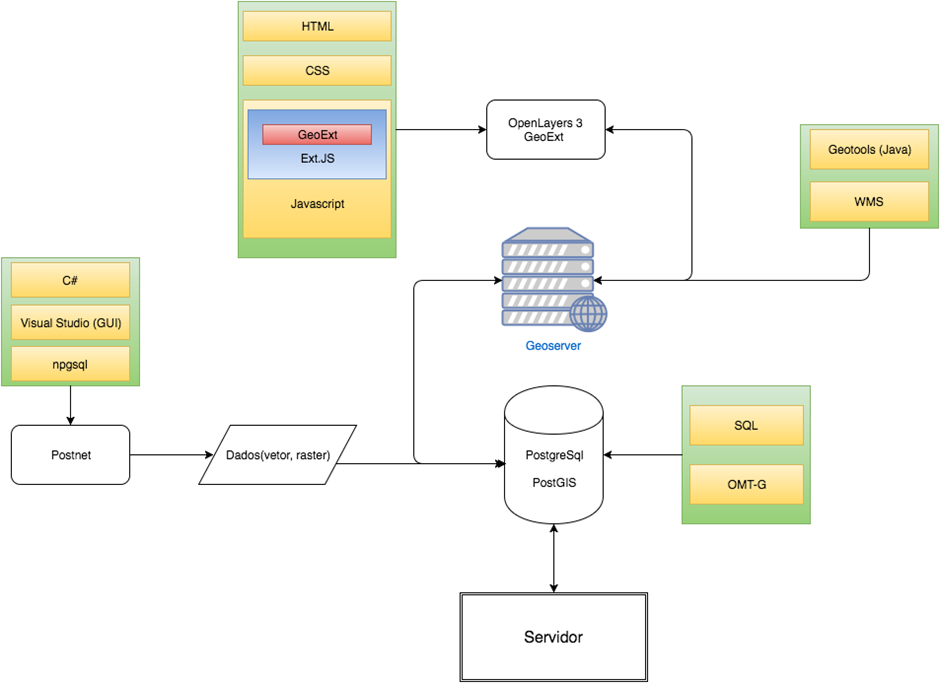
\includegraphics[width=1\linewidth]{data/diagrama}
		\caption{Diagrama com as ferramentas de análise, linguagens, recursos, suas conexões, camadas de abstração e tecnologias envolvidas.}
		\label{fig:diagrama}
	\end{figure}
	

	\begin{figure}
		\centering
		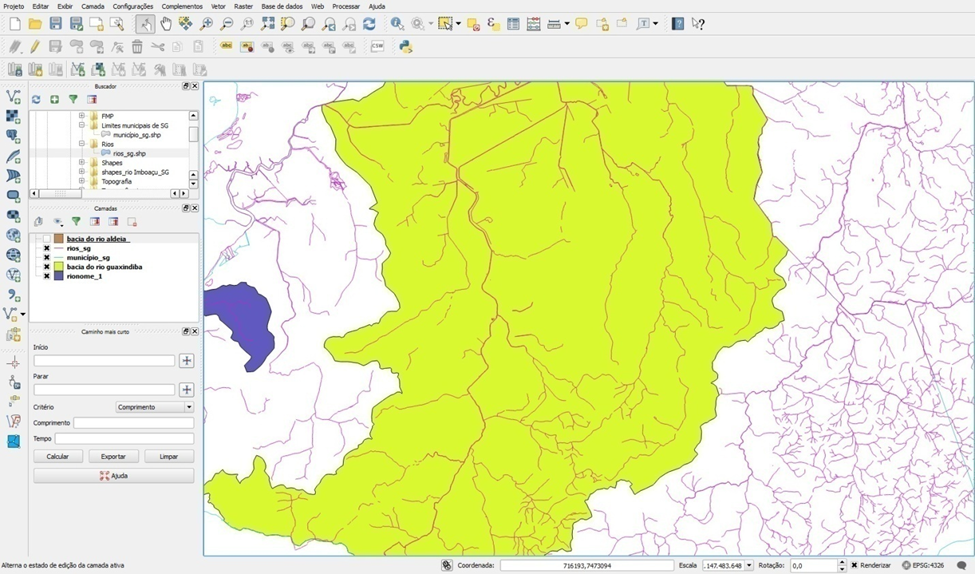
\includegraphics[width=1\linewidth]{data/qgis_gui}
		\caption{Interface gráfica do SIG QuantumGIS Desktop.}
		\label{fig:qgisgui}
	\end{figure}

A partir da proposta deste trabalho, pudemos notar nos capítulos anteriores que a utilização, por geógrafos, de banco de dados sejam eles geográficos ou não, na verdade já ocorre com certa frequência, mesmo que possibilitada por uma camada de abstração normalmente representada por uma funcionalidade do SIG como no caso do Geodatabase da ESRI. No entanto, por não existir um tipo de interface como o Geodatabase para plataformas livres, é importante considerar alternativas para que geógrafos e geocientistas de forma geral que utilizam ferramentas geoinformacionais livres também possam se beneficiar do uso de um SGBDOR, além de funcionalidades exclusivas sem que seja necessário aprender noções de programação e/ou SQL. 

Sendo assim, este trabalho buscou solucionar parte desse problema ao criar um software protótipo que possua uma interface gráfica que possibilite o usuário sem conhecimento técnico específico em programação, manipular informações geográficas mesmo que em grandes quantidades com o maior desempenho possível utilizando as funções de análise espacial do PostGIS.

Todo o desenvolvimento do software foi realizado utilizando a linguagem de programação C\# (C Sharp) através do \textit{framework} .NET e da IDE (\textit{Integrated Development Environment} -  Ambiente de Desenvolvimento Integrado) Microsoft Visual Studio 2015. C\# é uma linguagem interpretada multi-paradigma, fortemente tipada, e possui paradigmas de programação imperativa, funcional declarativa, genérica e principalmente orientada à objetos. É uma linguagem que foi desenvolvida pela Microsoft e foi apresentada oficialmente ao público em 2001 como parte do \textit{framework} .NET. por uma equipe montada e liderada por Anders Hejlsberg, criador do Delphi e do Turbo Pascal. Assim como Java, necessita ser compilada para \textit{bytecode} e interpretada por uma máquina virtual, neste caso, a \textit{Common Language Runtime} ou CLR. É uma linguagem que possui características muito próximas ao Java, o que por consequência faz com que grande parte das soluções desenvolvidas por ambas possuam características estruturais parecidas e possuam o mesmo "público alvo". A sintaxe utilizada pelo C\# se assemelha a vista em linguagens como C e C++, mesmo não possuindo relação direta com as mesmas. Além disso, linguagens como C e C++ possuem um processo de desenvolvimento muito mais complexo e são compiladas diretamente e especificamente para a arquitetura no qual o código foi compilado. 

Outra proposta do C\# (assim como do Java), é o de gerar códigos mais seguros e com menos chance de erros relacionados ao uso da memória. Em linguagens como C/C++, a utilização de ponteiros e a possibilidade de manipulação da memória ram através da \textit{Stack} e da \textit{Heap}, são essenciais para o desenvolvimento de softwares que buscam alto desempenho, mas necessitam que o programador saiba exatamente como e onde cada segmento de memória está sendo alocado e desalocado. Caso contrário, o programa tende a apresentar um número muito maior de \textit{bugs} e um uso excessivo de memória. Além disso, em projetos maiores e com número maior de linhas de código, a manutenção tende a ser muito mais complexa, assim como a identificação de erros relacionado ao mau uso de recursos. Tanto o C\# quanto o Java, são linguagens em que a utilização de recursos é em grande parte trabalho da máquina virtual e é consequentemente realizada de forma automática, sem que o desenvolvedor tenha que se preocupar. No entanto, há perda de desempenho.

Java foi por muito tempo a linguagem para aplicações \textit{desktop} que possuía um lado web que dominou a área do desenvolvimento geotecnológico. Ferramentas como o GeoTools, GeoServer, JTS Topology Suite, Gisgraphy, e o World Wind Java SDK desenvolvido pela NASA, são bons exemplos de como a comunidade de desenvolvedores SIG tinham uma preferência clara em relação à linguagem Java. O provável motivo para tal preferência eram as características multi-plataforma de uma linguagem livre como o Java e seu consequente crescimento em todo o mercado de TI. O C\#, por ter sido desenvolvido pela Microsoft tinha como limitação a dependência do sistema Windows para rodar suas aplicações. No entanto, com o tempo, muitas soluções multi-plataformas foram surgindo como o Mono e posteriormente o Xamarin até a liberação total das bibliotecas padrões oficialmente pela Microsoft. Sendo assim, hoje em dia, C\# é uma linguagem de programação livre e também multi-plataforma (Windows, Linux, OSX, Android, iOS, Windows Phone, etc). 

Na área geoespacial, algumas ferramentas importantes foram desenvolvidas nos últimos 15 anos utilizando C\# como o SharpMap.NET, o NTS Topology Suite (versão em C\# do JTS escrito em Java), o GeoLib, o Nutiteq Maps SDK (para plataformas mobile), e mais recentemente o DotSpatial, ferramenta base deste trabalho.

O DotSpatial é uma biblioteca escrita originalmente para o \textit{framework} .NET 4 utilizando a linguagem C\# como uma solução para incorporar funções SIG para outras aplicações. Este projeto utilizou o DotSpatial para adicionar funções básicas de manipulação de dados georreferenciados em um ambiente simples. Além disso, o sistema possui uma segunda interface para a manipulação de funções espaciais do PostGIS. 

Toda a funcionalidade de conexão com o banco de dados PostgreSQL/PostGIS foi realizada utilizando-se da biblioteca Npgsql (NPGSQL, 2016) buscando utilizar as funcionalidades proporcionadas pelo paradigma da programação orientada a objetos.

Sendo assim, através da possibilidade de utilização das citadas ferramentas iniciou-se o processo de desenvolvimento de um Sistema de Informações Geográficas protótipo denominado espaçoGIS (Figura \ref{fig:espacogislogo}).

	\begin{figure}
		\centering
		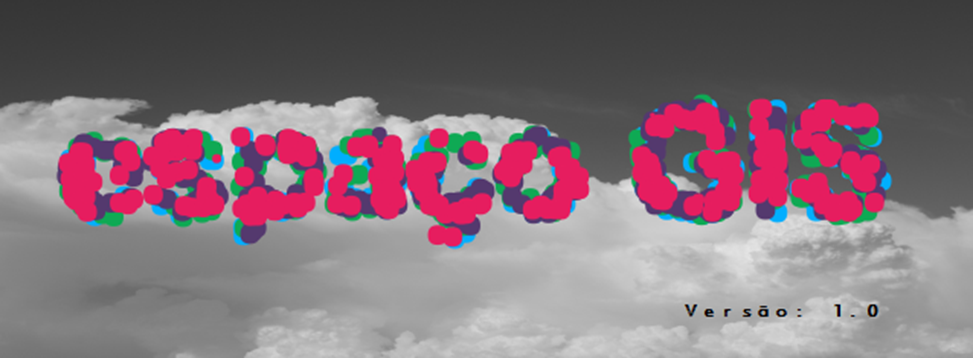
\includegraphics[width=1\linewidth]{data/espacoGIS_logo}
		\caption{Logo do Sistema de Informação Geográfico espaçoGIS.}
		\label{fig:espacogislogo}
	\end{figure}

O protótipo utiliza uma interface de documentos múltiplos (MDI - \textit{Multiple Document Interface}) para gerenciar as janelas, dando a possibilidade de gerenciamento dos diversos módulos pertencentes ao SIG espaçoGIS (Figura \ref{fig:espacogisgui}), como o módulo SIG e o módulo de funcionalidades e gerenciamento de bancos de dados no PostGIS denominado PostNet (Figura \ref{fig:postnetgui}). Na Figura \ref{fig:mdigui} apresenta a vantagem do uso de uma interface do tipo MDI.

	\begin{figure}
		\centering
		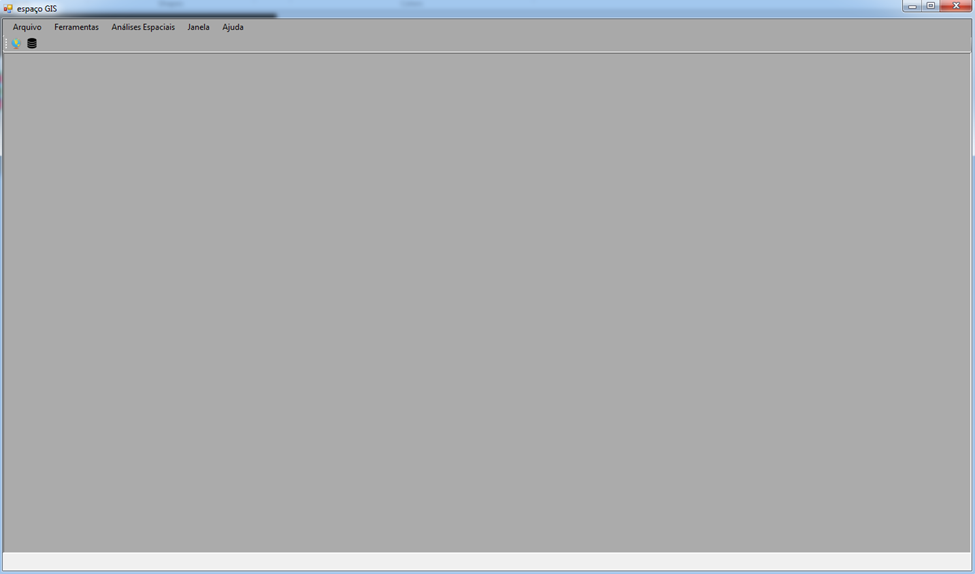
\includegraphics[width=0.8\linewidth]{data/espacoGIS_gui}
		\caption{Apresentação inicial da interface do sistema espaçoGIS.}
		\label{fig:espacogisgui}
	\end{figure}
	
	\begin{figure}
		\centering
		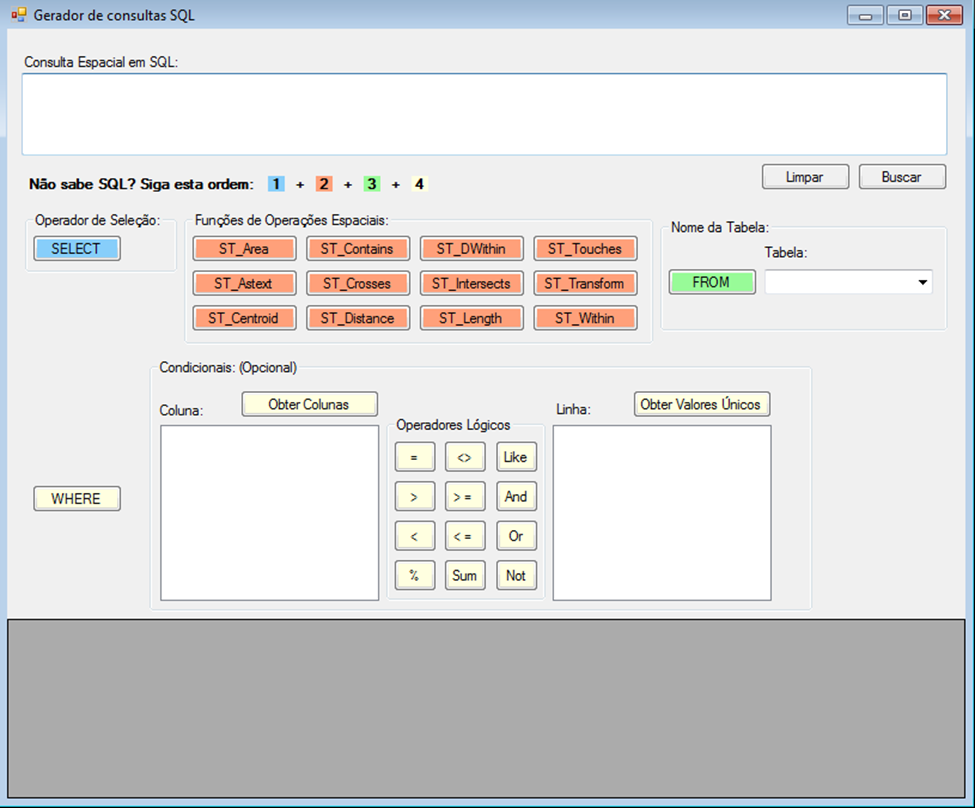
\includegraphics[width=1\linewidth]{data/postnet_gui}
		\caption{Módulo PostNET ou "Gerenciador de Consultas SQL".}
		\label{fig:postnetgui}
	\end{figure}

	\begin{figure}
		\centering
		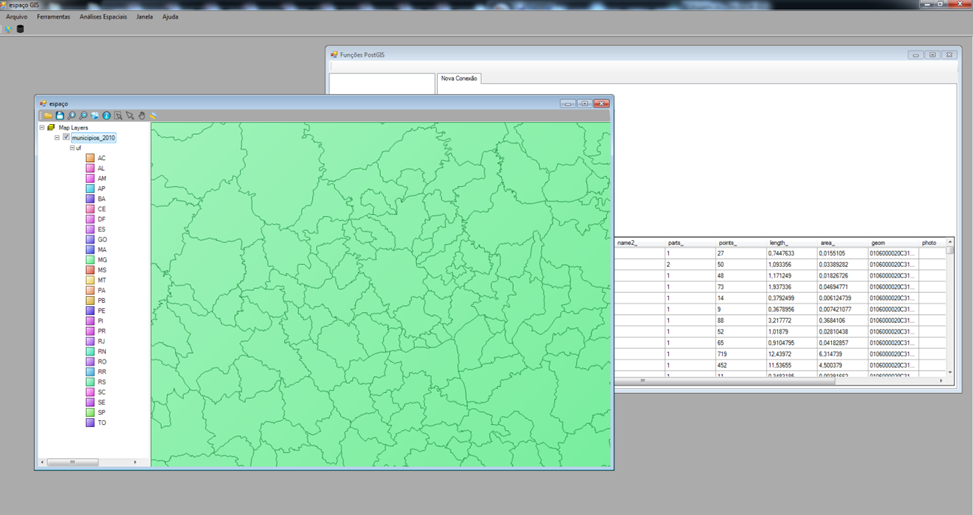
\includegraphics[width=1\linewidth]{data/mdi_gui}
		\caption{A escolha pelo uso de um MDI se deu em função da implementação de diversos módulos em um mesmo sistema.}
		\label{fig:mdigui}
	\end{figure}

A implementação do módulo SIG se deu primeiramente desenvolvendo as funcionalidades mais básicas utilizando a biblioteca DotSpatial. Funções como "Adicionar Camada", "Zoom In", "Zoom Out", "Zoom to Extent", "Limpar Camada", "Informações", "Selecionar", "Pan" e "Salvar Camada" foram implementadas primeiramente como mostrado no Anexo.

Em seguida, o módulo de funções ligadas à aba de legenda foi desenvolvida assim como o módulo de visualização dos mapas, representados respectivamente na Figura \ref{fig:siggui}.

A interface ainda possui a janela de conexão ao PostGIS (Figura \ref{fig:postgisconfig}) e ao módulo PostNET. A GUI (\textit{Guafical User Interface}) desenvolvida para as funções do módulo PostNet possuem um padrão específico, buscando se assemelhar propositalmente à interface do módulo "Selecionar por Atributos" desenvolvida para o SIG ArcMap. Esta escolha se deu devido a grande popularidade do software e por considerar que grande parte da comunidade envolvida com a utilização de SIG provavelmente já teve algum contato com a ferramenta da ESRI, facilitando o acesso de novos usuários.

	\begin{figure}
		\centering
		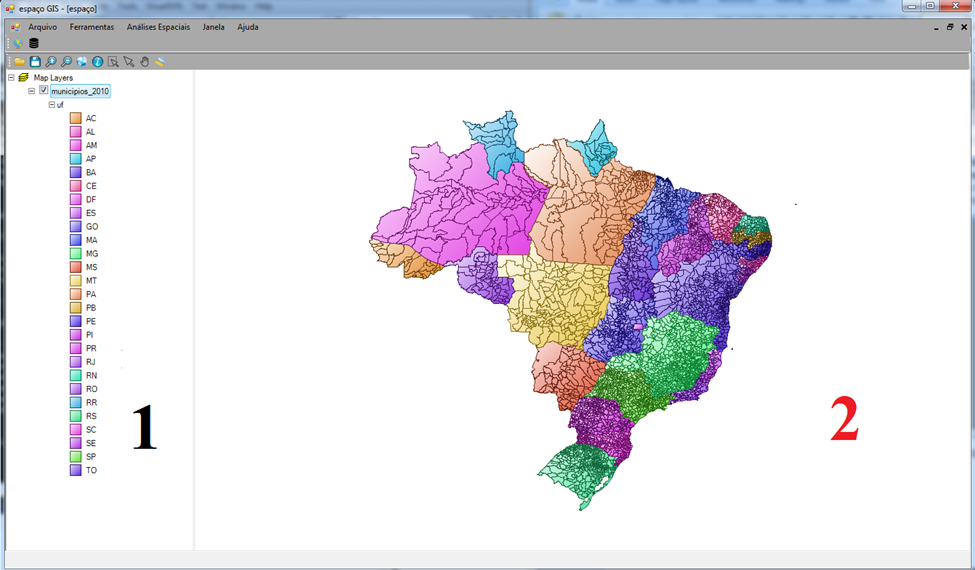
\includegraphics[width=1\linewidth]{data/sig_gui}
		\caption{A interface gráfica do módulo SIG é dividido basicamente entre duas áreas de visualização. A área de legenda, organização dos \textit{layers} e funcionalidades de visualização e exportação representada pelo número 1 e a área de visualização de mapas representada pelo número 2.}
		\label{fig:siggui}
	\end{figure}
	
	\begin{figure}
		\centering
		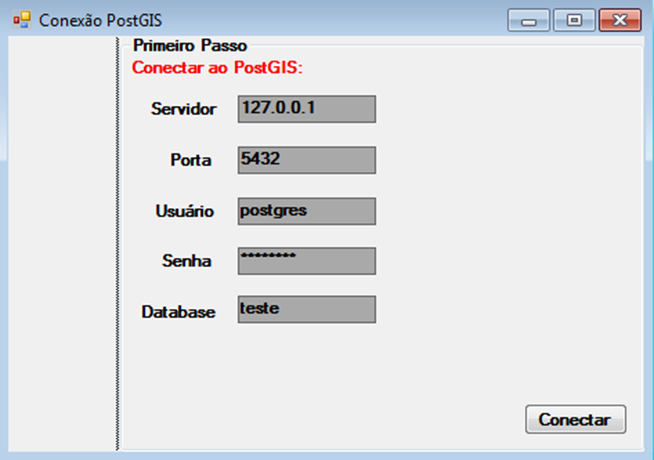
\includegraphics[width=0.7\linewidth]{data/postgis_config}
		\caption{Janela de configuração de conexão com o banco PostGIS.}
		\label{fig:postgisconfig}
	\end{figure}
	
O propósito pela criação de uma ferramenta com uma interface como o PostNET é a de facilitar o aprendizado da linguagem SQL padrão, assim como principalmente da sintaxe utilizada pelo módulo PostGIS.

\chapter{Considerações Finais}
A busca por uma Geografia mais conjuntiva, integrada e transdisciplinar é o que motiva a busca por novas metodologias de análise e futuras discussões epistemológicas de acordo com o constante avanço tecnológico. A percepção e inclusão da noção de espaço pela ciência atual como um aditivo ao conceito de tempo, já tradicional em muitos estudos, explica a necessidade por trabalhos que provoquem esta maior integração na Geografia. A preocupação pela inclusão da espacialidade ao explicar processos com mudanças ao longo do tempo gerou como resposta uma busca pelo desenvolvimento de ferramentas que suportem, de fato, estas análises. 

Além disso, o rápido desenvolvimento de tecnologias de armazenamento e processamento de dados digitais, assim como sua popularização e distribuição em massa geraram como consequência um aumento significativo na acumulação de informações espacializadas. No entanto, apesar de tal desenvolvimento, a Geografia parece, de forma geral, enfrentar limitações quando o assunto é a integração de métodos computacionais modernos ao processo de análise espacial. Limitações como esta tem origem epistemológica e são consequência de uma lógica do fazer científico que esbarra em uma histórica lógica Kuhniana de quebra de paradigmas. Entendendo o desenvolvimento do pensamento não só geográfico, como científico, principalmente durante o último século, nos revela que a busca por uma Geografia menos dicotômica pode ser a chave para uma ciência geográfica mais integrada e transdisciplinar.

A aplicação de métodos computacionais na Geografia possui uma longa história, e pelo o que o desenvolvimento de tecnologias recentes vem mostrando, esta relação tende a aumentar como nunca. Cabe, portanto a Geografia buscar entender como a aplicação de novas tecnologias pode sim influenciar na integração de análises geográficas quantitativas e qualitativas. 

Este trabalho buscou contribuir para a discussão mostrando que esta relação não necessariamente precisa ser feita através de grandes especialistas técnicos. Além disso, teve como objetivo a criação de uma ferramenta que possa servir como base para que pesquisadores ou qualquer maior interessado aprenda e utilize todo o potencial que os bancos de dados geográficos e suas análises espaciais disponibilizam.

O fazer científico atual baseado na acumulação de grandes bases de dados espaciais possui muitos perigos em sua utilização, principalmente quando tratado como finalidade. A Geografia, especialmente a brasileira, possui discussões conceituais aprofundadas que podem ajudar este novo paradigma a encontrar um caminho um pouco mais crítico. No entanto, é necessário que se olhe para novas tecnologias sem o medo burro do preconceito e entendendo que o fazer científico, sendo quantitativo ou não, deve ser feito com consciência. 

Além disso, compreender as funcionalidades existentes nas implementações dos SIG existentes nos dá a possibilidade de entender o processo de produção do conhecimento geotecnológico compatível com as limitações impostas pela tecnologia desenvolvida. Ou seja, se o software de SIG padrão determina a pesquisa e a prática do SIG, a utilização de bancos de dados geográficos que permitam uma análise geográfica mais completa e funcional, podem por consequência influenciar na produção de estudos geográficos mais complexos.

A criação de novas técnicas e ferramentas é constante e foi percebida na própria realização deste trabalho devido as constantes atualizações na bibliografia. Buscou-se citar a maior parte das principais ferramentas de análise espacial ligadas a utilização de bancos de dados geográficos, no entanto, não há tempo para um estudo mais aprofundado para cada tecnologia. Priorizou-se então a busca em entender a diversidade de ferramentas e métodos.

De forma geral, a Geografia brasileira atual buscar formar o novo geógrafo centrado no entendimento de seus conceitos fundamentais e na realização de análises geográficas de forma a considerar particularidades, ações e objetos em múltiplas escalas. A aplicação de conceitos como o de holística e complexidade surgem neste contexto como uma sensação de otimismo aos que não conseguem entender duas geografias. De acordo com o aprimoramento tecnológico, pouco a pouco, conceitos fundamentais da Geografia talvez poderão ser aplicados a novas soluções. Cabe a Geografia então servir como norteadora para um desenvolvimento geotecnológico, de fato, mais integrado.
	
	\bibliographystyle{plain}
	\bibliography{referencias}
	
	\appendix
	\chapter{Estrutura do código fonte do Gerador de Consultas SQL para PostGIS (PostNET)}

A ferramenta de geração de consultas em SQL para PostGIS serve como uma interface gráfica para estimular o aprendizado e a utilização da ferramenta PostGIS assim como uma ferramenta para o ensino da linguagem SQL. Além disso, o módulo se propõe a servir como uma plataforma de ensino da manipulação e análise de dados espaciais utilizando banco de dados geográficos. O software foi desenvolvido no Microsoft Visual Studio 2015 utilizando a linguagem de programação C\#. O código a seguir é referente ao módulo PostGIS que pode ser visualizado na Figura \ref{fig:postnetguiquery}:

	\begin{figure}
		\centering
		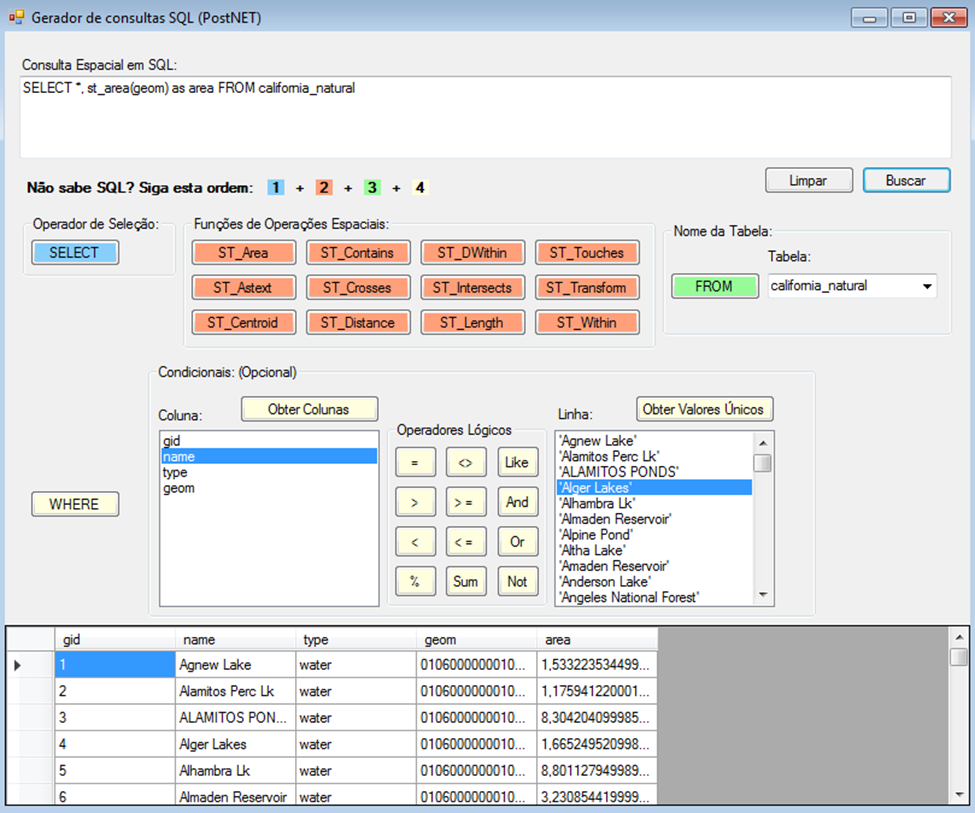
\includegraphics[width=1\linewidth]{data/postnet_gui_query}
		\caption{Interface gráfica do Gerador de Consultas SQL (PostGIS)}
		\label{fig:postnetguiquery}
	\end{figure}

\newpage
	
\begin{lstlisting}
	using System;
	using System.Collections.Generic;
	using System.ComponentModel;
	using System.Data;
	using System.Drawing;
	using System.Linq;
	using System.Text;
	using System.Windows.Forms;
	using Npgsql;
	
	namespace espacoGIS
	{
	public partial class sqlQuery : Form
	{
	public string sql;
	
	// mFrom = false => uma tabela (1x geom)
	// mFrom = true => duas tabelas (2x geom)
	bool mFrom = false;
	
	public sqlQuery()
	{
	InitializeComponent();
	getTables();
	}
	
	/// <summary>
	/// Conecta ao banco PostGIS e realiza a consulta de acordo com o texto no TextBox.
	/// </summary>
	/// <param name="sender"></param>
	/// <param name="e"></param>
	private void buscar_btn_Click(object sender, EventArgs e)
	{
	connQuery();
	}
	
	private void connQuery()
	{
	if (sqlQuery_txt.Text == "")
	{
	MessageBox.Show("Digite o comando primeiro!");
	}
	try
	{
	ConexaoDB postgis = new ConexaoDB();
	NpgsqlConnection conn = new NpgsqlConnection(postgis.connOpenDB());
	NpgsqlDataAdapter dbda = new NpgsqlDataAdapter(sqlQuery_txt.Text, conn);
	DataTable dbdataset = new DataTable();
	dbda.Fill(dbdataset);
	dataGridView1.DataSource = dbdataset;
	
	//Da um Bind Data Source e mostra os dados no dataGridView.
	BindingSource bsource = new BindingSource();
	bsource.DataSource = dbdataset;
	dataGridView1.DataSource = bsource;
	conn.Close();
	}
	catch (Exception ex)
	{
	MessageBox.Show(ex.Message);
	}
	}
	
	private void getTables()
	{
	string sql_tables = "SELECT table_name FROM information_schema.tables WHERE table_schema = 'public';";
	
	// Logica de conexao
	ConexaoDB postgis = new ConexaoDB();
	NpgsqlConnection conn = new NpgsqlConnection(postgis.connOpenDB());
	NpgsqlCommand cm = new NpgsqlCommand(sql_tables, conn);
	NpgsqlDataReader reader;
	try
	{
	conn.Open();
	reader = cm.ExecuteReader();
	while (reader.Read())
	{
	string stables = reader.GetString(0);
	tables_cbx.Items.Add(stables);
	}
	conn.Close();
	}
	catch (Exception ex)
	{
	MessageBox.Show(ex.Message);
	}
	}
	
	public void getColumns()
	{
	if (tables_cbx.Text != "")
	{
	// Limpa a ListBox antes de fazer uma nova pesquisa
	coluna_listbox.Items.Clear();
	
	string tabela = tables_cbx.Text;
	string sql_columns = "SELECT column_name FROM information_schema.columns WHERE table_schema = 'public' AND table_name = '" + tables_cbx.Text + "'";
	
	// Logica de conexao
	ConexaoDB postgis = new ConexaoDB();
	NpgsqlConnection conn = new NpgsqlConnection(postgis.connOpenDB());
	NpgsqlCommand cm = new NpgsqlCommand(sql_columns, conn);
	NpgsqlDataReader reader;
	try
	{
	conn.Open();
	reader = cm.ExecuteReader();
	while (reader.Read())
	{
	string colunas = reader.GetString(0);
	coluna_listbox.Items.Add(colunas);
	}
	conn.Close();
	}
	catch (Exception ex)
	{
	MessageBox.Show(ex.Message);
	}
	}
	}
	
	private void getRows()
	{
	if (coluna_listbox.Text != "")
	{
	// Limpa a ListBox antes de fazer uma nova pesquisa
	rows_listbox.Items.Clear();
	
	string tabela = tables_cbx.Text;
	string linha = coluna_listbox.GetItemText(coluna_listbox.SelectedItem);
	string sql_rows = "SELECT " + linha + " FROM " + tabela;
	
	// Logica de conexao
	ConexaoDB postgis = new ConexaoDB();
	NpgsqlConnection conn = new NpgsqlConnection(postgis.connOpenDB());
	NpgsqlCommand cm = new NpgsqlCommand(sql_rows, conn);
	NpgsqlDataReader reader;
	try
	{
	conn.Open();
	reader = cm.ExecuteReader();
	while (reader.Read())
	{
	string rows = reader.GetString(0);
	string xrows = "'" + rows + "'";
	rows_listbox.Items.Add(xrows);
	}
	conn.Close();
	}
	catch (Exception ex)
	{
	MessageBox.Show(ex.Message);
	}
	}
	}
	
	#region botoes query sql
	/// <summary>
	/// Adiciona o operador SELECT ao texto da query SQL.
	/// O valor * e dado como padrao.
	/// </summary>
	/// <param name="sender"></param>
	/// <param name="e"></param>
	private void select_btn_Click(object sender, EventArgs e)
	{
	sql += "SELECT *, ";
	sqlQuery_txt.Text = sql;
	}
	
	/// <summary>
	/// Adiciona o operador FROM ao texto da query SQL.
	/// Checa se o valor mFrom e true ou false.
	/// O valor false funciona para realizar funcoes que 
	/// necessitam de apenas uma geometria ("geom").
	/// Se o mFrom for true, o botao FROM adiciona o texto 
	/// especifico para duas geometrias.
	/// </summary>
	/// <param name="sender"></param>
	/// <param name="e"></param>
	private void from_btn_Click(object sender, EventArgs e)
	{
	if (mFrom == false && tables_cbx.Text == "")
	{
	sql += "FROM nome_da_tabela ";
	sqlQuery_txt.Text = sql;
	}
	else if (mFrom == false)
	{
	sql += "FROM " + tables_cbx.Text + " ";
	sqlQuery_txt.Text = sql;
	}
	else
	{
	sql += "FROM nome_da_tabela g1, nome_da_outra_tabela g2 ";
	sqlQuery_txt.Text = sql;
	}
	}
	
	/// <summary>
	/// Adiciona o operador WHERE ao texto da query SQL.
	/// </summary>
	/// <param name="sender"></param>
	/// <param name="e"></param>
	private void where_btn_Click(object sender, EventArgs e)
	{
	if (coluna_listbox.Items.Count > 0)
	{
	sql += "WHERE " + coluna_listbox.Text + " ";
	sqlQuery_txt.Text = sql;
	}
	else
	{
	sql += "WHERE ";
	sqlQuery_txt.Text = sql;
	}
	}
	
	/// <summary>
	/// Adiciona a funcao ST_Area ao texto da query SQL.
	/// </summary>
	/// <param name="sender"></param>
	/// <param name="e"></param>
	public void stArea_btn_Click(object sender, EventArgs e)
	{
	sql += "st_area(geom) as area ";
	sqlQuery_txt.Text = sql;
	}
	
	/// <summary>
	/// Adiciona a funcao ST_Length ao texto da query SQL.
	/// </summary>
	/// <param name="sender"></param>
	/// <param name="e"></param>
	private void stLength_btn_Click(object sender, EventArgs e)
	{
	sql += "st_length(geom) ";
	sqlQuery_txt.Text = sql;
	}
	
	/// <summary>
	/// Limpa o campo de busca.
	/// Troca o valor de mFrom para seu valor default: false.
	/// </summary>
	/// <param name="sender"></param>
	/// <param name="e"></param>
	private void limpar_btn_Click(object sender, EventArgs e)
	{
	sql = "";
	sqlQuery_txt.Text = sql;
	mFrom = false;
	}
	
	/// <summary>
	/// Adiciona a funcao ST_Within ao texto da query SQL.
	/// Troca o valor de mFrom para "true".
	/// </summary>
	/// <param name="sender"></param>
	/// <param name="e"></param>
	private void stWithin_btn_Click(object sender, EventArgs e)
	{
	sql += "st_within(g1.geom, g2.geom) ";
	sqlQuery_txt.Text = sql;
	mFrom = true;
	}
	
	/// <summary>
	/// Adiciona o operador de comparacao "=" (igual) ao texto da query SQL.
	/// </summary>
	/// <param name="sender"></param>
	/// <param name="e"></param>
	private void iqual_btn_Click(object sender, EventArgs e)
	{
	sql += " = ";
	sqlQuery_txt.Text = sql;
	}
	
	/// <summary>
	/// Adiciona o operador de comparacao "<>" (not iqual) ao texto da query SQL.
	/// </summary>
	/// <param name="sender"></param>
	/// <param name="e"></param>
	private void notIqual_btn_Click(object sender, EventArgs e)
	{
	sql += " <> ";
	sqlQuery_txt.Text = sql;
	}
	
	/// <summary>
	/// Adiciona o operador de comparacao ">" (maior que) ao texto da query SQL.
	/// </summary>
	/// <param name="sender"></param>
	/// <param name="e"></param>
	private void maiorQ_btn_Click(object sender, EventArgs e)
	{
	sql += " > ";
	sqlQuery_txt.Text = sql;
	}
	
	/// <summary>
	/// Adiciona o operador de comparacao "<" (menor que) ao texto da query SQL.
	/// </summary>
	/// <param name="sender"></param>
	/// <param name="e"></param>
	private void menorQ_btn_Click(object sender, EventArgs e)
	{
	sql += " < ";
	sqlQuery_txt.Text = sql;
	}
	
	/// <summary>
	/// Adiciona o operador de comparacao ">=" (maior ou igual) ao texto da query SQL.
	/// </summary>
	/// <param name="sender"></param>
	/// <param name="e"></param>
	private void maiorOuIqual_btn_Click(object sender, EventArgs e)
	{
	sql += " >= ";
	sqlQuery_txt.Text = sql;
	}
	
	/// <summary>
	/// Adiciona o operador de comparacao "<=" (menor ou igual) ao texto da query SQL.
	/// </summary>
	/// <param name="sender"></param>
	/// <param name="e"></param>
	private void menorOuIqual_btn_Click(object sender, EventArgs e)
	{
	sql += " <= ";
	sqlQuery_txt.Text = sql;
	}
	
	/// <summary>
	/// Adiciona o operador logico "ILIKE" ao texto da query SQL.
	/// </summary>
	/// <param name="sender"></param>
	/// <param name="e"></param>
	private void like_btn_Click(object sender, EventArgs e)
	{
	sql += " ILIKE ";
	sqlQuery_txt.Text = sql;
	}
	
	/// <summary>
	/// Adiciona o operador logico "AND" ao texto da query SQL.
	/// </summary>
	/// <param name="sender"></param>
	/// <param name="e"></param>
	private void and_btn_Click(object sender, EventArgs e)
	{
	sql += " AND ";
	sqlQuery_txt.Text = sql;
	}
	
	/// <summary>
	/// Adiciona o operador logico "OR" ao texto da query SQL.
	/// </summary>
	/// <param name="sender"></param>
	/// <param name="e"></param>
	private void or_btn_Click(object sender, EventArgs e)
	{
	sql += " OR ";
	sqlQuery_txt.Text = sql;
	}
	
	/// <summary>
	/// Adiciona o operador logico "NOT" ao texto da query SQL.
	/// </summary>
	/// <param name="sender"></param>
	/// <param name="e"></param>
	private void not_btn_Click(object sender, EventArgs e)
	{
	sql += " NOT ";
	sqlQuery_txt.Text = sql;
	}
	
	/// <summary>
	/// Adiciona a funcao "sum" (soma) ao texto da query SQL.
	/// </summary>
	/// <param name="sender"></param>
	/// <param name="e"></param>
	private void sum_btn_Click(object sender, EventArgs e)
	{
	sql += "sum( ";
	sqlQuery_txt.Text = sql;
	}
	
	/// <summary>
	/// Adiciona o sibolo "%" ao texto da query SQL.
	/// Serve para realizar buscas atraves de palavras especificas.
	/// </summary>
	/// <param name="sender"></param>
	/// <param name="e"></param>
	private void porcentagem_btn_Click(object sender, EventArgs e)
	{
	sql += "%";
	sqlQuery_txt.Text = sql;
	}
	
	/// <summary>
	/// Adiciona a funcao ST_Touches ao texto da query SQL.
	/// </summary>
	/// <param name="sender"></param>
	/// <param name="e"></param>
	private void stTouches_btn_Click(object sender, EventArgs e)
	{
	sql += "st_touches(g1.geom, g2.geom) ";
	sqlQuery_txt.Text = sql;
	mFrom = true;
	}
	
	/// <summary>
	/// Adiciona a funcao ST_Transform ao texto da query SQL.
	/// E necessario adicionar o SRID correto.
	/// </summary>
	/// <param name="sender"></param>
	/// <param name="e"></param>
	private void stTransform_btn_Click(object sender, EventArgs e)
	{
	sql += "st_transform(geom, SRID) ";
	sqlQuery_txt.Text = sql;
	}
	
	/// <summary>
	/// Adiciona a funcao ST_DWithin ao texto da query SQL.
	/// </summary>
	/// <param name="sender"></param>
	/// <param name="e"></param>
	private void stDwithin_btn_Click(object sender, EventArgs e)
	{
	sql += "st_within(g1.geom, g2.geom, distancia_em_metros) ";
	sqlQuery_txt.Text = sql;
	mFrom = true;
	}
	
	/// <summary>
	/// Adiciona a funcao ST_Crosses ao texto da query SQL.
	/// </summary>
	/// <param name="sender"></param>
	/// <param name="e"></param>
	private void stCrosses_btn_Click(object sender, EventArgs e)
	{
	sql += "st_crosses(g1.geom, g2.geom) ";
	sqlQuery_txt.Text = sql;
	mFrom = true;
	}
	
	/// <summary>
	/// Adiciona a funcao ST_Centroid ao texto da query SQL.
	/// </summary>
	/// <param name="sender"></param>
	/// <param name="e"></param>
	private void stCentroid_btn_Click(object sender, EventArgs e)
	{
	sql += "st_centroid(geom) ";
	sqlQuery_txt.Text = sql;
	}
	
	/// <summary>
	/// Adiciona a funcao ST_AsText ao texto da query SQL.
	/// </summary>
	/// <param name="sender"></param>
	/// <param name="e"></param>
	private void stAsText_btn_Click(object sender, EventArgs e)
	{
	sql += "st_astext(geom) ";
	sqlQuery_txt.Text = sql;
	mFrom = false;
	}
	
	/// <summary>
	/// Adiciona a funcao ST_Contains ao texto da query SQL.
	/// </summary>
	/// <param name="sender"></param>
	/// <param name="e"></param>
	private void stContains_btn_Click(object sender, EventArgs e)
	{
	sql += "st_contains(g1.geom, g2.geom) ";
	sqlQuery_txt.Text = sql;
	mFrom = true;
	}
	
	/// <summary>
	/// Adiciona a funcao ST_Distance ao texto da query SQL.
	/// </summary>
	/// <param name="sender"></param>
	/// <param name="e"></param>
	private void stDistance_btn_Click(object sender, EventArgs e)
	{
	sql += "st_distance(g1.geom, g2.geom) ";
	sqlQuery_txt.Text = sql;
	}
	
	/// <summary>
	/// Adiciona a funcao ST_Intersects ao texto da query SQL.
	/// </summary>
	/// <param name="sender"></param>
	/// <param name="e"></param>
	private void stintersects_btn_Click(object sender, EventArgs e)
	{
	sql += "st_intersects(g1.geom, g2.geom) ";
	sqlQuery_txt.Text = sql;
	mFrom = true;
	}
	
	/// <summary>
	/// Carrega as colunas da tabela selecionada
	/// </summary>
	/// <param name="sender"></param>
	/// <param name="e"></param>
	private void getColunas_btn_Click(object sender, EventArgs e)
	{
	getColumns();
	}
	
	/// <summary>
	/// Carrega as linhas da tabela selecionada
	/// </summary>
	/// <param name="sender"></param>
	/// <param name="e"></param>
	private void getUniqueValues_btn_Click(object sender, EventArgs e)
	{
	getRows();
	}
	
	private void coluna_listbox_MouseDoubleClick(object sender, MouseEventArgs e)
	{
	sql += coluna_listbox.SelectedItem;
	sqlQuery_txt.Text = sql;
	}
	
	private void rows_listbox_MouseDoubleClick(object sender, MouseEventArgs e)
	{
	sql += rows_listbox.SelectedItem;
	sqlQuery_txt.Text = sql;
	}
	#endregion
	}
	}
\end{lstlisting}
	
\end{document}